\documentclass[10pt]{article}		% sets document class
\usepackage[usenames,dvipsnames]{pstricks}
\usepackage{epsfig}
\usepackage{pst-grad} 				% enables gradients
\usepackage{pst-plot} 				% enables axes
\usepackage[space]{grffile} 		% enables spaces in paths
\usepackage{etoolbox} 				% enables spaces in paths
\makeatletter 						% enables spaces in paths
\patchcmd\Gread@eps{\@inputcheck#1 }{\@inputcheck"#1"\relax}{}{}
\makeatother
\usepackage[margin=1.0in]{geometry}	% sets paper size
\usepackage{amssymb}				% enables formulas
\usepackage{amsmath}				% enables formulas
\usepackage[utf8]{inputenc}			% enables diacritical input
\usepackage{graphicx}				% enables graphics
\graphicspath{ {images/} }			% sets graphics path
\usepackage{chngcntr}				% enables counter
\counterwithin{table}{subsection}	% enables table pre-labels
\counterwithin{figure}{subsection}	% enables figure pre-labels
\usepackage[labelsep=endash, labelfont=bf, font=bf]{caption}	% sets figure and caption separator
%\usepackage{indentfirst}			% enables indent on first paragraphs
\linespread{1.1}					% sets spacing to 1.5
\setlength{\parskip}{0.5em}			% sets paragraph spacing to 1m
%\usepackage{times}					% sets font to times new roman
\usepackage{wrapfig}				% enables text wrapping around figures
\usepackage{gensymb}				% enables symbols
\usepackage{endnotes}				% enables endnotes
\usepackage{afterpage}				% enables afterpage capability
\setcounter{secnumdepth}{3}			% sets counter recognitions to sssection for label capability
\numberwithin{equation}{section}
\makeatletter						% set figure labels to center
\g@addto@macro\@floatboxreset\centering
\makeatother
\usepackage{setspace}				% enables environments for spacing
\usepackage{graphicx}				% allows table usage
\usepackage{hyperref}				% enables hyperlinks
\hypersetup{colorlinks=false, linkcolor=cyan, urlcolor=cyan, linktoc=page} % sets hyperlink colors
\usepackage{accents}				% enables accents
\usepackage{textcomp} 				% enables copyright
\usepackage{tabto}					% enables tabbing
\setlength\parindent{0pt}			% sets no indents
\usepackage[framed]{mcode} 			% enables code boxes
\usepackage{titlesec}				% enables title formatting
\titleformat{\part}{\filcenter\huge\bfseries}{}{}{}
\usepackage{float}

\begin{document}

\newcommand{\stoptocwriting}{%
	\addtocontents{toc}{\protect\setcounter{tocdepth}{-5}}}
\newcommand{\resumetocwriting}{%
	\addtocontents{toc}{\protect\setcounter{tocdepth}{\arabic{tocdepth}}}}

\stoptocwriting
\part*{\underline{AERO 430 -- Numerical Simulation} \\ \Large Comparison of Finite Element Methods and Finite Difference Methods for Second-Order Linear Ordinary Differential Equation Boundary-Value Problems \\ \large Ross B. Alexander}
\resumetocwriting

\vfill

\begin{figure}[h]
	\begin{center}
	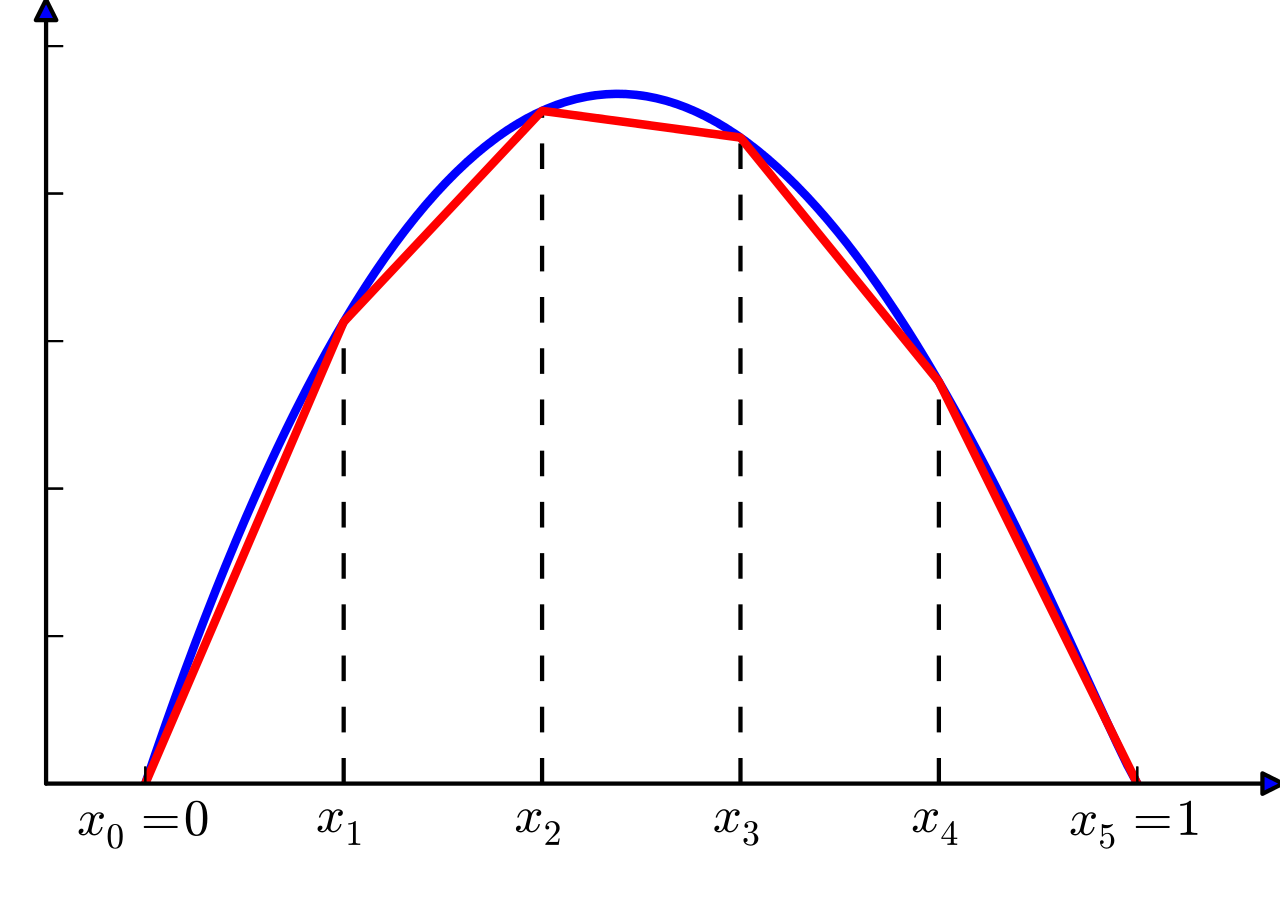
\includegraphics[width = 0.8\linewidth]{title_image}
	\end{center}
\end{figure}

\vspace{80pt}

\newpage

\tableofcontents

\newpage

\section{Model Problems}

\subsection{Diffusion Equation}

The \textit{first} model second-order linear ordinary differential equation boundary-value problem consists of:
\begin{itemize}
	\item the second-order linear ordinary differential equation:
	\begin{equation}
	-u''(x)+k^2u(x)=k^2x \qquad x \in (0, 1)
	\end{equation}
	\item the boundary conditions:
	\begin{equation}
	u(0) = 0 \quad \textnormal{and} \quad u(1) = 0 
	\end{equation}
\end{itemize}
The physical model of the second-order linear ordinary differential equation boundary-value problem is that of (1) the temperature of a bar for uniaxial heat conduction, and (2) the deflection of a beam for uniaxial deformation with distributed elastic restraint.


\subsection{Harmonic Wave Equation}

The \textit{second} model second-order linear ordinary differential equation boundary-value problem consists of:
\begin{itemize}
	\item the second-order linear ordinary differential equation:
	\begin{equation}
	u''(x)+k^2u(x)=k^2x \qquad x \in (0, 1)
	\end{equation}
	\item the boundary conditions:
	\begin{equation}
	u(0) = 0 \quad \textnormal{and} \quad u(1) = 0 
	\end{equation}
\end{itemize}
The physical model of the second-order linear ordinary differential equation boundary-value problem is that of the amplitude of standing waves for uniaxial forced vibration of a bar.

\subsection{Convection-Diffusion Equation}

The \textit{third} model second-order linear ordinary differential equation boundary-value problem consists of:
\begin{itemize}
	\item the second-order linear ordinary differential equation:
	\begin{equation}
	- u''(x)+cu'(x)=0 \qquad x \in (0, 1)
	\end{equation}
	\item the boundary conditions:
	\begin{equation}
	u(0) = 0 \quad \textnormal{and} \quad u(1) = 1 
	\end{equation}
\end{itemize}
The physical model of the second-order linear ordinary differential equation boundary-value problem is that of the concentration of a flow property that convects and diffuses proportional to the constant $c$. For example, the convection-diffusion equation could represent the concentration of ink as a function of distance in a quasi-one-dimensional flow.

\newpage

\section{Analytical Solutions}

\subsection{Analytical Solution of the Diffusion Equation}

The following equation is the diffusion equation.
\begin{equation}
-u''(x)+k^2u(x)=k^2x
\end{equation}

\subsubsection{Homogeneous Solution}

Let the homogeneous solution to the diffusion equation be defined as $u_h(x)$. Then, $u_h(x)$ must satisfy the following homogeneous ODE.
\begin{equation}
-u''_h(x) + k^2u_h(x) = 0
\end{equation}
The solution of the homogeneous ODE is assumed to be of the form: 
\begin{equation}
u_h(x) = e^{\lambda x}
\end{equation}
Taking the second-derivative of $u_h(x)$, substituting the second-derivative into the homogeneous ODE, and reducing the equation yields the \textbf{characteristic equation}.
\begin{equation}
u''_h = \lambda^2 e^{\lambda x}
\end{equation}
\begin{equation}
-\lambda^2 e^{\lambda x} + k^2e^{\lambda x} = 0
\end{equation}
\begin{equation}
\mathbf{-\lambda^2 + k^2 = 0}
\end{equation}
Solving for $\lambda$ yields:
\begin{equation}
\lambda = \pm k
\end{equation}
The homogenous solution $u_h(x)$ is then:
\begin{equation}
u_h(x) = \alpha e^{kx} + \beta e^{-kx}
\end{equation}
By making a transformation with the following relations, a more sophistocated solution can be developed:
\begin{equation}
\gamma = \frac{\alpha+\beta}{2} \quad \textnormal{and} \quad \delta = \frac{\alpha-\beta}{2}
\end{equation}
\begin{equation}
u_h(x) = \gamma \frac{e^{kx}+e^{-kx}}{2} + \delta \frac{e^{kx}-e^{-kx}}{2}
\end{equation}
\begin{equation}
\mathbf{u_h(x) = \gamma cosh(kx) + \delta sinh(kx)}
\end{equation}

\subsubsection{Particular Solution}

Let the particular solution to the diffusion equation be defined as $u_p(x)$. Then, $u_p(x)$ must satisfy the ODE:
\begin{equation}
-u''_p(x) + k^2u_p(x) = k^2x
\end{equation}
The second-derivative of $u_p(x)$, $u''_p(x)$, is assumed to be zero, and thus yields the particular solution $u_p(x)$:
\begin{equation}
k^2u_p(x) = k^2x
\end{equation}
\begin{equation}
\mathbf{u_p(x) = x}
\end{equation}

\subsubsection{Application of Boundary Conditions}

Given that $u_h(x)$ is a solution to the homogeneous ODE and $u_p(x)$ is a solution to the ODE, then the combination of $u_h(x)$ and $u_p(x)$ is also a solution to the ODE.
\begin{equation}
u(x) = u_h(x) + u_p(x)
\end{equation}
\begin{equation}
u(x) = \gamma \cosh(kx) + \delta \sinh(kx) + x
\end{equation}
The boundary conditions for the model problem are:
\begin{equation}
u(0) = 0 \quad \textnormal{and} \quad u(1) = 0 
\end{equation}
Applying the first boundary condition, $u(0) = 0$, we get that $\gamma = 0$:
\begin{equation}
u(0) = 0 = \gamma \cosh(0) + \delta \sinh(0) + 0
\end{equation}
\begin{equation}
\gamma = 0
\end{equation}
Applying the second boundary condition, $u(1) = 0$, we get that $\delta = \frac{-1}{\sinh(k)}$:
\begin{equation}
u(1) = 0 = \delta \sinh(k) + 1
\end{equation}
\begin{equation}
\delta = \frac{-1}{\sinh(k)}
\end{equation}

\subsubsection{Analytical Solution}

Thus, it is shown that for the negative second-order linear ordinary differential equation with specified boundary conditions (reproduced below) that $u(x)$ is a solution to the differential equation on $x \in (0, 1)$.
\begin{equation}
-u''(x)+k^2u(x)=k^2x \qquad x \in (0, 1)
\end{equation}
\begin{equation}
u(0) = 0 \quad \textnormal{and} \quad u(1) = 0 
\end{equation}
\begin{equation}
\mathbf{u(x) = x - \frac{sinh(kx)}{sinh(k)}}
\end{equation}

The values of $k$ tested in this study were $k \in {1, 2, 5, 10, 20, 50}$. A plot of the analytical solution for values of $k$ is depicted in Figure \ref{fig:analytical_diff}:
\begin{figure}[H]
	\begin{center}
		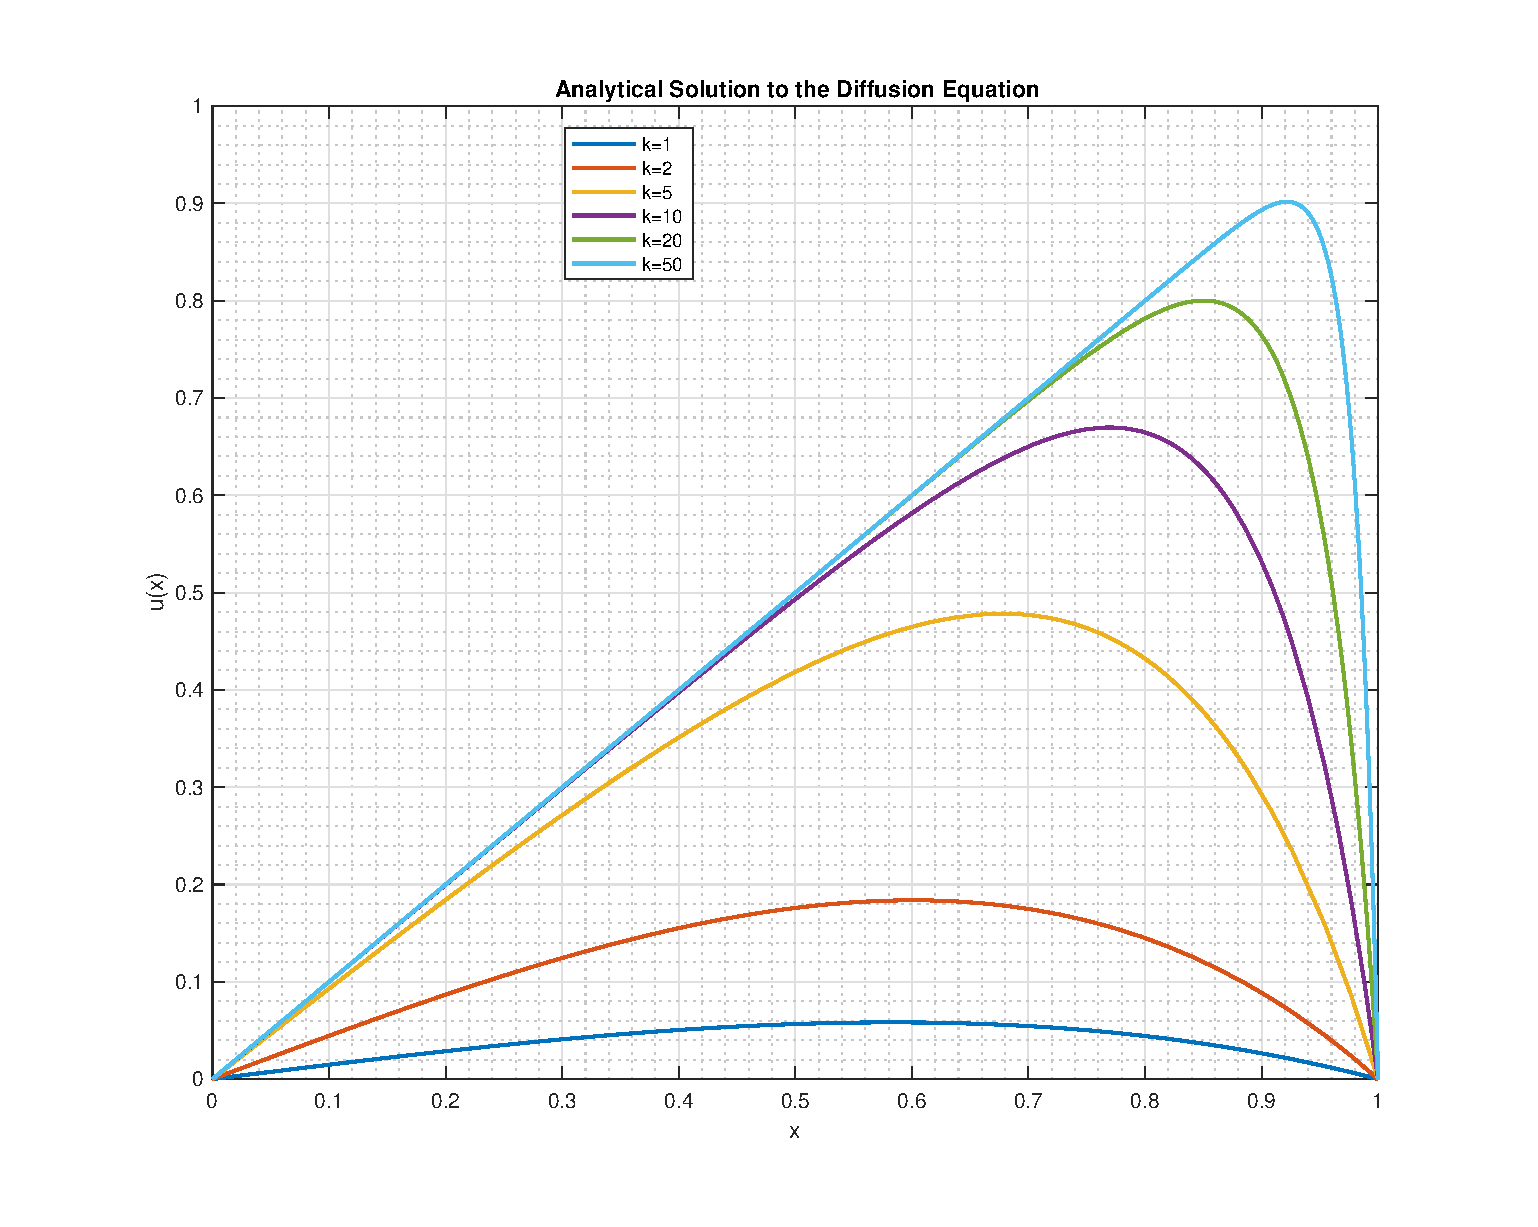
\includegraphics[width = 0.9\linewidth]{analytical_solution_diffusion}
		\caption{Analytical Solution to the Diffusion Equation for Values of $k$}
		\label{fig:analytical_diff}
	\end{center}
\end{figure}

\newpage

\subsection{Analytical Solution of the Harmonic Wave Equation}

The following equation is the harmonic wave equation.
\begin{equation}
u''(x)+k^2u(x)=k^2x
\end{equation}

\subsubsection{Homogeneous Solution}

Let the homogeneous solution to the harmonic wave equation be defined as $u_h(x)$. Then, $u_h(x)$ must satisfy the following homogeneous ODE.
\begin{equation}
u''_h(x) + k^2u_h(x) = 0
\end{equation}
The solution of the homogeneous ODE is assumed to be of the form: 
\begin{equation}
u_h(x) = e^{\lambda x}
\end{equation}
Taking the second-derivative of $u_h(x)$, substituting the second-derivative into the homogeneous ODE, and reducing the equation yields the \textbf{characteristic equation}.
\begin{equation}
u''_h(x) = \lambda^2 e^{\lambda x}
\end{equation}
\begin{equation}
\lambda^2 e^{\lambda x} + k^2e^{\lambda x} = 0
\end{equation}
\begin{equation}
\mathbf{\lambda^2 + k^2 = 0}
\end{equation}
Solving for $\lambda$ yields:
\begin{equation}
\lambda = \pm ik
\end{equation}
The homogenous solution $u_h(x)$ is then:
\begin{equation}
u_h(x) = \alpha e^{ikx} + \beta e^{-ikx}
\end{equation}
Making a transformation with the following relations, a more sophistocated solution can be developed:
\begin{equation}
\gamma = \frac{\alpha+\beta}{2} \quad \textnormal{and} \quad \delta = i\frac{\alpha-\beta}{2}
\end{equation}
\begin{equation}
u_h(x) = \gamma \frac{e^{ikx}+e^{-ikx}}{2} + \delta \frac{e^{ikx}-e^{-ikx}}{2i}
\end{equation}
\begin{equation}
\mathbf{u_h(x) = \gamma cos(kx) + \delta sin(kx)}
\end{equation}

\subsubsection{Particular Solution}

Let the particular solution to the harmonic wave equation be defined as $u_p(x)$. Then, $u_p(x)$ must satisfy the ODE:
\begin{equation}
u''_p(x) + k^2u_p(x) = k^2x
\end{equation}
The second-derivative of $u_p(x)$, $u''_p(x)$, is assumed to be zero, and thus yields the particular solution $u_p(x)$:
\begin{equation}
k^2u_p(x) = k^2x
\end{equation}
\begin{equation}
\mathbf{u_p(x) = x}
\end{equation}

\subsubsection{Application of Boundary Conditions}

Given that $u_h(x)$ is a solution to the homogeneous ODE and $u_p(x)$ is a solution to the ODE, then the combination of $u_h(x)$ and $u_p(x)$ is also a solution to the ODE.
\begin{equation}
u(x) = u_h(x) + u_p(x)
\end{equation}
\begin{equation}
u(x) = \gamma \cos(kx) + \delta \sin(kx) + x
\end{equation}
The boundary conditions for the model problem are:
\begin{equation}
u(0) = 0 \quad \textnormal{and} \quad u(1) = 0 
\end{equation}
Applying the first boundary condition, $u(0) = 0$, we get that $\gamma = 0$:
\begin{equation}
u(0) = 0 = \gamma \cos(0) + \delta \sin(0) + 0
\end{equation}
\begin{equation}
\gamma = 0
\end{equation}
Applying the second boundary condition, $u(1) = 0$, we get that $\delta = \frac{-1}{\sin(k)}$:
\begin{equation}
u(1) = 0 = \delta \sin(k) + 1
\end{equation}
\begin{equation}
\delta = \frac{-1}{\sin(k)}
\end{equation}

\subsubsection{Analytical Solution}

Thus, it is shown that for the positive second-order linear ordinary differential equation with specified boundary conditions (reproduced below) that $u(x)$ is a solution to the differential equation on $x \in (0, 1)$.
\begin{equation}
u''(x)+k^2u(x)=k^2x \qquad x \in (0, 1)
\end{equation}
\begin{equation}
u(0) = 0 \quad \textnormal{and} \quad u(1) = 0 
\end{equation}
\begin{equation}
\mathbf{u(x) = x - \frac{sin(kx)}{sin(k)}}
\end{equation}

The values of $k$ tested in this study were $k \in {1, 2, 5, 10, 20, 50}$. A plot of the analytical solution for values of $k$ is depicted in Figure \ref{fig:analytical_harmonic}:
\begin{figure}[H]
	\begin{center}
		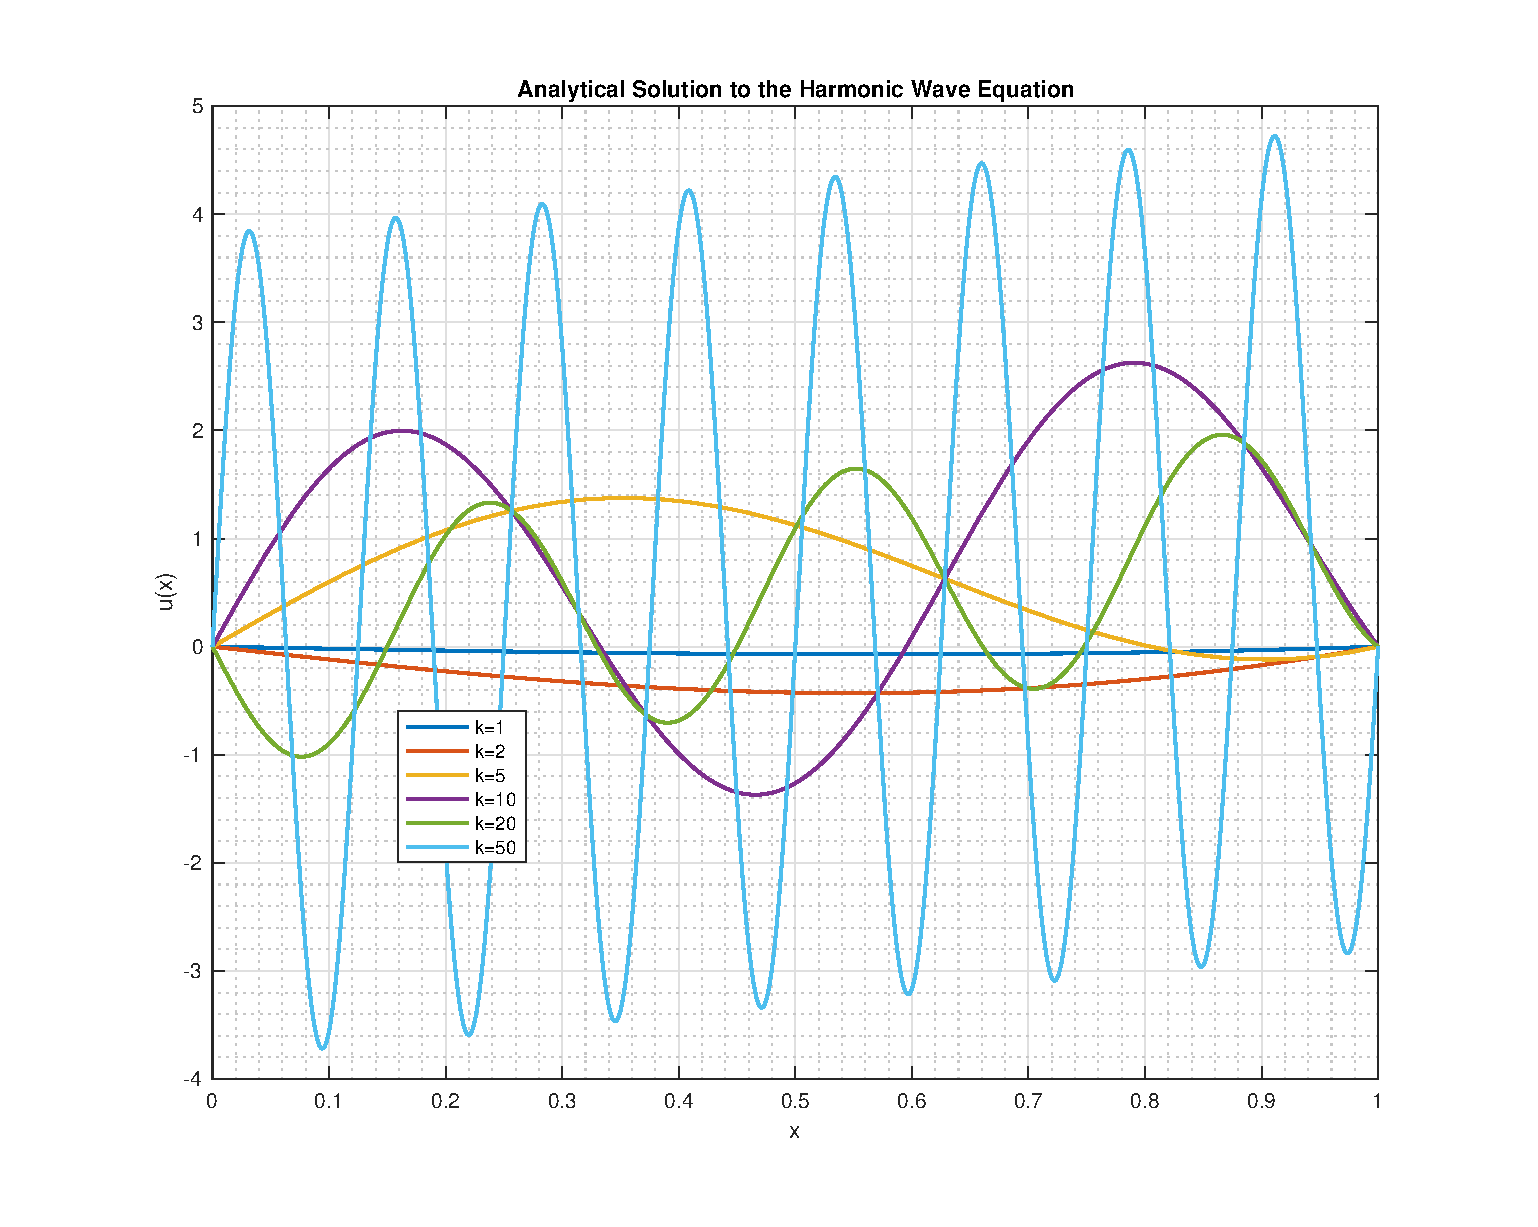
\includegraphics[width = 0.9\linewidth]{analytical_solution_harmonic_wave}
		\caption{Analytical Solution to the Harmonic Wave Equation for Values of $k$}
		\label{fig:analytical_harmonic}
	\end{center}
\end{figure}

\newpage

\subsection{Analytical Solution of the Convection-Diffusion Equation}

The following equation is the homogeneous second-order linear ordinary differential equation (ODE).
\begin{equation}
- u''(x)+cu'(x)=0
\end{equation}

\subsubsection{Homogeneous Solution}

The solution of the homogeneous ODE, $u_h(x)$ is assumed to be of the form: 
\begin{equation}
u_h(x) = e^{\lambda x}
\end{equation}
Taking the derivatives of $u_h(x)$, substituting them into the homogeneous ODE, and reducing the equation yields the \textbf{characteristic equation}.
\begin{equation}
u'_h(x) = \lambda e^{\lambda x}
\end{equation}
\begin{equation}
u''_h(x) = \lambda^2 e^{\lambda x}
\end{equation}
\begin{equation}
-\lambda^2 e^{\lambda x} + c \lambda e^{\lambda x} = 0
\end{equation}
\begin{equation}
\mathbf{-\lambda^2 + c \lambda = \lambda(c-\lambda) = 0}
\end{equation}
Solving for $\lambda$ yields:
\begin{equation}
\lambda = \{0, c\}
\end{equation}
The homogenous solution $u_h(x)$ is then:
\begin{equation}
u_h(x) = ae^{0x} + be^{cx} 
\end{equation}
\begin{equation}
\mathbf{u_h(x) = a + be^{cx}}
\end{equation}

\subsubsection{Application of Boundary Conditions}

Applying the both boundary conditions, $u(0) = 0$ and $u(1) = 1$, we get the system of algebraic equations, which yields $a$ and $b$:
\begin{equation}
u_h(0) = 0 = a + b
\end{equation}
\begin{equation}
u_h(1) = 1 = a + be^c
\end{equation}
\begin{equation}
	\begin{bmatrix}
		1 & 1 \\ 1 & e^c
	\end{bmatrix}
	\begin{bmatrix}
	a \\ b
	\end{bmatrix}
	=
	\begin{bmatrix}
	0 \\ 1
	\end{bmatrix}
\end{equation}
\begin{equation}
a = \frac{-1}{e^c-1} \quad \textnormal{and} \quad b = \frac{1}{e^c-1}
\end{equation}

\subsubsection{Analytical Solution}

Thus, it is shown that for the second-order linear ordinary differential equation with specified boundary conditions, that $u(x)$ is a solution to the differential equation on $x \in (0, 1)$.
\begin{equation}
-u''(x)+cu'(x)=0 \qquad x \in (0, 1)
\end{equation}
\begin{equation}
u(0) = 0 \quad \textnormal{and} \quad u(1) = 1 
\end{equation}
\begin{equation}
\mathbf{u(x) = \frac{e^{cx}-1}{e^c-1}}
\end{equation}

The values of $c$ tested in this study were $c \in {1, 2, 5, 10, 20, 50}$. A plot of the analytical solution for values of $c$ is depicted in Figure \ref{fig:analytical_conv_diff}:
\begin{figure}[H]
	\begin{center}
		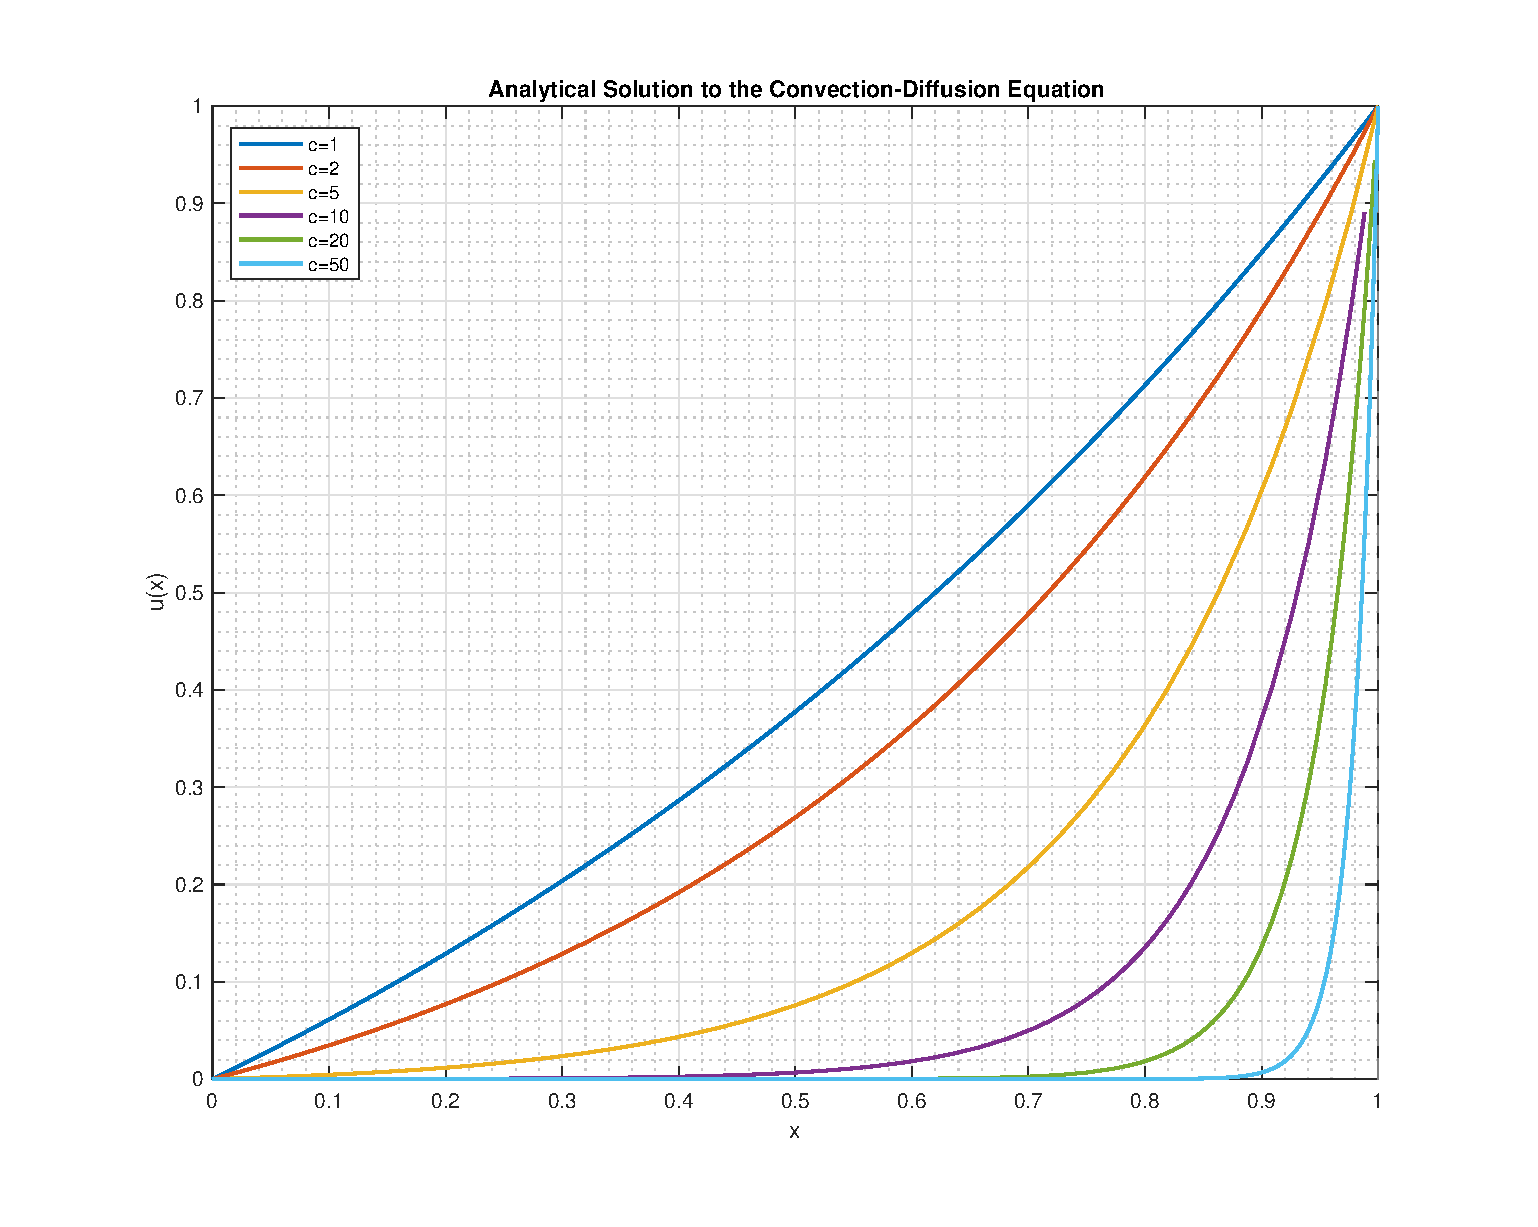
\includegraphics[width = 0.9\linewidth]{analytical_solution_convection_diffusion}
		\caption{Analytical Solution to the Convection-Diffusion Equation for Values of $c$}
		\label{fig:analytical_conv_diff}
	\end{center}
\end{figure}

\newpage

\subsection{Analytical Solution of the Quantity of Interest for the Diffusion Equation}

The quantity of interest for the diffusion equation is the first derivative at the right boundary, or $u'(1)$. The differential equation and the analytical solution to the differential equation, respectively, are reproduced below.
\begin{equation}
-u''(x)+k^2u(x)=k^2x
\end{equation}
\begin{equation}
u(x) = x - \frac{\sinh(kx)}{\sinh(k)}
\end{equation}
Thus, taking the first derivative, and solving at $x = 1$, we obtain the exact quantity of interest:
\begin{equation}
u'(x) = 1 - \frac{k\cosh(kx)}{\sinh(k)}
\end{equation}
\begin{equation}
u'(1) = 1 - \frac{k\cosh(k)}{\sinh(k)}
\end{equation}
\begin{equation}
\mathbf{u'(1) = 1 - kcoth(k)}
\end{equation}
As $k$ approaches 0, the quantity of interest approaches 0. As $k$ approaches $\infty$, $\coth(x)$ approaches 1, and thus for large $k$, the quantity of interest behaves as $1-k$. Additionally, since $\coth(x)$ approaches 1 as $x$ approaches $\infty$; as $k$ approaches $\infty$, the quantity of interest approaches $\infty$:
\begin{equation}
\lim_{k\to 0} [1 - k\coth(k)] = 0
\end{equation}
\begin{equation}
\lim_{k\to\infty} [1 - k\coth(k)] \approx \lim_{k\to\infty} (1-k) = -\infty
\end{equation}

A table of the exact quantity of interest for the tested values of $k$ is included below (for $k=(20, 50)$, error is less than machine epsilon, $\epsilon$):
\begin{table}[H]
	\caption{Analytical Solution to the Quantity of Interest for the Diffusion Equation for Values of $k$}
	\begin{tabular}{|c|c|}
		\hline 
		$\mathbf{k}$ & $\mathbf{u'(1)}$ \\ 
		\hline 
		1 & -0.313035 \\ 
		\hline 
		2 & -1.074629 \\ 
		\hline 
		5 & -4.000454 \\ 
		\hline 
		10 & -9.0000000412 \\ 
		\hline 
		20 & -19.000000000000000 \\ 
		\hline 
		50 & -49.000000000000000 \\ 
		\hline 
	\end{tabular}
\end{table} 

\newpage

\subsection{Analytical Solution of the Quantity of Interest for the Harmonic Wave Equation}

The quantity of interest for the harmonic wave equation is the first derivative at the right boundary, or $u'(1)$. The differential equation and the analytical solution to the differential equation, respectively, are reproduced below.
\begin{equation}
u''(x)+k^2u(x)=k^2x
\end{equation}
\begin{equation}
u(x) = x - \frac{\sin(kx)}{\sin(k)}
\end{equation}
Thus, taking the first derivative, and solving at $x = 1$, we obtain the exact quantity of interest:
\begin{equation}
u'(x) = 1 - \frac{k\cos(kx)}{\sin(k)}
\end{equation}
\begin{equation}
u'(x) = 1 - \frac{k\cos(k)}{\sin(k)}
\end{equation}
\begin{equation}
\mathbf{u'(1) = 1 - kcot(k)}
\end{equation}
As $k$ approaches 0, the quantity of interest approaches 0. But, since $\cot(x)$ is oscillatory, the quantity of interest does not converge as $k$ approaches $\infty$:
\begin{equation}
\lim_{k\to 0} [1 - k\cot(k)] = 0
\end{equation}
\begin{equation}
\lim_{k\to\infty} [1 - k\cot(k)] = -\infty \;\; to \;\; \infty
\end{equation}

A table of the exact quantity of interest for the tested values of $k$ is included below:
\begin{table}[H]
	\caption{Analytical Solution to the Quantity of Interest for the Harmonic Wave Equation for Values of $k$}
	\begin{tabular}{|c|c|}
	\hline 
	$\mathbf{k}$ & $\mathbf{u'(1)}$ \\ 
	\hline 
	1 & 0.3579 \\ 
	\hline 
	2 & 1.9153 \\ 
	\hline 
	5 & 2.4790 \\ 
	\hline 
	10 & -14.4235 \\ 
	\hline 
	20 & -7.9399 \\ 
	\hline 
	50 & 184.8907 \\ 
	\hline 
\end{tabular}
\end{table} 

\newpage

\subsection{Analytical Solution of the Quantity of Interest for the Convection-Diffusion Equation}

The quantity of interest for the convection-diffusion equation is the first derivative at the right boundary, or $u'(1)$. The differential equation and the analytical solution to the differential equation, respectively, are reproduced below.
\begin{equation}
- u''(x)+cu'(x)=0
\end{equation}
\begin{equation}
u(x) = \frac{e^{cx}-1}{e^c-1}
\end{equation}
Thus, taking the first derivative, and solving at $x = 1$, we obtain the exact quantity of interest:
\begin{equation}
u'(x) = \frac{ce^{cx}}{e^c-1}
\end{equation}
\begin{equation}
\mathbf{u'(1) = \frac{ce^{c}}{e^c-1}}
\end{equation}
It can be seen that if $e^c$, or rather $c$, is sufficiently large ($e^c \gg 1$), then the quantity of interest tends to $c$ given that the ratio of $e^c$ and $(e^c -1)$ tends to unity:
\begin{equation}
\lim_{c\to\infty} \frac{ce^{c}}{e^c-1} = c
\end{equation}

A table of the exact quantity of interest for the tested values of $c$ is included below (for $c=50$, error is less than machine epsilon, $\epsilon$):
\begin{table}[H]
	\caption{Analytical Solution to the Quantity of Interest for the Convection-Diffusion Equation for Values of $c$}
\begin{tabular}{|c|c|}
	\hline 
	$\mathbf{c}$ & $\mathbf{u'(1)}$ \\ 
	\hline 
	1 & 1.58198 \\ 
	\hline 
	2 & 2.31304 \\ 
	\hline 
	5 & 5.03392 \\ 
	\hline 
	10 & 10.00045 \\ 
	\hline 
	20 & 20.00000004 \\ 
	\hline 
	50 & 50.00000000 \\ 
	\hline 
\end{tabular}
\end{table} 

\newpage

\section{Numerical Methods}

\subsection{Derivations for the Diffusion Equation}

\subsubsection{2nd-Order Central Difference Scheme Finite Difference Method}

\paragraph{Second Derivative}

Developing the Taylor series for $u(x)$ in the vicinity of $x = i$:
\begin{equation}
u_{i-1} = u_i - \Delta x u'_i + \frac{\Delta x^2}{2} u''_i - \frac{\Delta x^3}{6} u^{(3)}_i + \frac{\Delta x^4}{24} u^{(4)}_i + \mathcal{O}(\Delta x^5)
\end{equation}
\begin{equation}
u_{i+1} = u_i + \Delta x u'_i + \frac{\Delta x^2}{2} u''_i + \frac{\Delta x^3}{6} u^{(3)}_i + \frac{\Delta x^4}{24} u^{(4)}_i + \mathcal{O}(\Delta x^5)
\end{equation}
Adding the Taylor series for $u_{i-1}$ and $u_{i+1}$ and canceling terms:
\begin{equation}
u_{i+1} + u_{i-1} = 2u_i + \Delta x^2 u''_i + \mathcal{O}(\Delta x^4)
\end{equation}
Rearranging terms to solve for $u''_i$:
\begin{equation}
u''_i = \frac{u_{i+1} - 2u_i + u_{i-1}}{\Delta x^2} + \mathcal{O}(\Delta x^2) 
\end{equation}

From this specific second-derivative formulation using the finite difference method, the approximation can be observed to be second-order ($\mathcal{O}(\Delta x^2)$).

\paragraph{Discretized Differential Equation}

The differential equation is:
\begin{equation}
-u''(x)+k^2u(x)=k^2x
\end{equation}
Discretizing using the above formulas and simplifying yields:
\begin{equation}
\left(-1\right) u_{i-1} + \left(2 + k^2\Delta x^2\right) u_{i} + \left(-1\right) u_{i+1} = \left(k^2\Delta x^2 \right)x_i
\end{equation}

\subsubsection{4th-Order Central Difference Scheme Finite Difference Method}

\paragraph{Second Derivative}

Developing the Taylor series for $u(x)$ in the vicinity of $x = i$:
\begin{equation}
u_{i-1} = u_i - \Delta x u'_i + \frac{\Delta x^2}{2} u''_i - \frac{\Delta x^3}{6} u^{(3)}_i + \frac{\Delta x^4}{24} u^{(4)}_i + \mathcal{O}(\Delta x^5)
\end{equation}
\begin{equation}
u_{i+1} = u_i + \Delta x u'_i + \frac{\Delta x^2}{2} u''_i + \frac{\Delta x^3}{6} u^{(3)}_i + \frac{\Delta x^4}{24} u^{(4)}_i + \mathcal{O}(\Delta x^5)
\end{equation}
Adding the Taylor series for $u_{i-1}$ and $u_{i+1}$ and canceling terms:
\begin{equation}
u_{i+1} + u_{i-1} = 2u_i + \Delta x^2 u''_i + \frac{\Delta x^4}{12} u^{(4)}_i + \mathcal{O}(\Delta x^6)
\end{equation}
Rearranging for $u''_i$, we get:
\begin{equation}
u''_i = \frac{u_{i+1} -2u_i + u_{i-1}}{\Delta x^2} - \frac{\Delta x^2}{12} u^{(4)}_i + \mathcal{O}(\Delta x^4)
\end{equation}
Returning to the differential equation and then taking two additional derivatives, we can arrive at an expression for $u^{(4)}_i$:
\begin{equation}
-u''(x)+k^2u(x)=k^2x \qquad x \in (0, 1)
\end{equation}
\begin{equation}
-u^{(4)}(x)+k^2u''(x)=0
\end{equation}
\begin{equation}
u^{(4)}(x) = k^2u''(x)
\end{equation}
Substituting in the fourth-derivative expression:
\begin{equation}
u''_i = \frac{u_{i+1} -2u_i + u_{i-1}}{\Delta x^2} - \frac{\Delta x^2}{12} k^2u''_i + \mathcal{O}(\Delta x^4)
\end{equation}
Now, exchanging the $u''_i$ term with the earlier derivation and simplifying:
\begin{equation}
u''_i = \frac{u_{i+1} -2u_i + u_{i-1}}{\Delta x^2} - \frac{\Delta x^2}{12} k^2 \left[\frac{u_{i+1} -2u_i + u_{i-1}}{\Delta x^2} + \mathcal{O}(\Delta x^2) \right] + \mathcal{O}(\Delta x^4)
\end{equation}
\begin{equation}
u''_i = \frac{1}{\Delta x^2} (u_{i+1} -2u_i + u_{i-1}) - \frac{k^2}{12} (u_{i+1} -2u_i + u_{i-1}) + \mathcal{O}(\Delta x^4)
\end{equation}
\begin{equation}
u''_i = \left(\frac{1}{\Delta x^2} - \frac{k^2}{12}\right) (u_{i+1} -2u_i + u_{i-1}) + \mathcal{O}(\Delta x^4)
\end{equation}
From this specific second-derivative formulation using the finite difference method, the approximation can be observed to be fourth-order ($\mathcal{O}(\Delta x^4)$).

\paragraph{Discretized Differential Equation}

The differential equation is:
\begin{equation}
-u''(x)+k^2u(x)=k^2x
\end{equation}
Discretizing using the above formulas and simplifying yields:
\begin{equation}
\left(-1 + \frac{k^2\Delta x^2}{12}\right) u_{i-1} + \left(2 + \frac{10 k^2\Delta x^2}{12}\right) u_{i} + \left(-1+ \frac{k^2\Delta x^2}{12}\right) u_{i+1} = \left(k^2\Delta x^2 \right)x_i
\end{equation}

\subsubsection{1st-Order (p=1) Galerkin Method Finite Element Method}

\subsubsection{2nd-Order (p=2) Galerkin Method Finite Element Method}

\newpage

\subsection{Derivations for the Harmonic Wave Equation}

\subsubsection{2nd-Order Central Difference Scheme Finite Difference Method}

\paragraph{Second Derivative}

Developing the Taylor series for $u(x)$ in the vicinity of $x = i$:
\begin{equation}
u_{i-1} = u_i - \Delta x u'_i + \frac{\Delta x^2}{2} u''_i - \frac{\Delta x^3}{6} u^{(3)}_i + \frac{\Delta x^4}{24} u^{(4)}_i + \mathcal{O}(\Delta x^5)
\end{equation}
\begin{equation}
u_{i+1} = u_i + \Delta x u'_i + \frac{\Delta x^2}{2} u''_i + \frac{\Delta x^3}{6} u^{(3)}_i + \frac{\Delta x^4}{24} u^{(4)}_i + \mathcal{O}(\Delta x^5)
\end{equation}
Adding the Taylor series for $u_{i-1}$ and $u_{i+1}$ and canceling terms:
\begin{equation}
u_{i+1} + u_{i-1} = 2u_i + \Delta x^2 u''_i + \mathcal{O}(\Delta x^4)
\end{equation}
Rearranging terms to solve for $u''_i$:
\begin{equation}
u''_i = \frac{u_{i+1} - 2u_i + u_{i-1}}{\Delta x^2} + \mathcal{O}(\Delta x^2) 
\end{equation}

From this specific second-derivative formulation using the finite difference method, the approximation can be observed to be second-order ($\mathcal{O}(\Delta x^2)$).

\paragraph{Discretized Differential Equation}

The differential equation is:
\begin{equation}
u''(x)+k^2u(x)=k^2x
\end{equation}
Discretizing using the above formulas and simplifying yields:
\begin{equation}
\left(1\right) u_{i-1} + \left(-2 + k^2\Delta x^2\right) u_{i} + \left(1\right) u_{i+1} = \left(k^2\Delta x^2 \right)x_i
\end{equation}

\subsubsection{4th-Order Central Difference Scheme Finite Difference Method}

\paragraph{Second Derivative}

Developing the Taylor series for $u(x)$ in the vicinity of $x = i$:
\begin{equation}
u_{i-1} = u_i - \Delta x u'_i + \frac{\Delta x^2}{2} u''_i - \frac{\Delta x^3}{6} u^{(3)}_i + \frac{\Delta x^4}{24} u^{(4)}_i + \mathcal{O}(\Delta x^5)
\end{equation}
\begin{equation}
u_{i+1} = u_i + \Delta x u'_i + \frac{\Delta x^2}{2} u''_i + \frac{\Delta x^3}{6} u^{(3)}_i + \frac{\Delta x^4}{24} u^{(4)}_i + \mathcal{O}(\Delta x^5)
\end{equation}
Adding the Taylor series for $u_{i-1}$ and $u_{i+1}$ and canceling terms:
\begin{equation}
u_{i+1} + u_{i-1} = 2u_i + \Delta x^2 u''_i + \frac{\Delta x^4}{12} u^{(4)}_i + \mathcal{O}(\Delta x^6)
\end{equation}
Rearranging for $u''_i$, we get:
\begin{equation}
u''_i = \frac{u_{i+1} -2u_i + u_{i-1}}{\Delta x^2} - \frac{\Delta x^2}{12} u^{(4)}_i + \mathcal{O}(\Delta x^4)
\end{equation}
Returning to the differential equation and then taking two additional derivatives, we can arrive at an expression for $u^{(4)}_i$:
\begin{equation}
u''(x)+k^2u(x)=k^2x \qquad x \in (0, 1)
\end{equation}
\begin{equation}
u^{(4)}(x)+k^2u''(x)=0
\end{equation}
\begin{equation}
u^{(4)}(x) = - k^2u''(x)
\end{equation}
Substituting in the fourth-derivative expression:
\begin{equation}
u''_i = \frac{u_{i+1} -2u_i + u_{i-1}}{\Delta x^2} + \frac{\Delta x^2}{12} k^2u''_i + \mathcal{O}(\Delta x^4)
\end{equation}
Now, exchanging the $u''_i$ term with the earlier derivation and simplifying:
\begin{equation}
u''_i = \frac{u_{i+1} -2u_i + u_{i-1}}{\Delta x^2} + \frac{\Delta x^2}{12} k^2 \left[\frac{u_{i+1} -2u_i + u_{i-1}}{\Delta x^2} + \mathcal{O}(\Delta x^2) \right] + \mathcal{O}(\Delta x^4)
\end{equation}
\begin{equation}
u''_i = \frac{1}{\Delta x^2} (u_{i+1} -2u_i + u_{i-1}) + \frac{k^2}{12} (u_{i+1} -2u_i + u_{i-1}) + \mathcal{O}(\Delta x^4)
\end{equation}
\begin{equation}
u''_i = \left(\frac{1}{\Delta x^2} + \frac{k^2}{12}\right) (u_{i+1} -2u_i + u_{i-1}) + \mathcal{O}(\Delta x^4)
\end{equation}
From this specific second-derivative formulation using the finite difference method, the approximation can be observed to be fourth-order ($\mathcal{O}(\Delta x^4)$).

\paragraph{Discretized Differential Equation}

The differential equation is:
\begin{equation}
u''(x)+k^2u(x)=k^2x
\end{equation}
Discretizing using the above formulas and simplifying yields:
\begin{equation}
\left(1 + \frac{k^2\Delta x^2}{12}\right) u_{i-1} + \left(-2 + \frac{10 k^2\Delta x^2}{12}\right) u_{i} + \left(1+ \frac{k^2\Delta x^2}{12}\right) u_{i+1} = \left(k^2\Delta x^2 \right)x_i
\end{equation}

\subsubsection{ 1st-Order (p=1) Galerkin Method Finite Element Method}

\subsubsection{ 2nd-Order (p=2) Galerkin Method Finite Element Method}

\newpage

\subsection{Derivations for the Convection-Diffusion Equation}

\subsubsection{2nd-Order Central Difference Scheme Finite Difference Method}

\paragraph{First Derivative}
Developing the Taylor series for $u(x)$ in the vicinity of $x = i$:
\begin{equation}
u_{i-1} = u_i - \Delta x u'_i + \frac{\Delta x^2}{2} u''_i - \frac{\Delta x^3}{6} u^{(3)}_i + \frac{\Delta x^4}{24} u^{(4)}_i + \mathcal{O}(\Delta x^5)
\end{equation}
\begin{equation}
u_{i+1} = u_i + \Delta x u'_i + \frac{\Delta x^2}{2} u''_i + \frac{\Delta x^3}{6} u^{(3)}_i + \frac{\Delta x^4}{24} u^{(4)}_i + \mathcal{O}(\Delta x^5)
\end{equation}
Subtracting the Taylor series for $u_{i-1}$ from $u_{i+1}$ and canceling terms:
\begin{equation}
u_{i+1} - u_{i-1} = 2\Delta xu'_i + \frac{\Delta x^3}{3} u^{(3)}_i + \mathcal{O}(\Delta x^5)
\end{equation}
Solving for $u'_i$:
\begin{equation}
u'_i = \frac{u_{i+1} - u_{i-1}}{2 \Delta x} + \mathcal{O}(\Delta x^2) 
\end{equation}

From this specific first-derivative formulation using the finite difference method, the first-derivative approximation can be observed to be second-order ($\mathcal{O}(\Delta x^2)$).

\paragraph{Second Derivative}
Developing the Taylor series for $u(x)$ in the vicinity of $x = i$:
\begin{equation}
u_{i-1} = u_i - \Delta x u'_i + \frac{\Delta x^2}{2} u''_i - \frac{\Delta x^3}{6} u^{(3)}_i + \frac{\Delta x^4}{24} u^{(4)}_i + \mathcal{O}(\Delta x^5)
\end{equation}
\begin{equation}
u_{i+1} = u_i + \Delta x u'_i + \frac{\Delta x^2}{2} u''_i + \frac{\Delta x^3}{6} u^{(3)}_i + \frac{\Delta x^4}{24} u^{(4)}_i + \mathcal{O}(\Delta x^5)
\end{equation}
Adding the Taylor series for $u_{i-1}$ and $u_{i+1}$ and canceling terms:
\begin{equation}
u_{i+1} + u_{i-1} = 2u_i + \Delta x^2 u''_i + \mathcal{O}(\Delta x^4)
\end{equation}
Rearranging terms to solve for $u''_i$:
\begin{equation}
u''_i = \frac{u_{i+1} - 2u_i + u_{i-1}}{\Delta x^2} + \mathcal{O}(\Delta x^2) 
\end{equation}

From this specific second-derivative formulation using the finite difference method, the second-derivative approximation can be observed to be second-order ($\mathcal{O}(\Delta x^2)$).

\paragraph{Discretized Differential Equation}
The differential equation is:
\begin{equation}
- u''(x)+cu'(x)=0
\end{equation}
Discretizing using the above formulas and simplifying yields:
\begin{equation}
-\left(\frac{u_{i+1} - 2u_i + u_{i-1}}{\Delta x^2}\right) + c\left(\frac{u_{i+1} - u_{i-1}}{2 \Delta x}\right) = 0
\end{equation}
\begin{equation}
-\left(u_{i+1} - 2u_i + u_{i-1}\right) + c\Delta x\left( \frac{u_{i+1} - u_{i-1}}{2}\right) = 0
\end{equation}
\begin{equation}
\left(-1-\frac{c\Delta x}{2}\right)u_{i-1} + \left(2\right)u_{i} + \left(-1+\frac{c\Delta x}{2}\right)u_{i+1} = 0
\end{equation}

\subsubsection{4th-Order Central Difference Scheme Finite Difference Method}

\paragraph{First Derivative}
Developing the Taylor series for $u(x)$ in the vicinity of $x = i$:
\begin{equation}
u_{i-1} = u_i - \Delta x u'_i + \frac{\Delta x^2}{2} u''_i - \frac{\Delta x^3}{6} u^{(3)}_i + \frac{\Delta x^4}{24} u^{(4)}_i + \mathcal{O}(\Delta x^5)
\end{equation}
\begin{equation}
u_{i+1} = u_i + \Delta x u'_i + \frac{\Delta x^2}{2} u''_i + \frac{\Delta x^3}{6} u^{(3)}_i + \frac{\Delta x^4}{24} u^{(4)}_i + \mathcal{O}(\Delta x^5)
\end{equation}
Subtracting the Taylor series for $u_{i-1}$ from $u_{i+1}$ and canceling terms:
\begin{equation}
u_{i+1} - u_{i-1} = 2\Delta xu'_i + \frac{\Delta x^3}{3} u^{(3)}_i + \mathcal{O}(\Delta x^5)
\end{equation}
Returning to the differential equation and taking one additional derivative:
\begin{equation}
u''(x)=cu'(x)
\end{equation}
\begin{equation}
u^{(3)}(x)=cu''(x)
\end{equation}
Replacing the second-derivative term with the original differential equation:
\begin{equation}
u^{(3)}(x) = c^2u'(x)
\end{equation}
Now replacing the third-derivative term in the Taylor series subtraction and then dividing by $2\Delta x$:
\begin{equation}
u_{i+1} - u_{i-1} = 2\Delta xu'_i + \frac{c^2\Delta x^3}{3}u'_i  + \mathcal{O}(\Delta x^5)
\end{equation}
\begin{equation}
\frac{u_{i+1} - u_{i-1}}{2\Delta x} = \left(1 + \frac{c^2\Delta x^2}{6}\right)u'_i  + \mathcal{O}(\Delta x^4)
\end{equation}
Solving for $u'_i$:
\begin{equation}
u'_i = \left(1 + \frac{c^2\Delta x^2}{6}\right)^{-1} \frac{u_{i+1} - u_{i-1}}{2\Delta x} + \mathcal{O}(\Delta x^4)
\end{equation}

From this specific first-derivative formulation using the finite difference method, the first-derivative approximation can be observed to be fourth-order ($\mathcal{O}(\Delta x^4)$).

\paragraph{Second Derivative}
Developing the Taylor series for $u(x)$ in the vicinity of $x = i$:
\begin{equation}
u_{i-1} = u_i - \Delta x u'_i + \frac{\Delta x^2}{2} u''_i - \frac{\Delta x^3}{6} u^{(3)}_i + \frac{\Delta x^4}{24} u^{(4)}_i + \mathcal{O}(\Delta x^5)
\end{equation}
\begin{equation}
u_{i+1} = u_i + \Delta x u'_i + \frac{\Delta x^2}{2} u''_i + \frac{\Delta x^3}{6} u^{(3)}_i + \frac{\Delta x^4}{24} u^{(4)}_i + \mathcal{O}(\Delta x^5)
\end{equation}
Adding the Taylor series for $u_{i-1}$ and $u_{i+1}$ and canceling terms:
\begin{equation}
u_{i+1} + u_{i-1} = 2u_i + \Delta x^2 u''_i + \frac{\Delta x^4}{12} u^{(4)}_i + \mathcal{O}(\Delta x^6)
\end{equation}
Returning to the differential equation and taking two additional derivatives:
\begin{equation}
u''(x)=cu'(x)
\end{equation}
\begin{equation}
u^{(3)}(x)=cu''(x)
\end{equation}
\begin{equation}
u^{(4)}(x)=cu^{(3)}(x)
\end{equation}
Replacing the fourth-derivative and third-derivative terms with the original differential equation, we arrive at:
\begin{equation}
u^{(4)}(x) = c^2u''(x)
\end{equation}
Now replacing the fourth-derivative term in the Taylor series addition, rearranging, and dividing by $\Delta x^2$:
\begin{equation}
u_{i+1} + u_{i-1} = 2u_i + \Delta x^2 u''_i + \frac{c^2\Delta x^4}{12} u''_i + \mathcal{O}(\Delta x^6)
\end{equation}
\begin{equation}
\frac{u_{i+1} -2u_i + u_{i-1}}{\Delta x^2} =  \left(1 + \frac{c^2\Delta x^2}{12} \right)u''_i + \mathcal{O}(\Delta x^4)
\end{equation}
Rearranging terms to solve for $u''_i$:
\begin{equation}
u''_i = \left(1 + \frac{c^2\Delta x^2}{12} \right)^{-1} \frac{u_{i+1} -2u_i + u_{i-1}}{\Delta x^2} + \mathcal{O}(\Delta x^4)
\end{equation}

From this specific second-derivative formulation using the finite difference method, the second-derivative approximation can be observed to be fourth-order ($\mathcal{O}(\Delta x^4)$).

\paragraph{Discretized Differential Equation}
The differential equation is:
\begin{equation}
- u''(x)+cu'(x)=0
\end{equation}
Discretizing using the above formulas and simplifying yields:
\begin{equation}
-\left(1 + \frac{c^2\Delta x^2}{12} \right)^{-1} \frac{u_{i+1} -2u_i + u_{i-1}}{\Delta x^2} + c\left(1 + \frac{c^2\Delta x^2}{6}\right)^{-1} \frac{u_{i+1} - u_{i-1}}{2\Delta x} = 0
\end{equation}
\begin{equation}
\left(-1-\frac{c\Delta x}{2}-\frac{c^2\Delta x^2}{12}\right)u_{i-1} + \left(2+\frac{c^2\Delta x^2}{6}\right)u_{i} + \left(-1+\frac{c\Delta x}{2}-\frac{c^2\Delta x^2}{12}\right)u_{i+1} = 0
\end{equation}

\subsubsection{1st-Order (p=1) Galerkin Method Finite Element Method}

\subsubsection{2nd-Order (p=2) Galerkin Method Finite Element Method}

\newpage

\section{Results}

\subsection{Finite Difference Method -- Solution Results}

\subsubsection{2nd-Order Central Difference Scheme - Diffusion Equation}

\begin{figure}[H]
	\begin{center}
		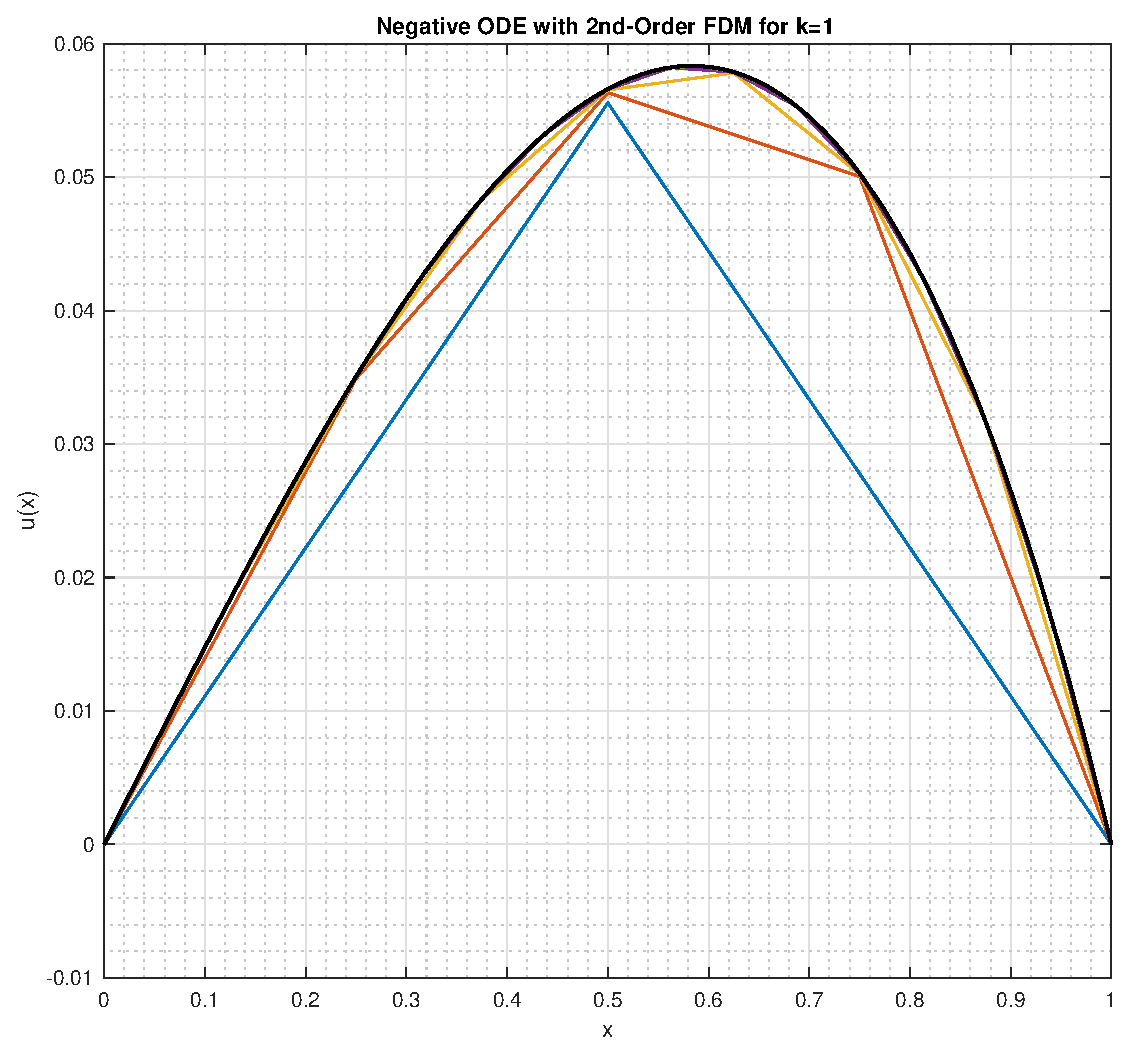
\includegraphics[width = 0.31\linewidth]{negative_ode_order_2_k_1}
		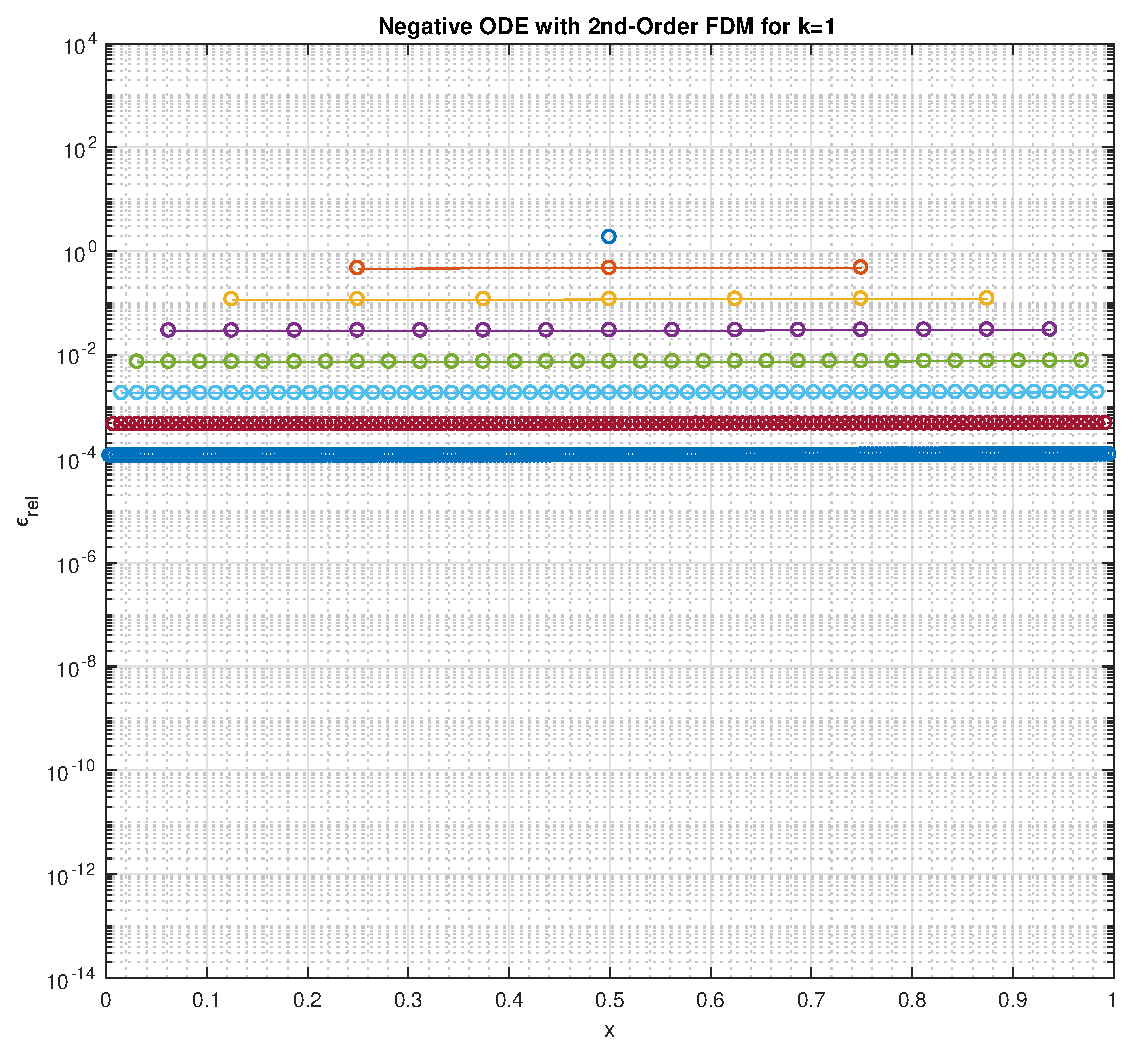
\includegraphics[width = 0.31\linewidth]{error_negative_ode_order_2_k_1}
		\caption{2nd-Order CDS FDM and Pointwise Error for Diffusion Equation with $k = 1$}
	\end{center}
\end{figure}

\begin{figure}[H]
	\begin{center}
		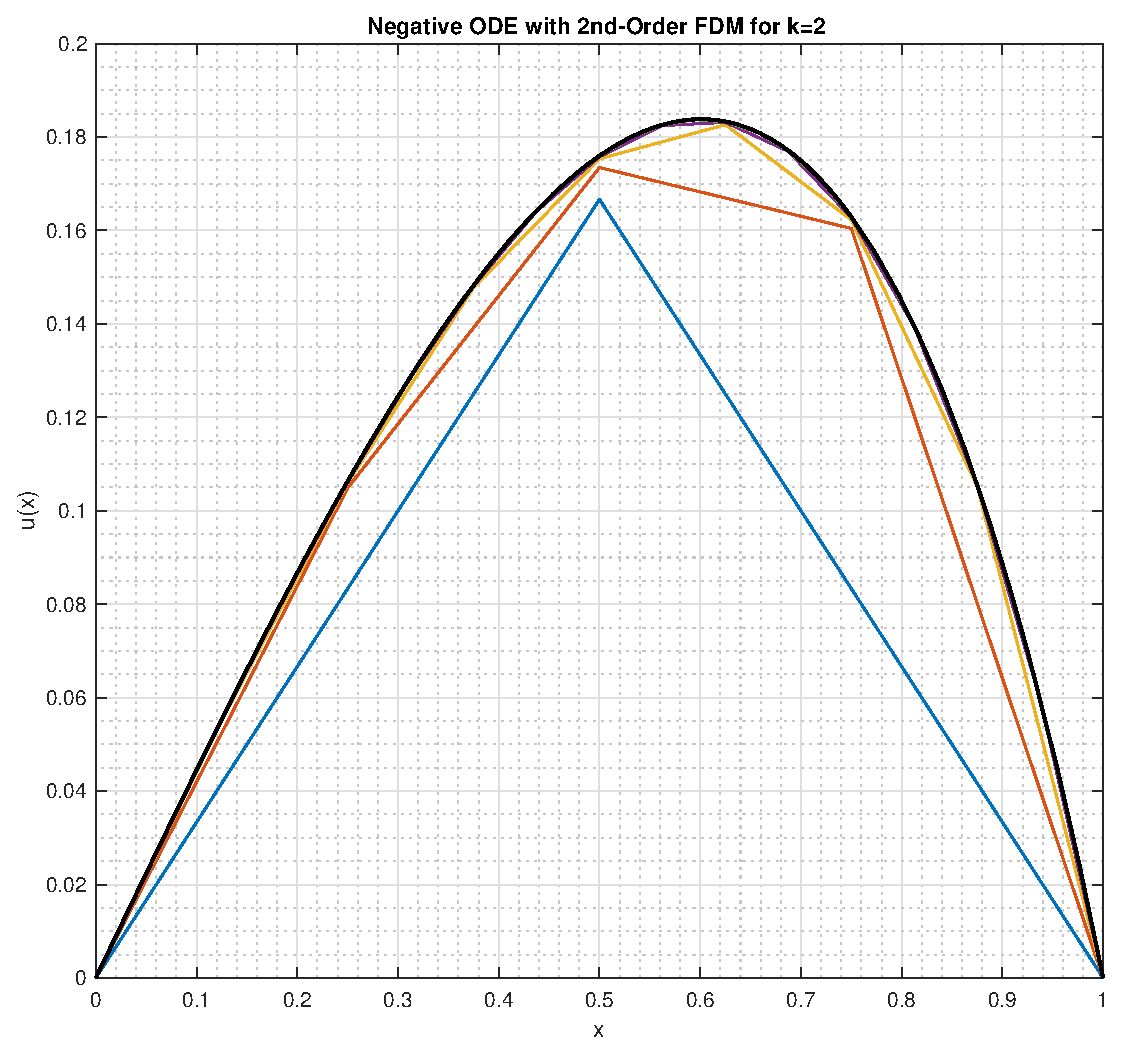
\includegraphics[width = 0.31\linewidth]{negative_ode_order_2_k_2}
		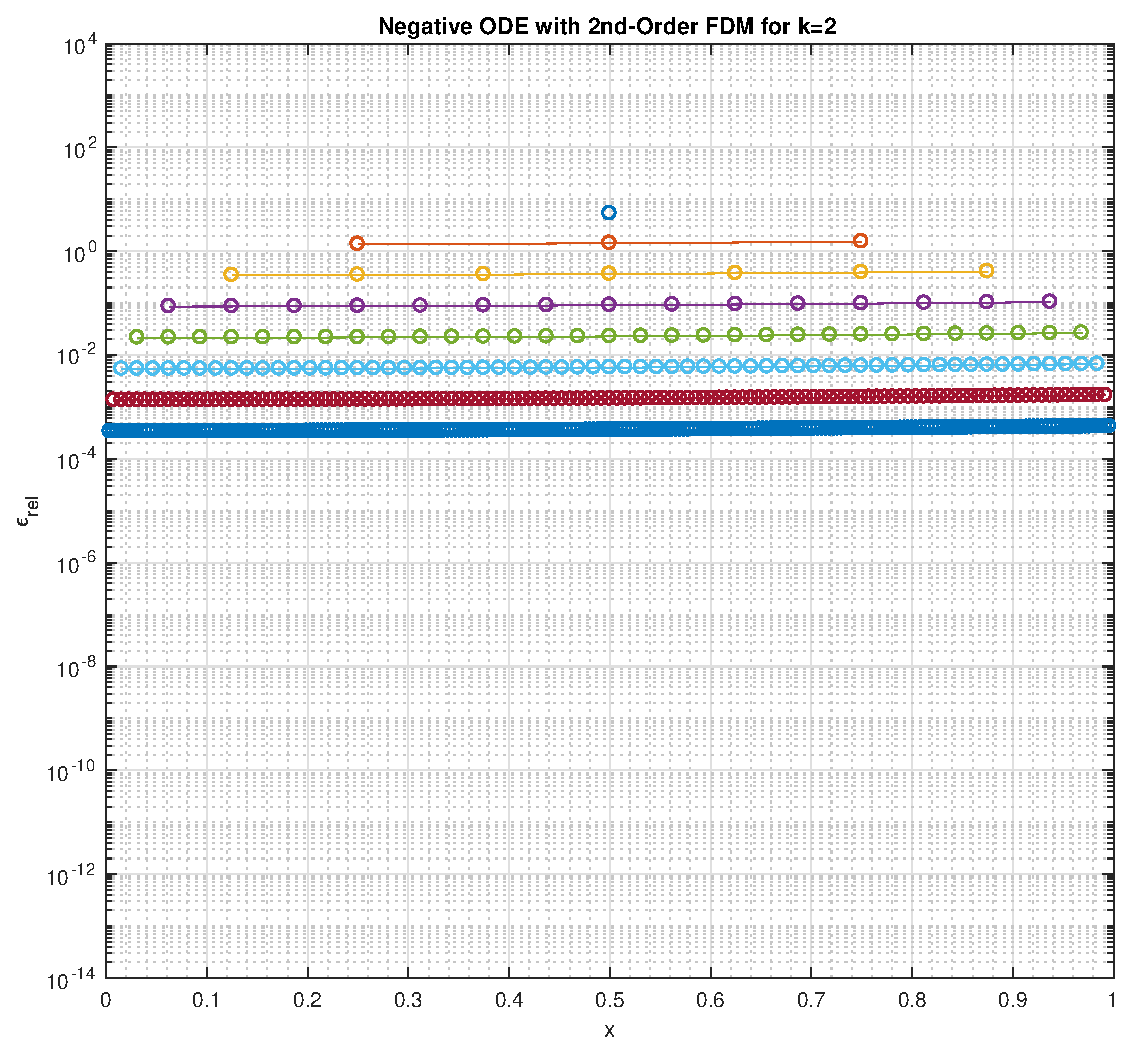
\includegraphics[width = 0.31\linewidth]{error_negative_ode_order_2_k_2}
		\caption{2nd-Order CDS FDM and Pointwise Error for Diffusion Equation with $k = 2$}
	\end{center}
\end{figure}

\begin{figure}[H]
	\begin{center}
		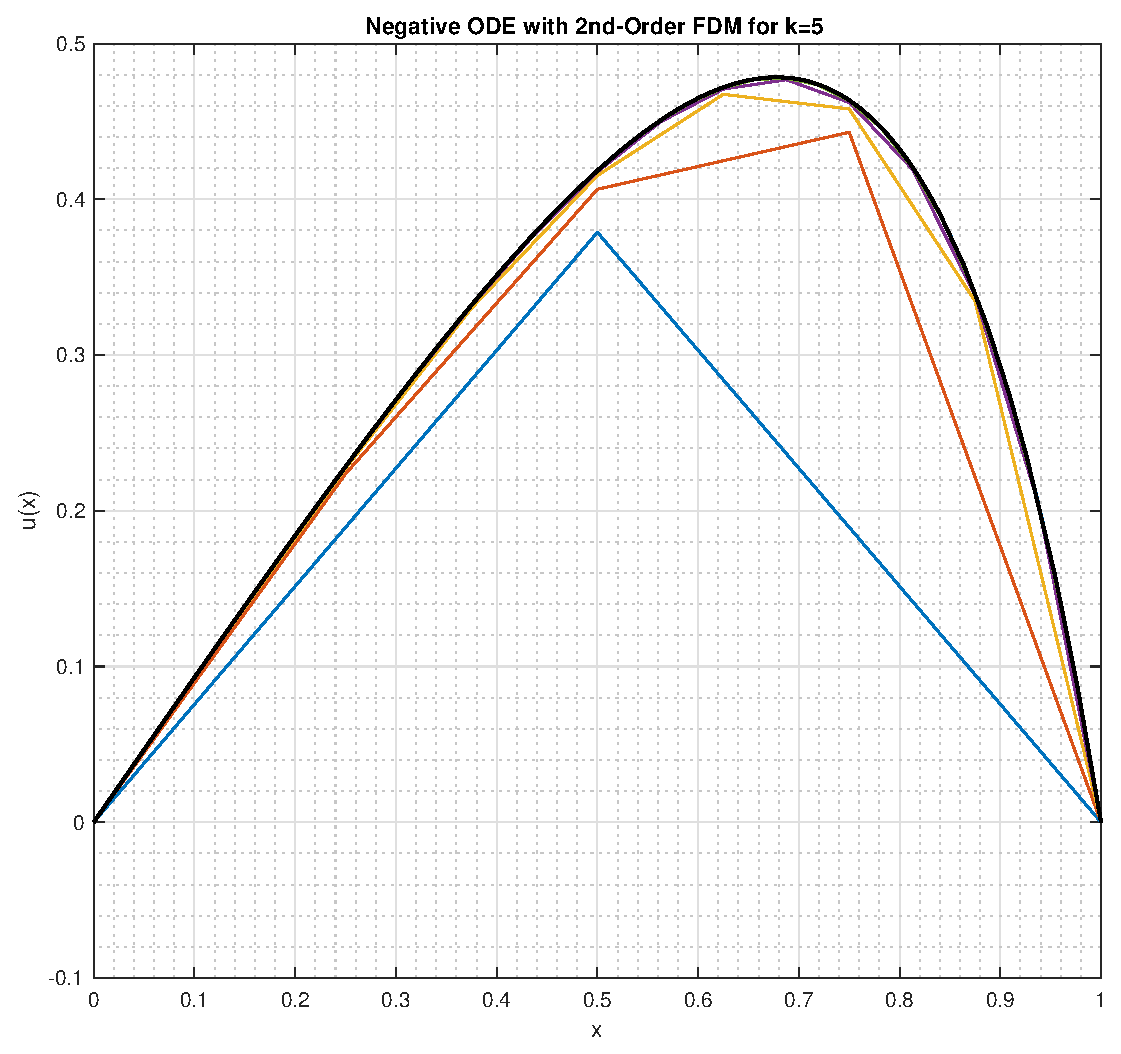
\includegraphics[width = 0.31\linewidth]{negative_ode_order_2_k_5}
		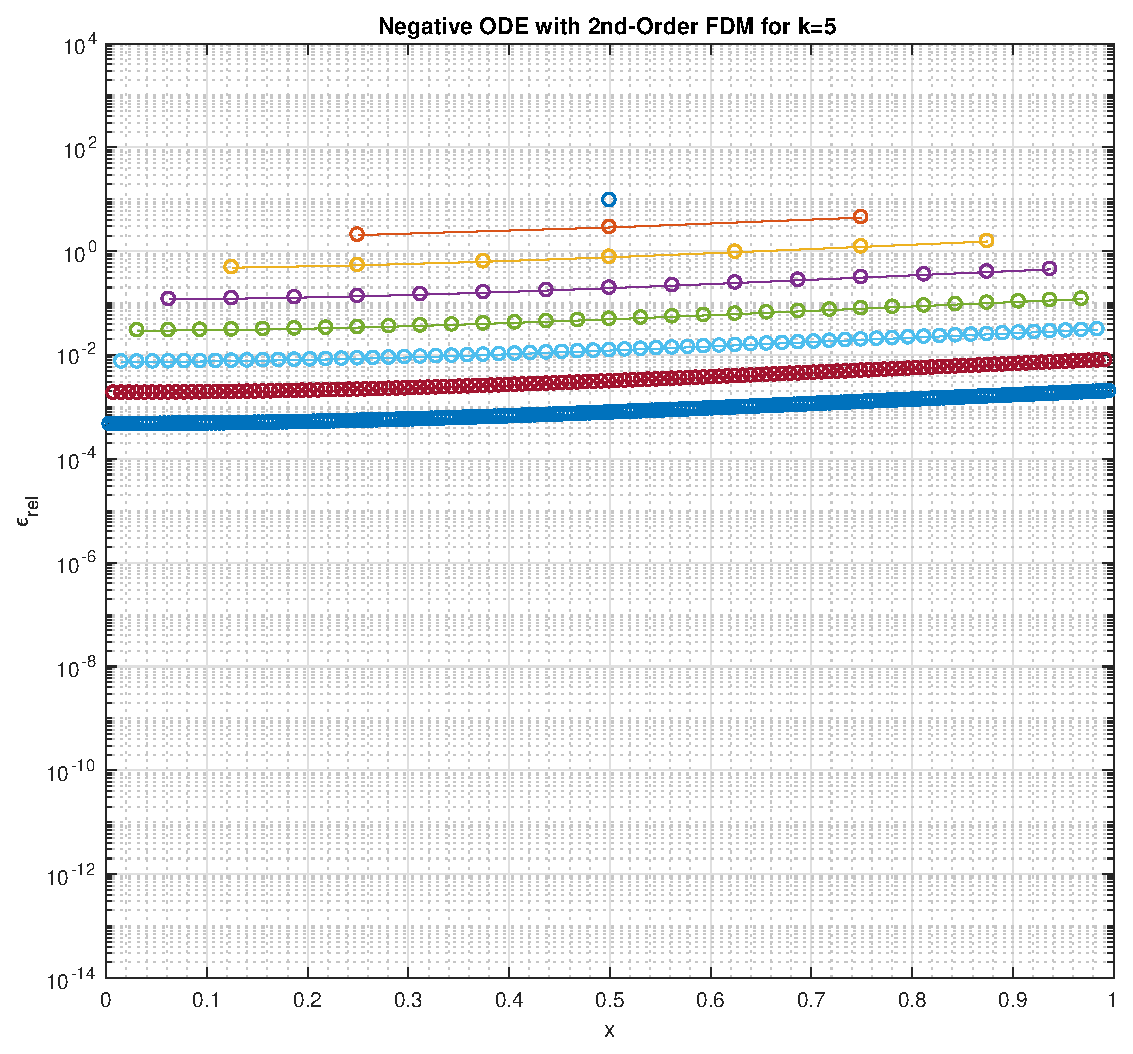
\includegraphics[width = 0.31\linewidth]{error_negative_ode_order_2_k_5}
		\caption{2nd-Order CDS FDM and Pointwise Error for Diffusion Equation with $k = 5$}
	\end{center}
\end{figure}

\newpage

\begin{figure}[H]
	\begin{center}
		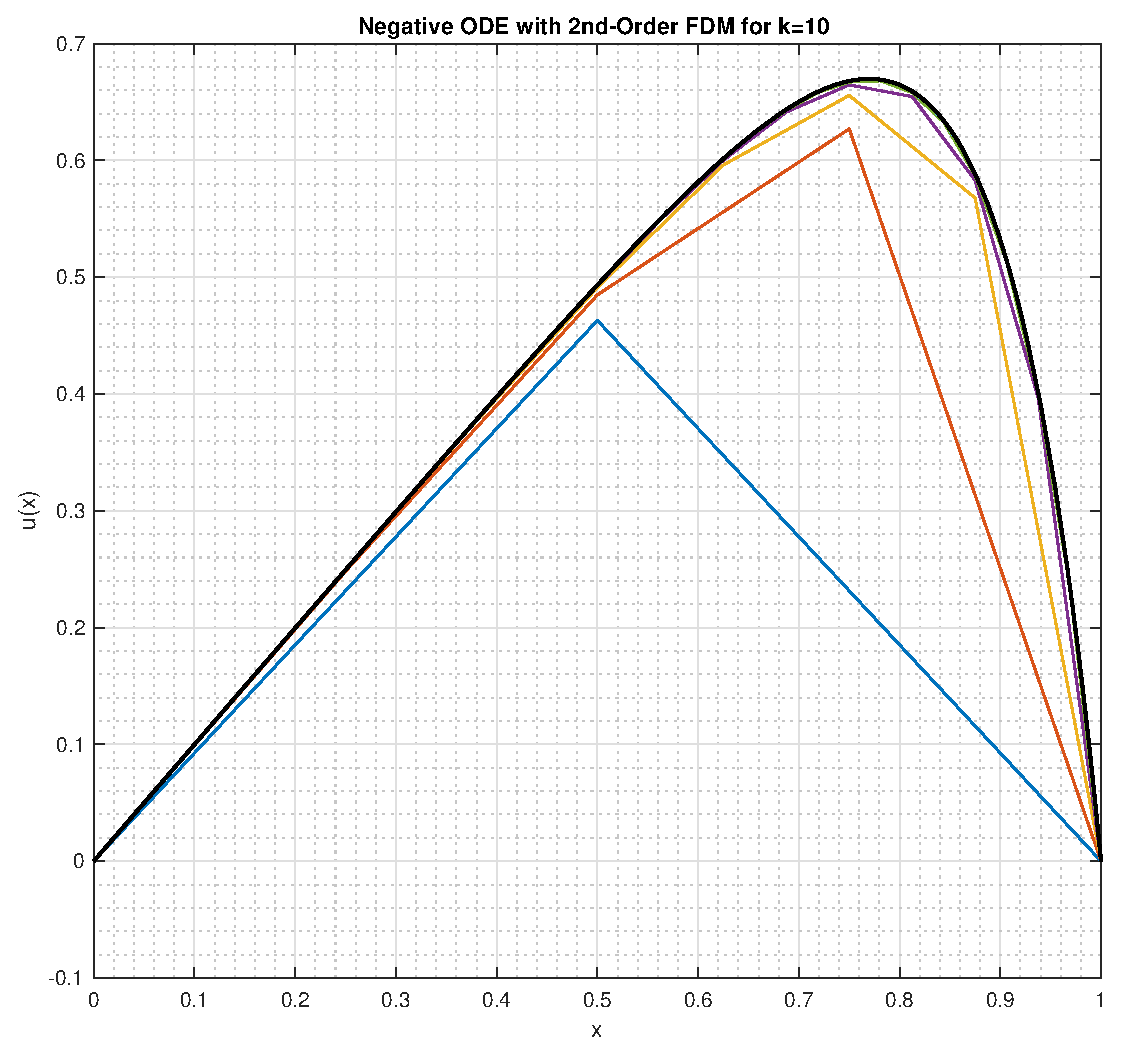
\includegraphics[width = 0.31\linewidth]{negative_ode_order_2_k_10}
		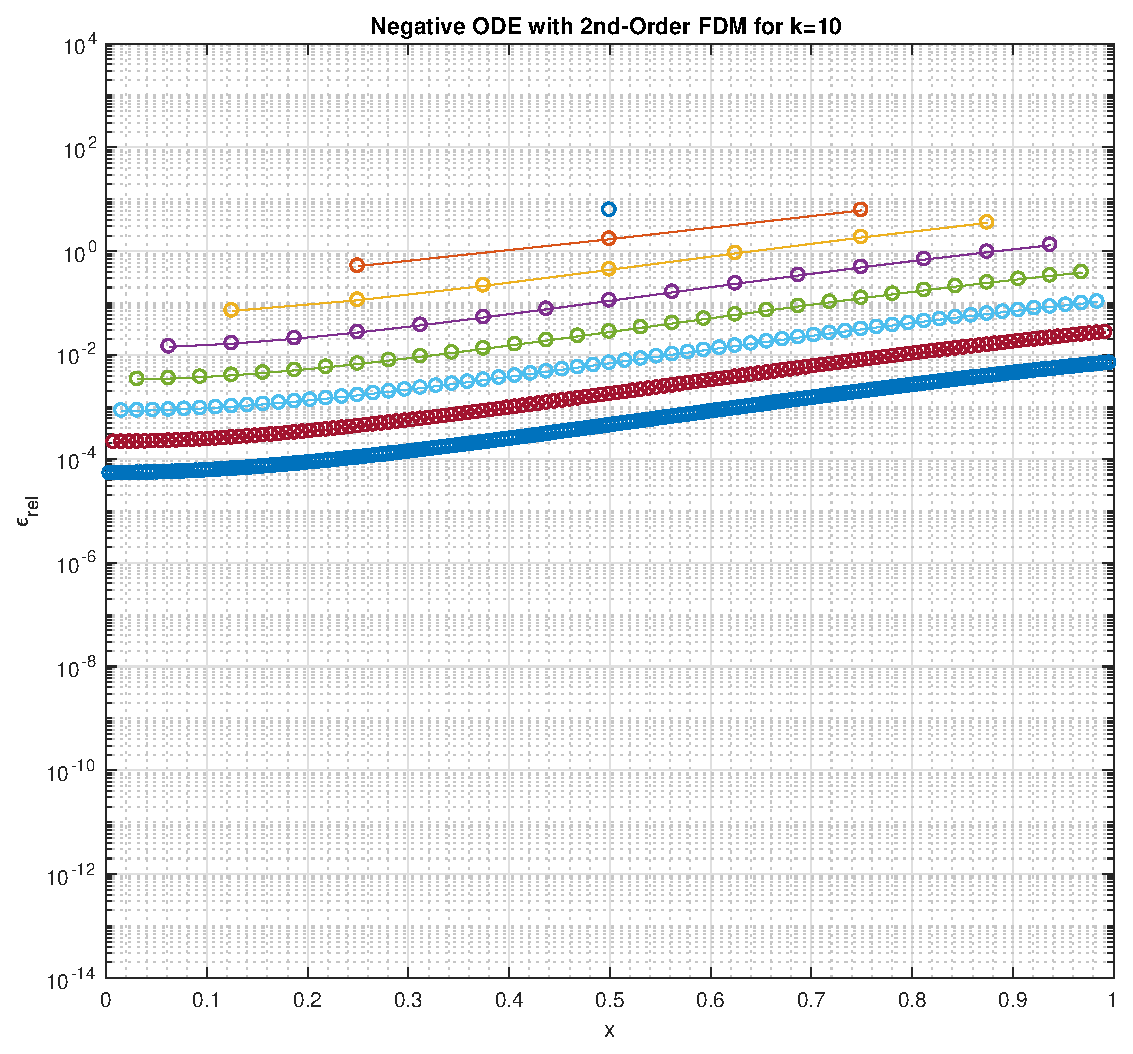
\includegraphics[width = 0.31\linewidth]{error_negative_ode_order_2_k_10}
		\caption{2nd-Order CDS FDM and Pointwise Error for Diffusion Equation with $k = 10$}
	\end{center}
\end{figure}

\begin{figure}[H]
	\begin{center}
		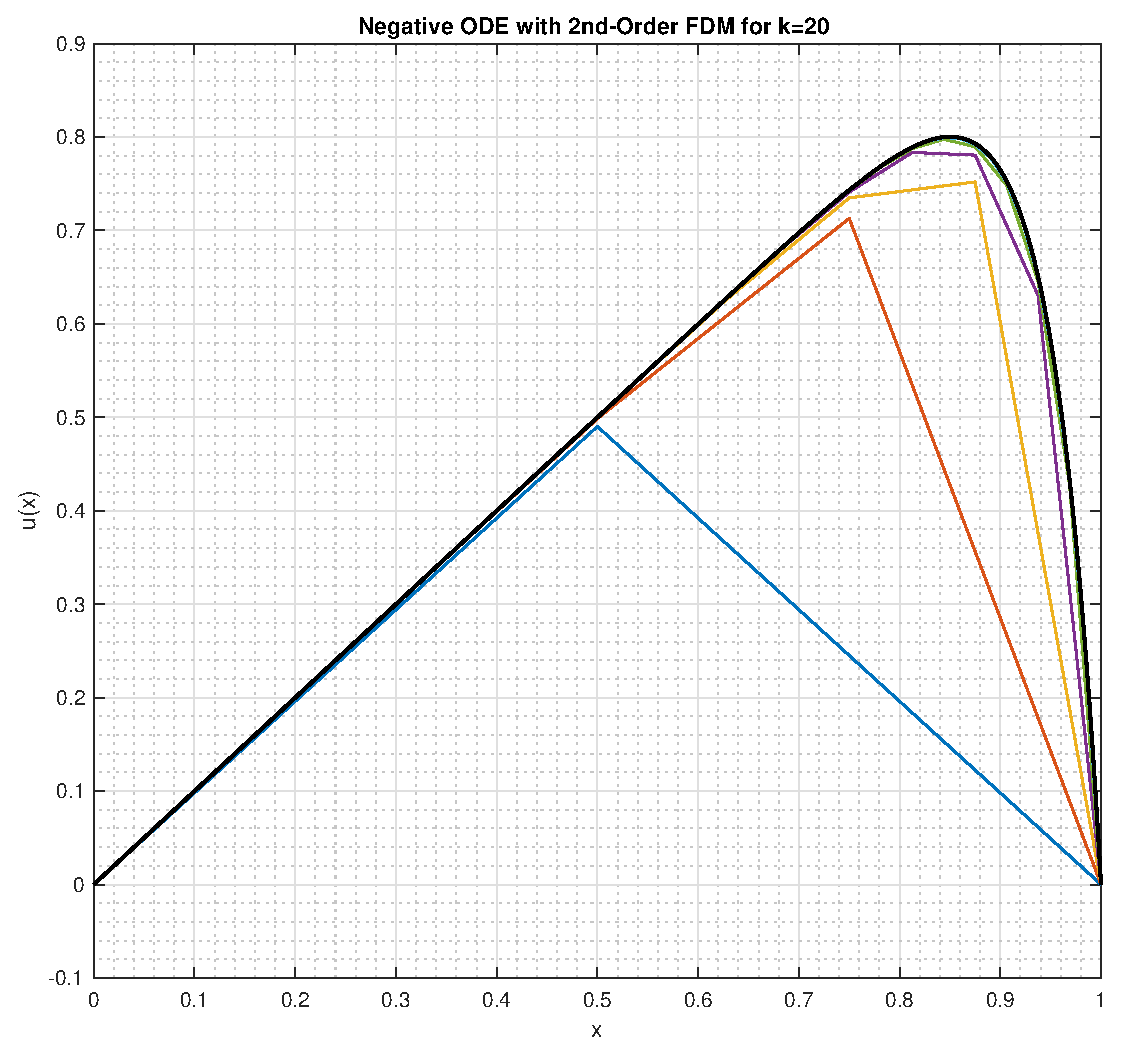
\includegraphics[width = 0.31\linewidth]{negative_ode_order_2_k_20}
		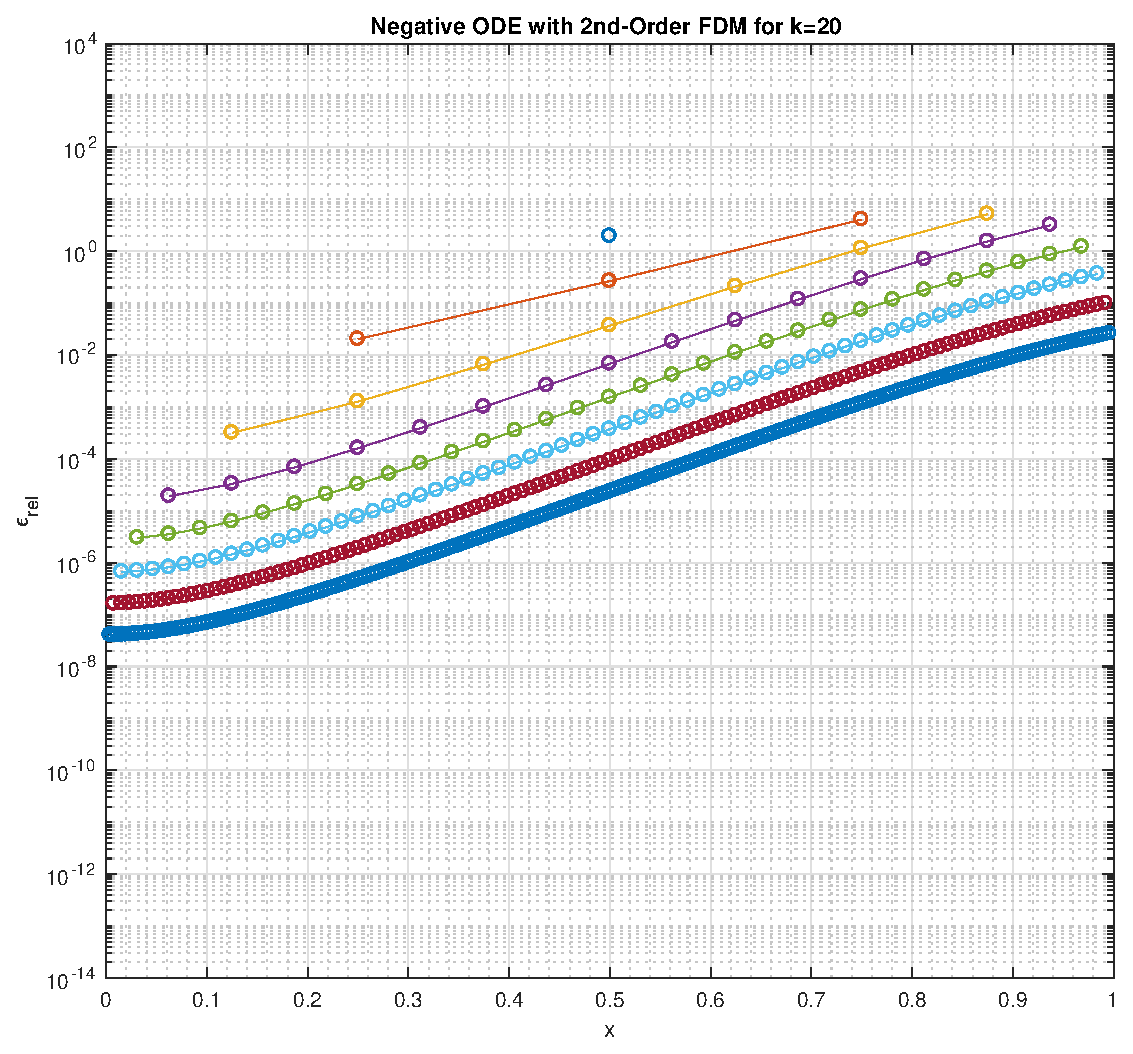
\includegraphics[width = 0.31\linewidth]{error_negative_ode_order_2_k_20}
		\caption{2nd-Order CDS FDM and Pointwise Error for Diffusion Equation with $k = 20$}
	\end{center}
\end{figure}

\begin{figure}[H]
	\begin{center}
		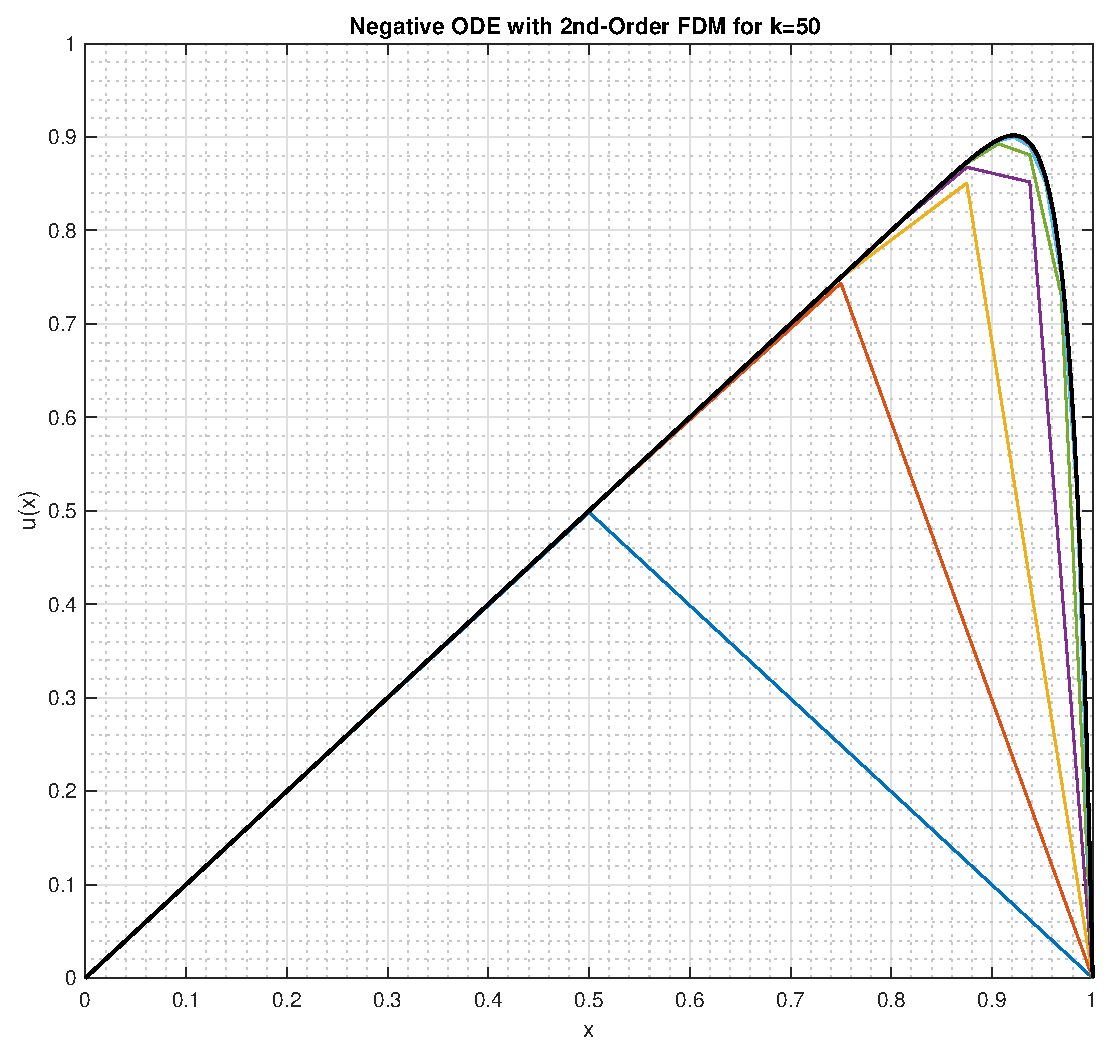
\includegraphics[width = 0.31\linewidth]{negative_ode_order_2_k_50}
		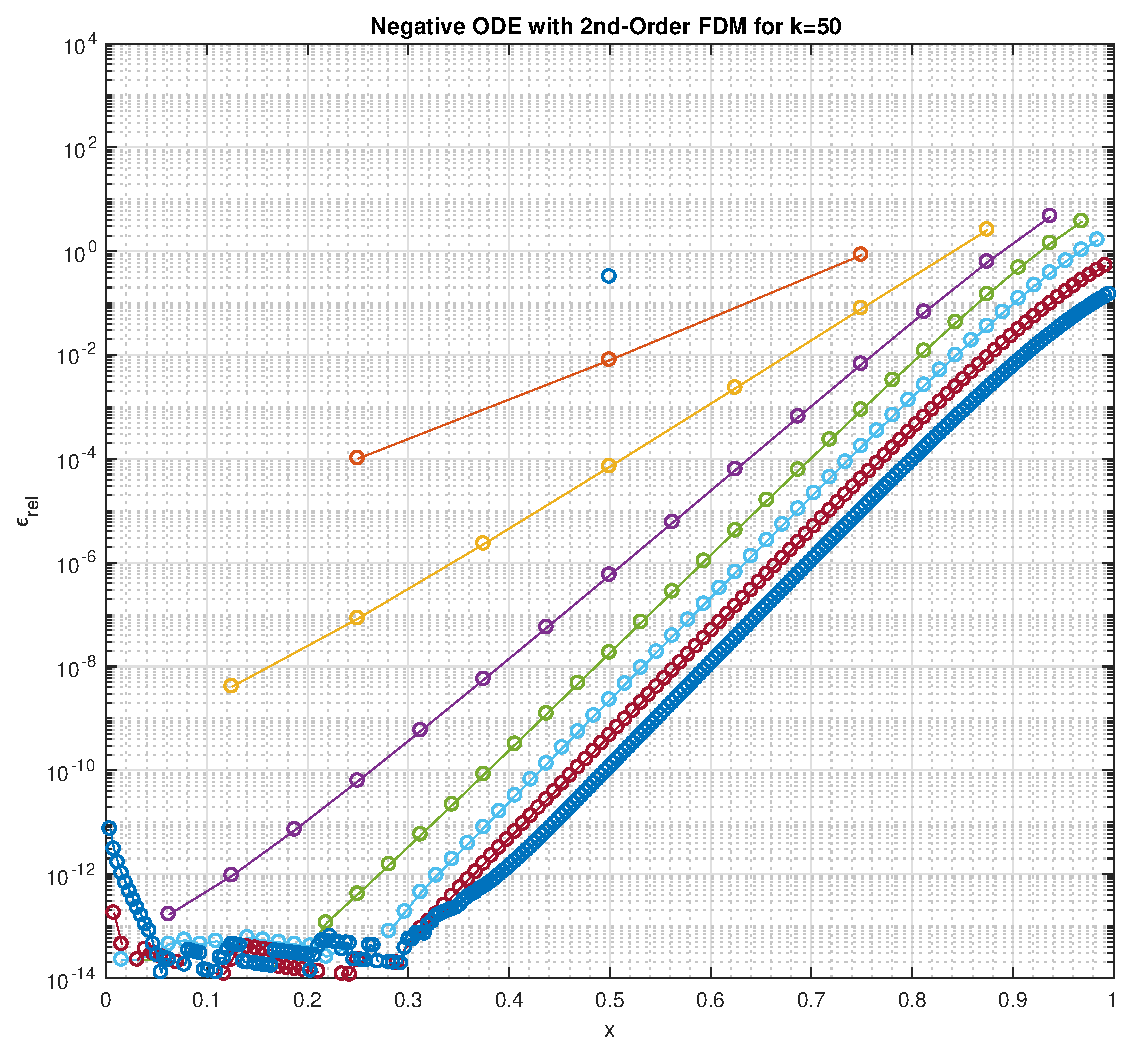
\includegraphics[width = 0.31\linewidth]{error_negative_ode_order_2_k_50}
		\caption{2nd-Order CDS FDM and Pointwise Error for Diffusion Equation with $k = 50$}
	\end{center}
\end{figure}

\begin{center}
	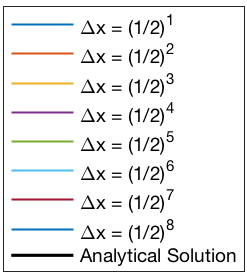
\includegraphics[height = 0.19\linewidth]{legend}
\end{center}

\newpage

\subsubsection{2nd-Order Central Difference Scheme - Harmonic Wave Equation}

\begin{figure}[H]
	\begin{center}
		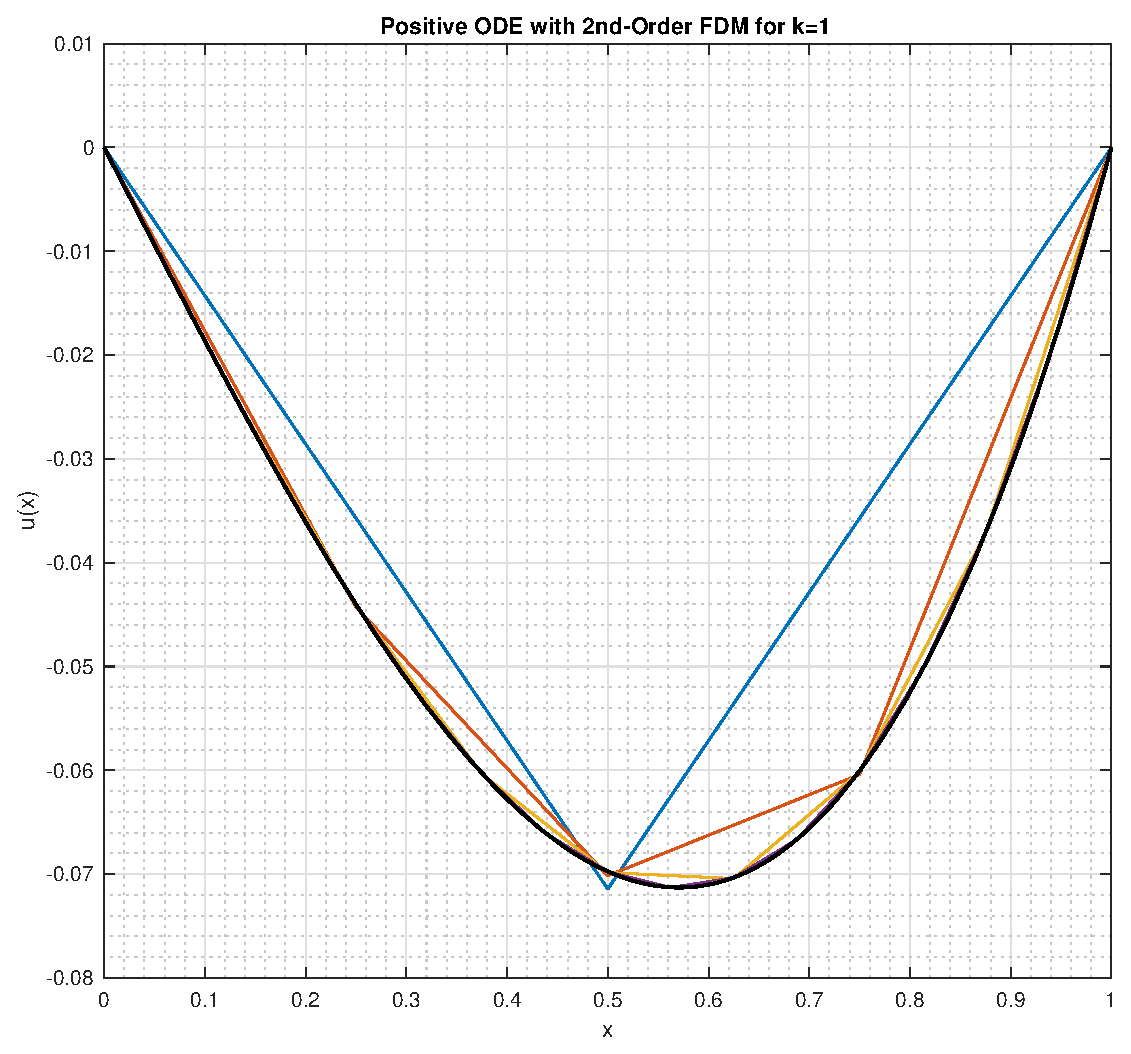
\includegraphics[width = 0.31\linewidth]{positive_ode_order_2_k_1}
		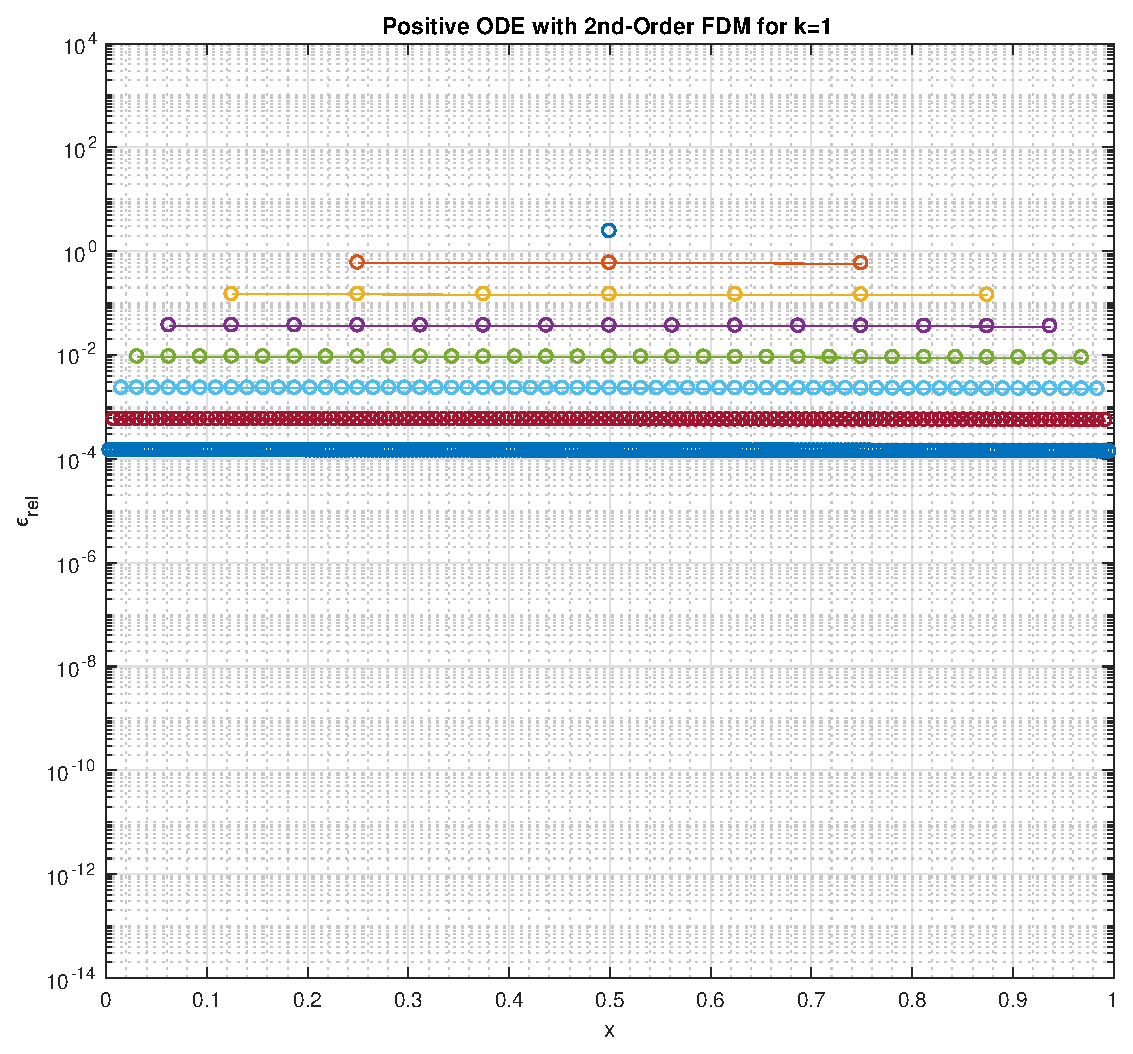
\includegraphics[width = 0.31\linewidth]{error_positive_ode_order_2_k_1}
		\caption{2nd-Order CDS FDM and Pointwise Error for Harmonic Wave Equation with $k = 1$}
	\end{center}
\end{figure}

\begin{figure}[H]
	\begin{center}
		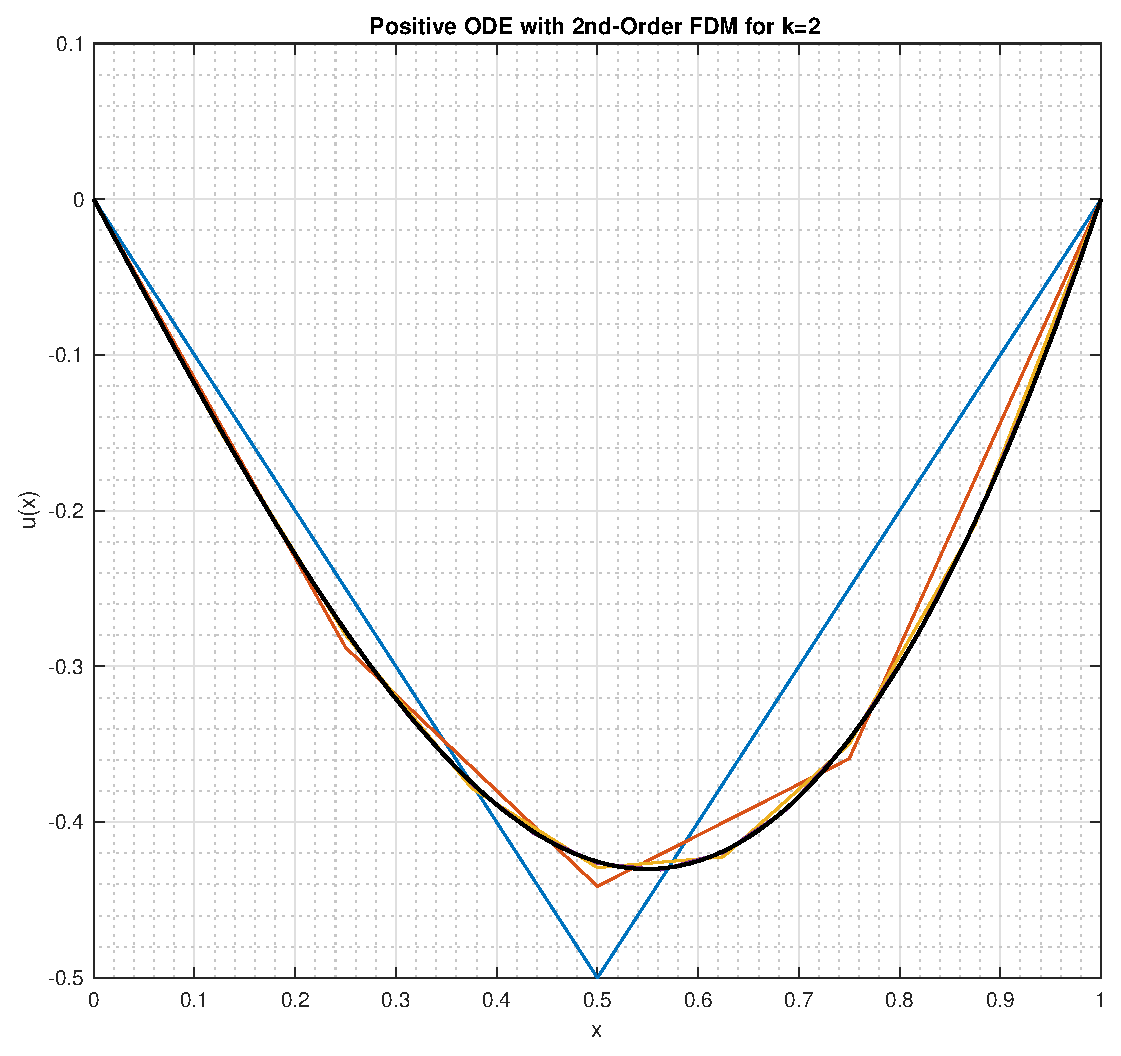
\includegraphics[width = 0.31\linewidth]{positive_ode_order_2_k_2}
		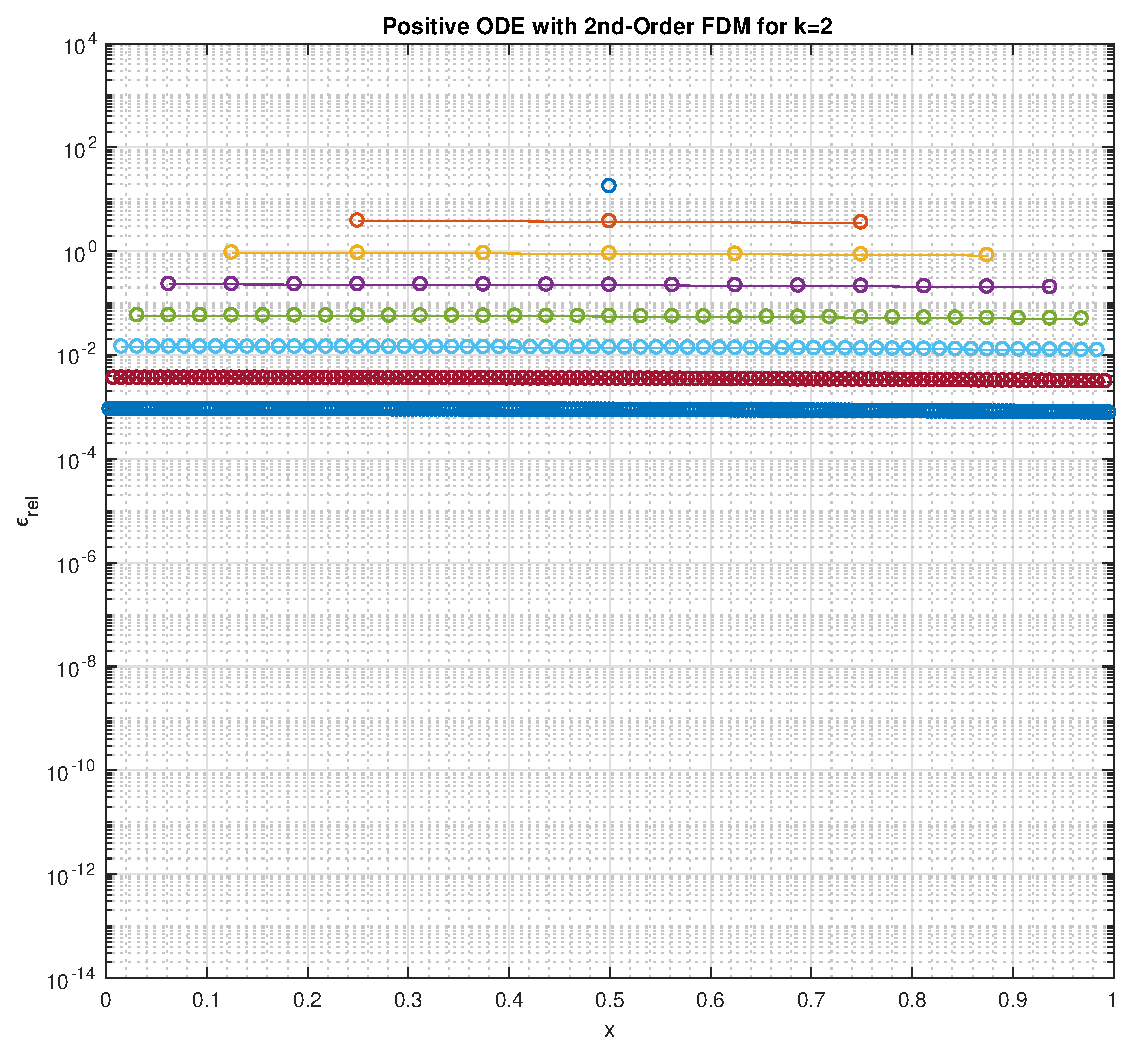
\includegraphics[width = 0.31\linewidth]{error_positive_ode_order_2_k_2}
		\caption{2nd-Order CDS FDM and Pointwise Error for Harmonic Wave Equation with $k = 2$}
	\end{center}
\end{figure}

\begin{figure}[H]
	\begin{center}
		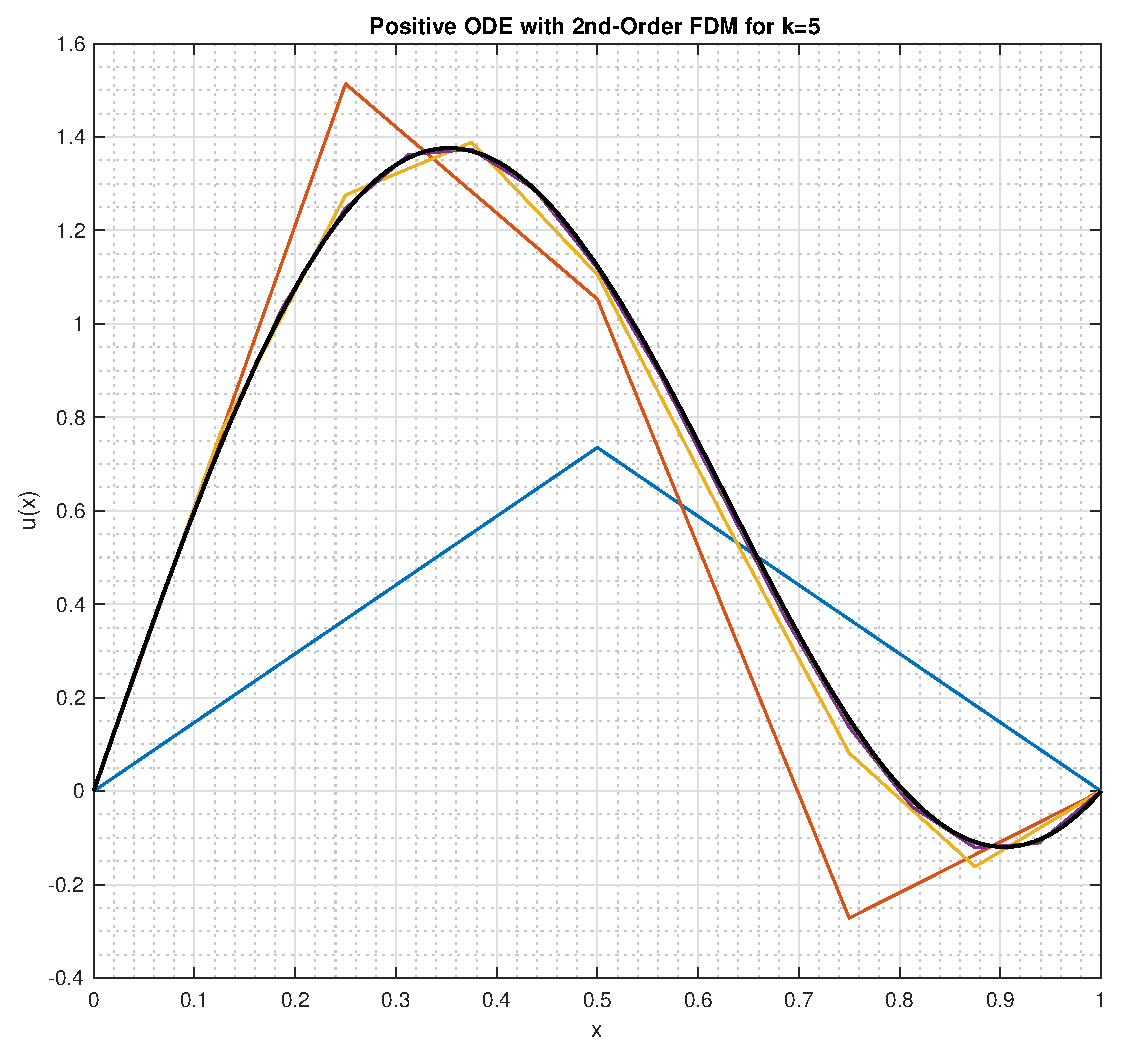
\includegraphics[width = 0.31\linewidth]{positive_ode_order_2_k_5}
		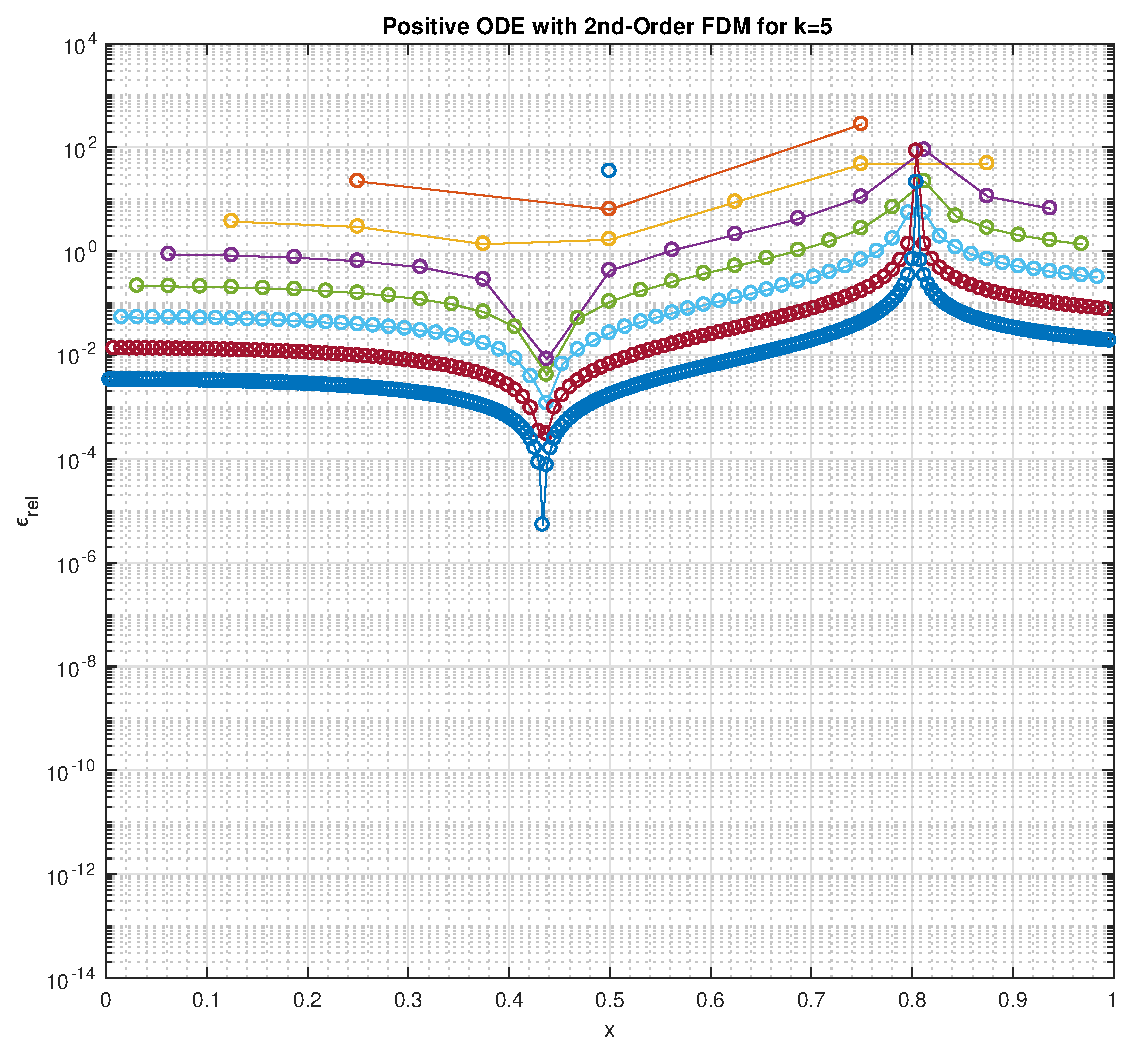
\includegraphics[width = 0.31\linewidth]{error_positive_ode_order_2_k_5}
		\caption{2nd-Order CDS FDM and Pointwise Error for Harmonic Wave Equation with $k = 5$}
	\end{center}
\end{figure}

\newpage

\begin{figure}[H]
	\begin{center}
		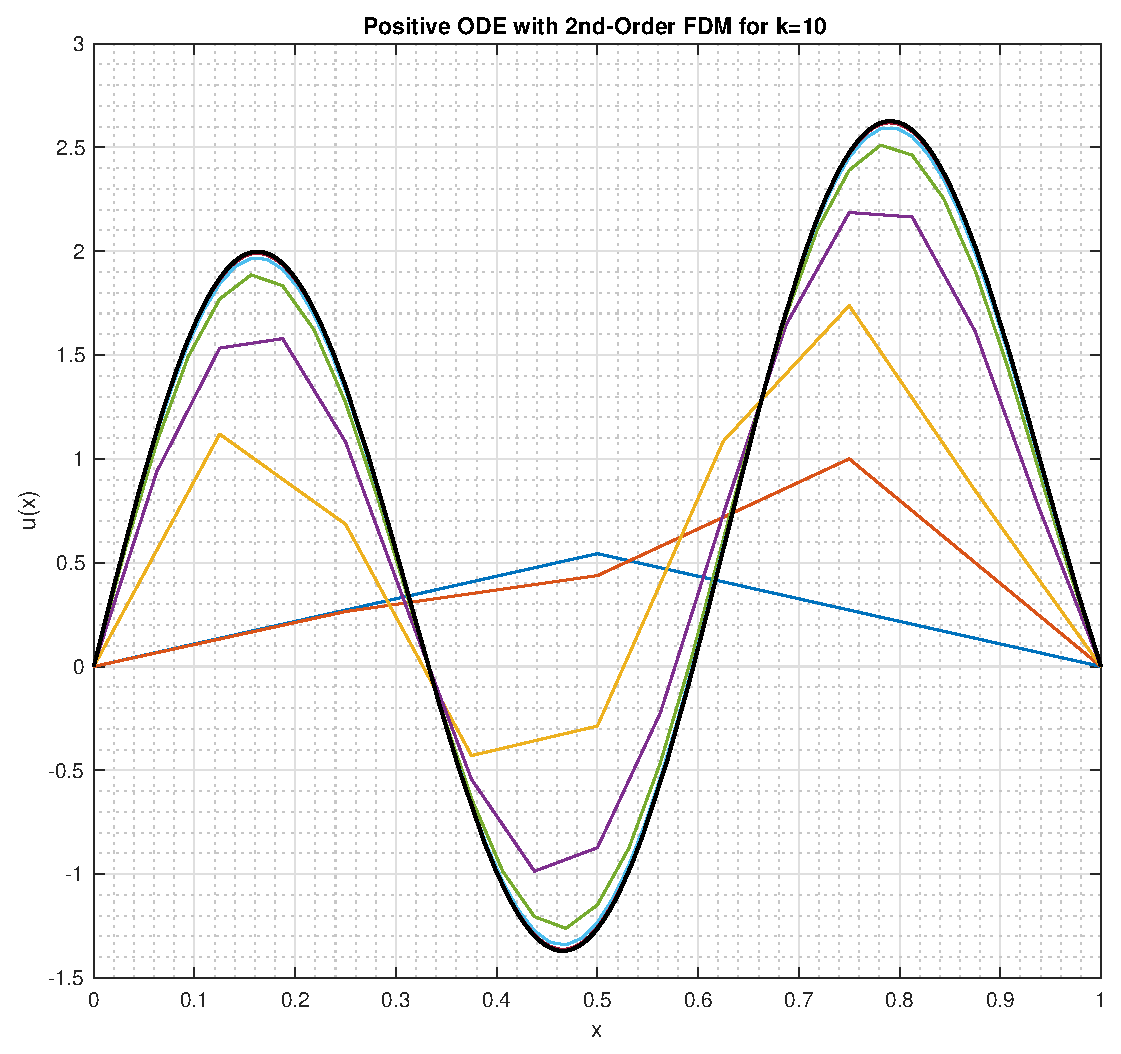
\includegraphics[width = 0.31\linewidth]{positive_ode_order_2_k_10}
		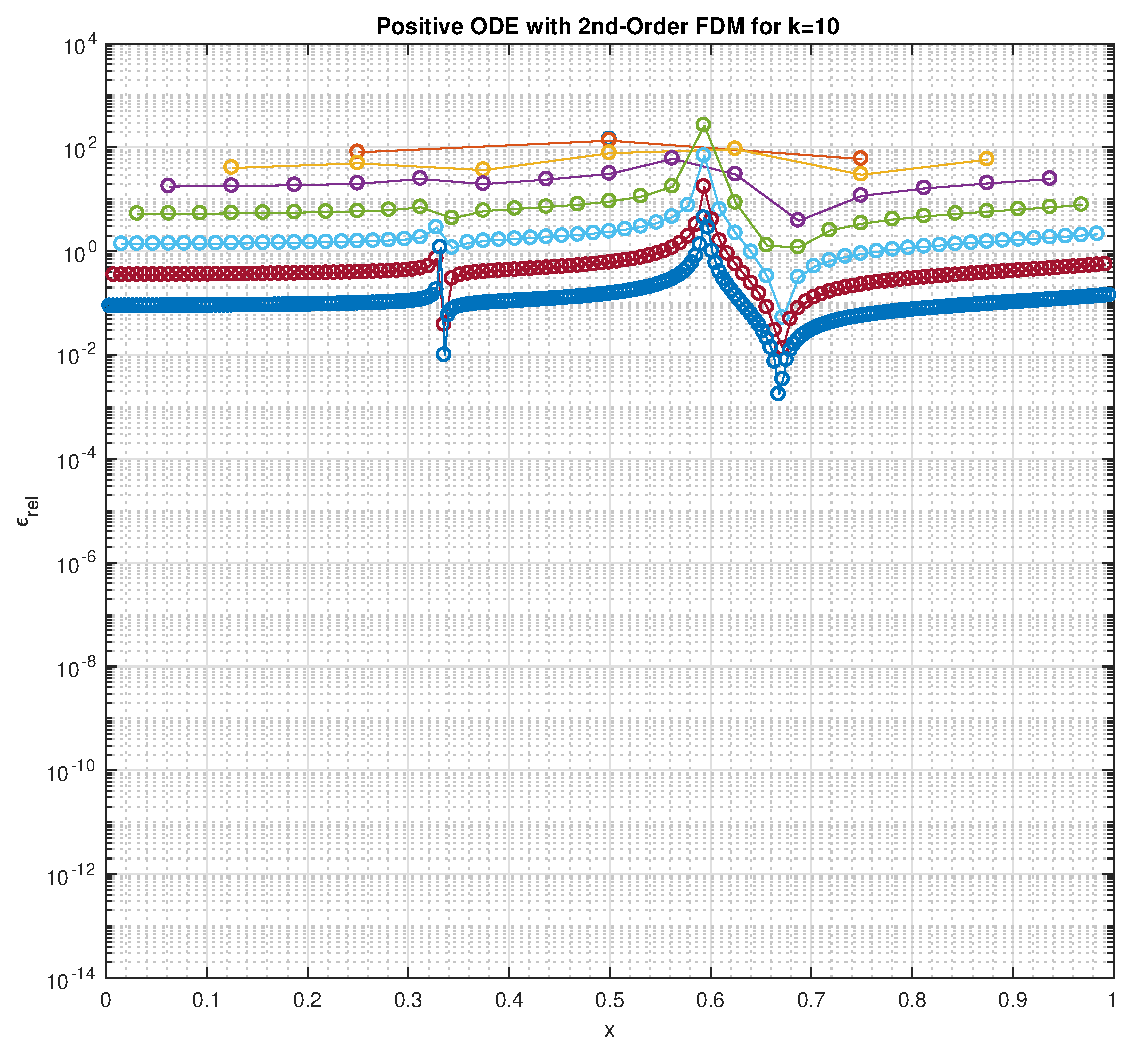
\includegraphics[width = 0.31\linewidth]{error_positive_ode_order_2_k_10}
		\caption{2nd-Order CDS FDM and Pointwise Error for Harmonic Wave Equation with $k = 10$}
	\end{center}
\end{figure}

\begin{figure}[H]
	\begin{center}
		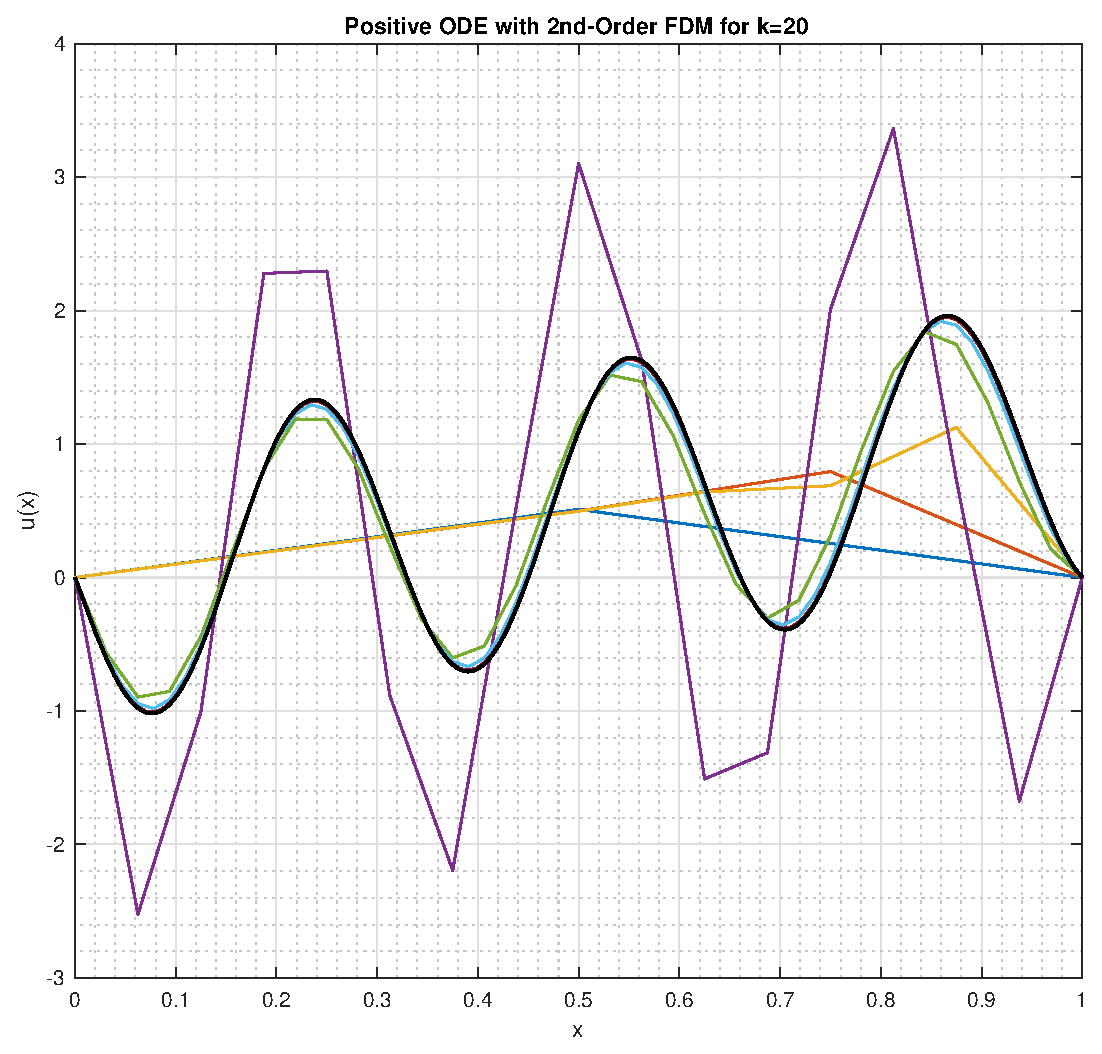
\includegraphics[width = 0.31\linewidth]{positive_ode_order_2_k_20}
		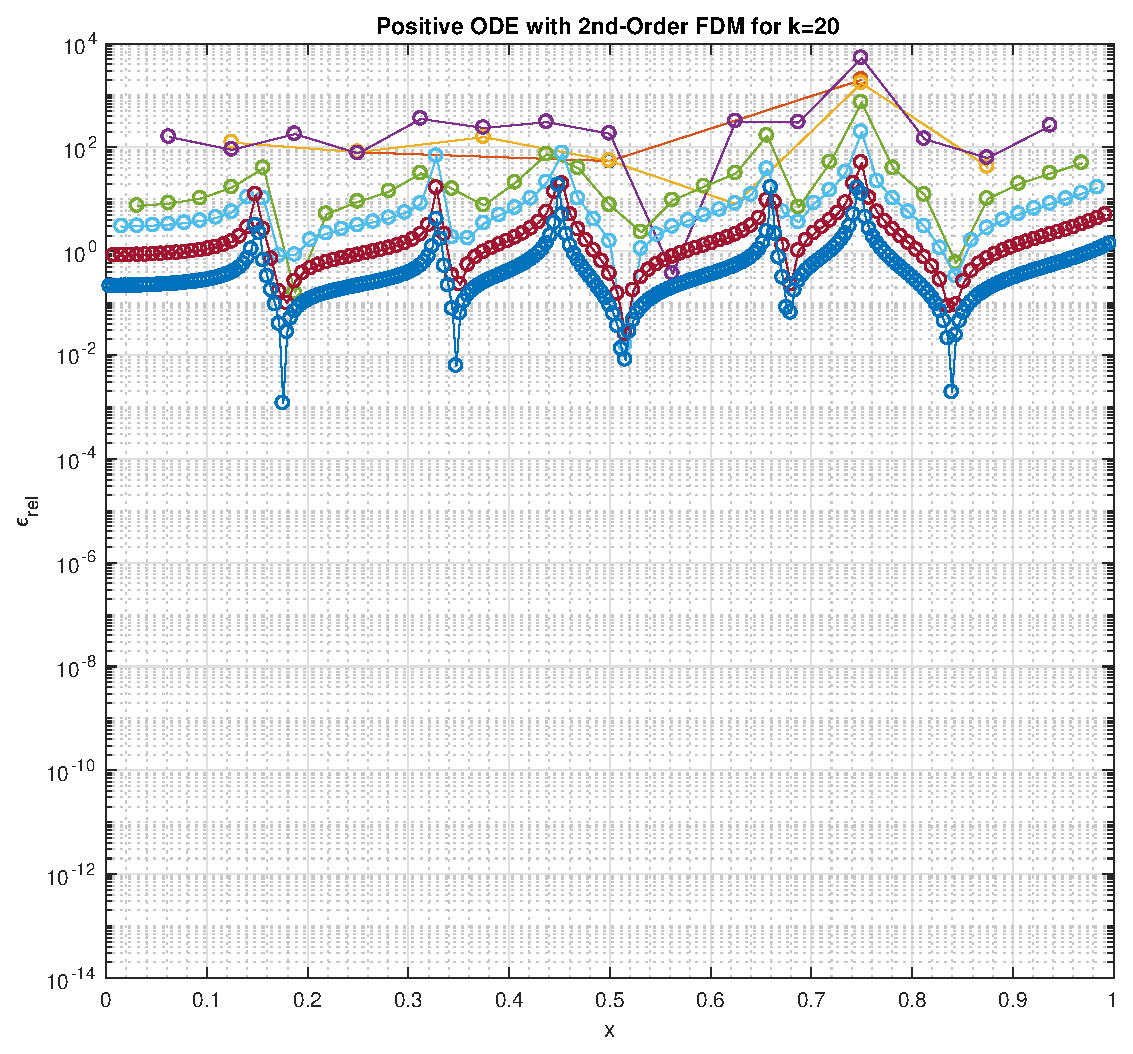
\includegraphics[width = 0.31\linewidth]{error_positive_ode_order_2_k_20}
		\caption{2nd-Order CDS FDM and Pointwise Error for Harmonic Wave Equation with $k = 20$}
	\end{center}
\end{figure}

\begin{figure}[H]
	\begin{center}
		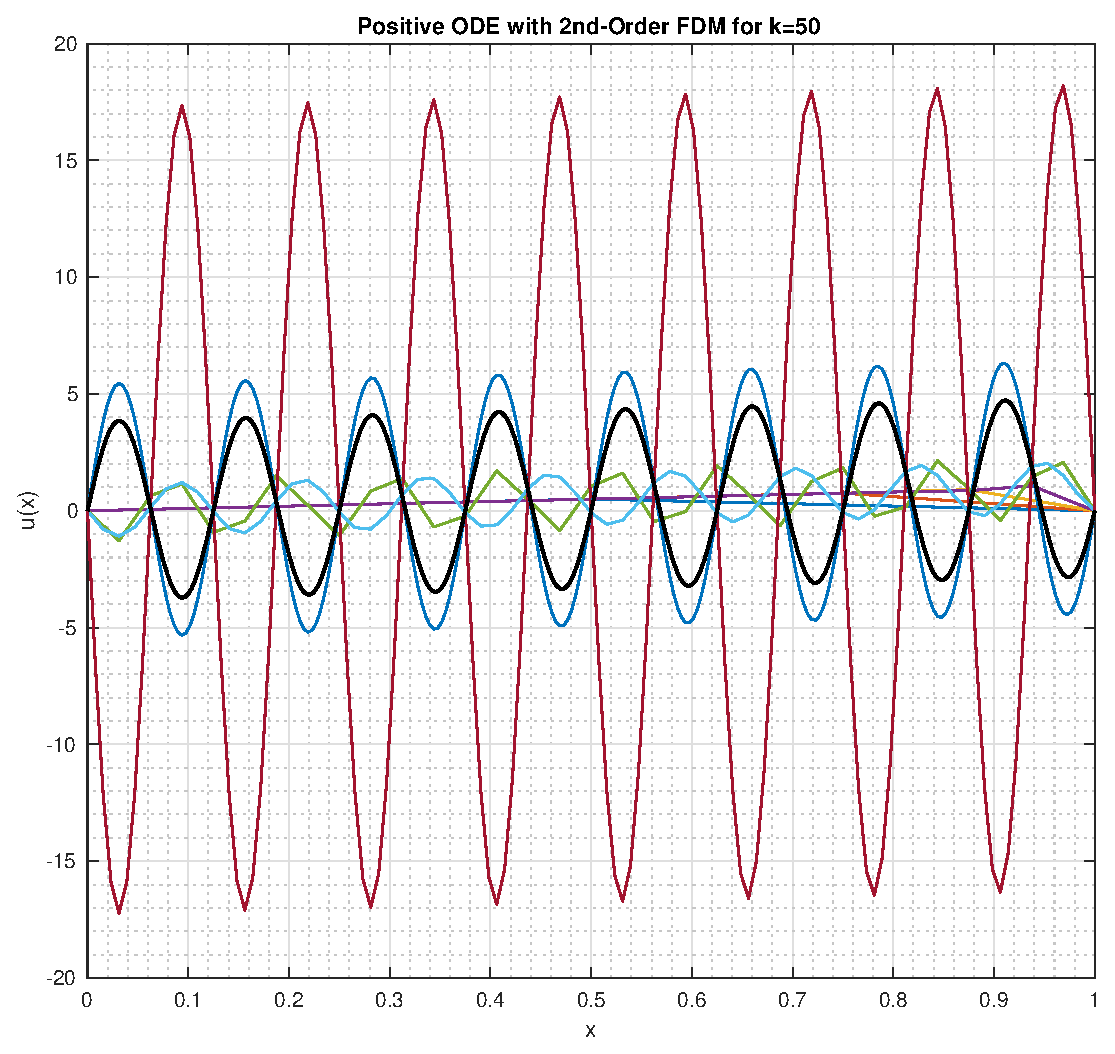
\includegraphics[width = 0.31\linewidth]{positive_ode_order_2_k_50}
		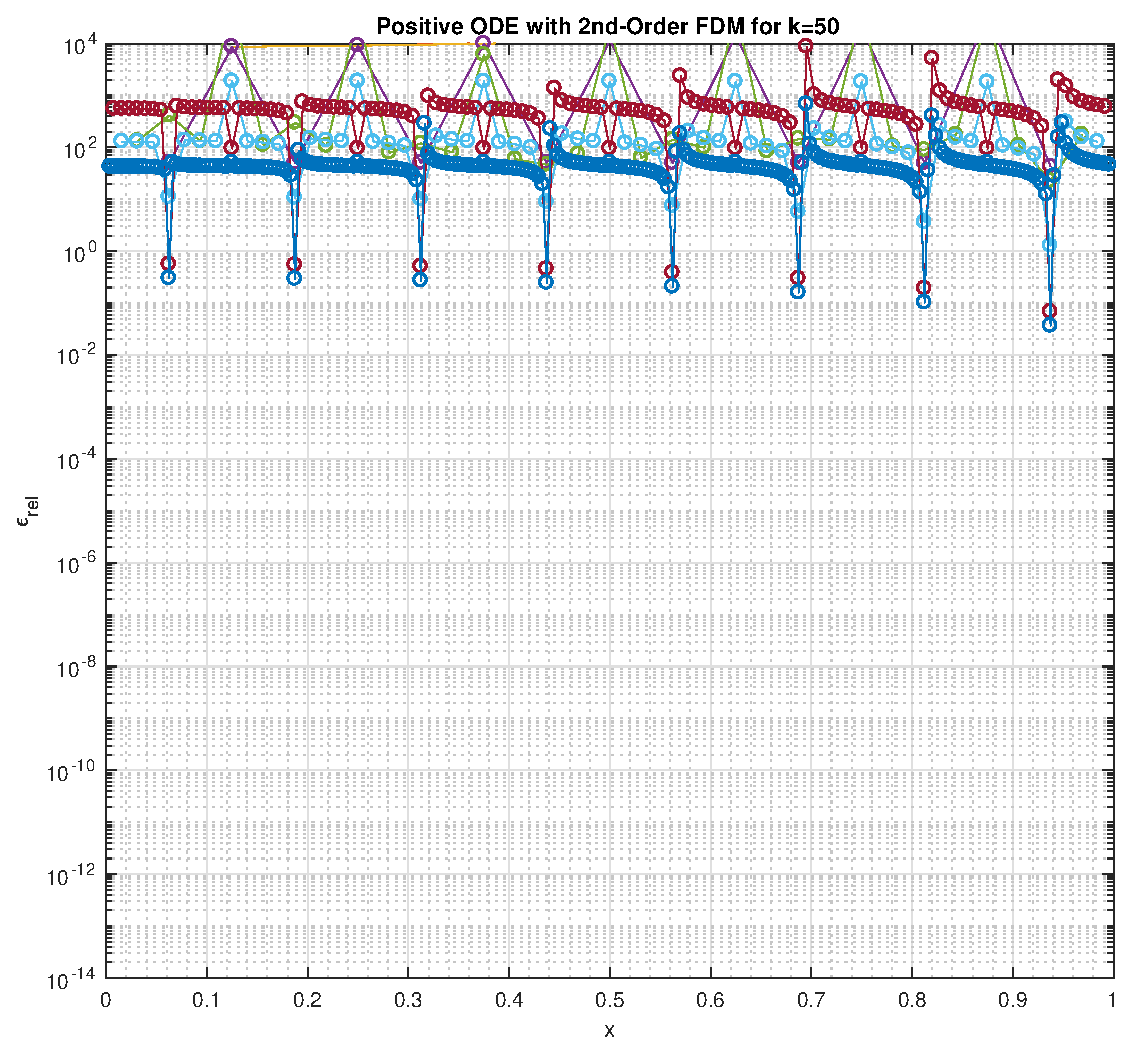
\includegraphics[width = 0.31\linewidth]{error_positive_ode_order_2_k_50}
		\caption{2nd-Order CDS FDM and Pointwise Error for Harmonic Wave Equation with $k = 50$}
	\end{center}
\end{figure}

\begin{center}
	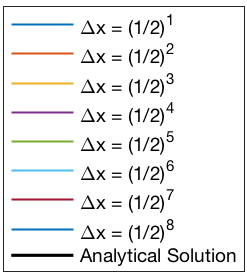
\includegraphics[height = 0.11\linewidth]{legend}
\end{center}

\newpage

\subsubsection{2nd-Order Central Difference Scheme - Convection-Diffusion Equation}

\begin{figure}[H]
	\begin{center}
		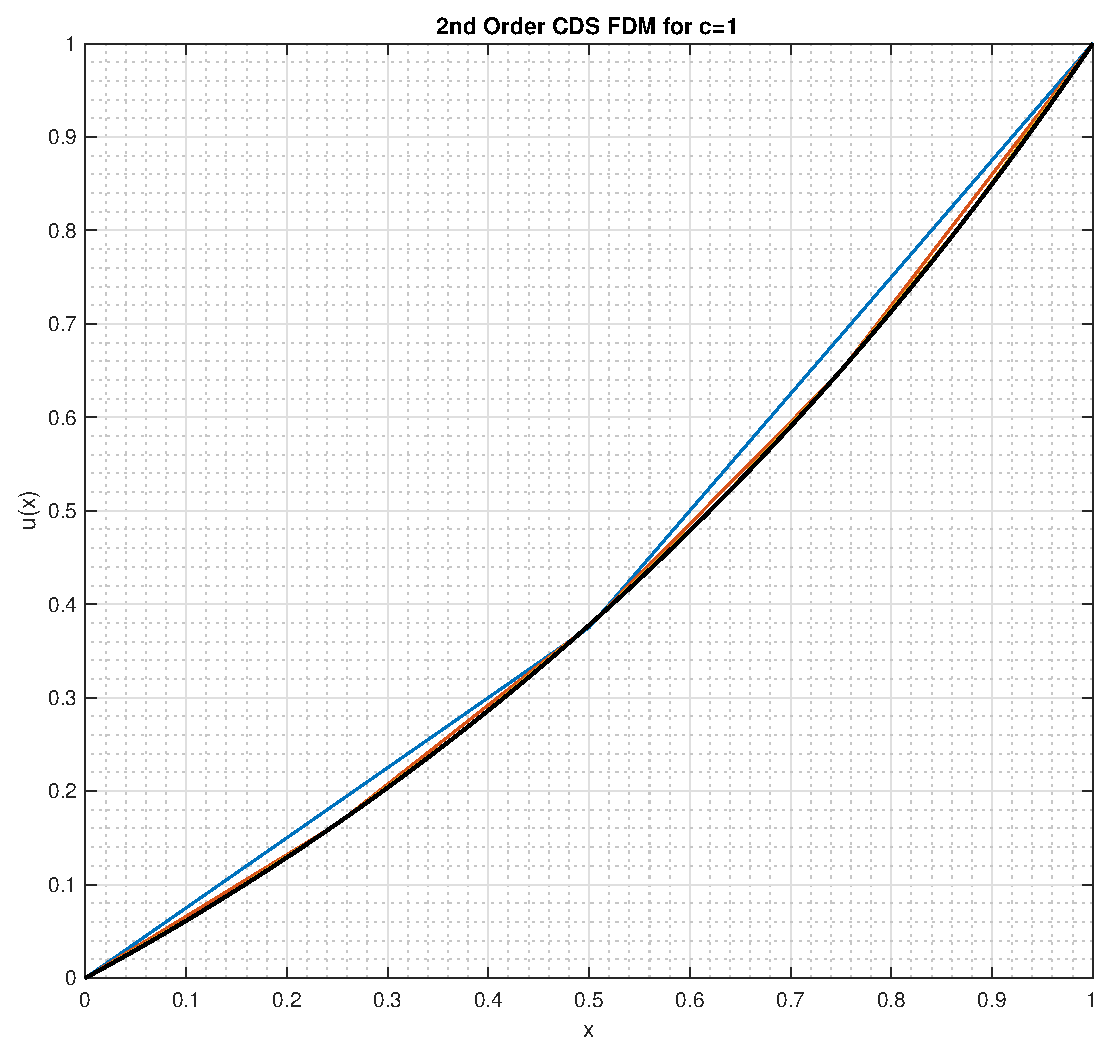
\includegraphics[width = 0.31\linewidth]{solution_2nd_order_cds_c_1}
		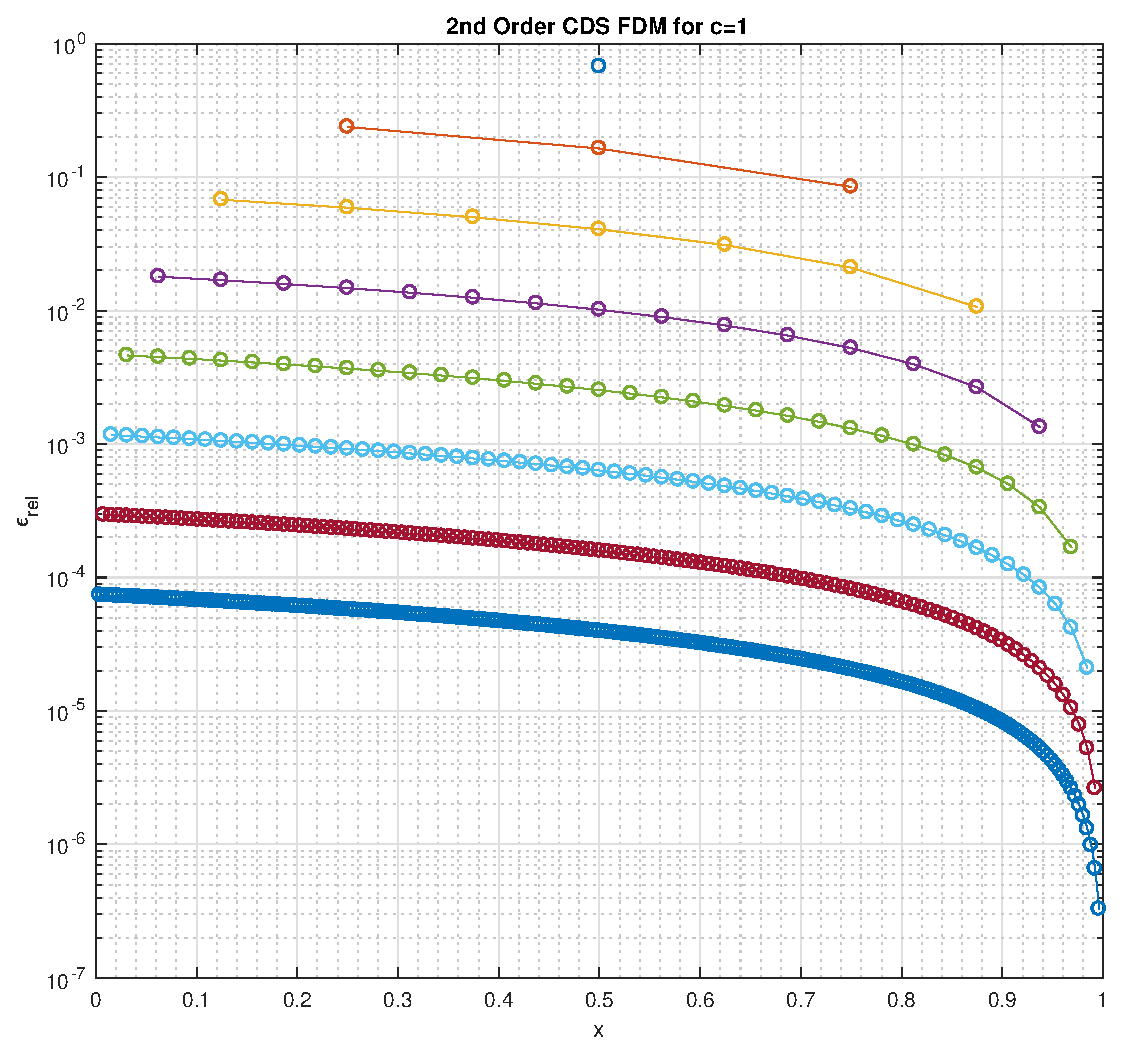
\includegraphics[width = 0.31\linewidth]{pointwise_error_2nd_order_cds_c_1}
		\caption{2nd-Order CDS FDM and Pointwise Error for Convection-Diffusion Equation with $c = 1$}
	\end{center}
\end{figure}

\begin{figure}[H]
	\begin{center}
		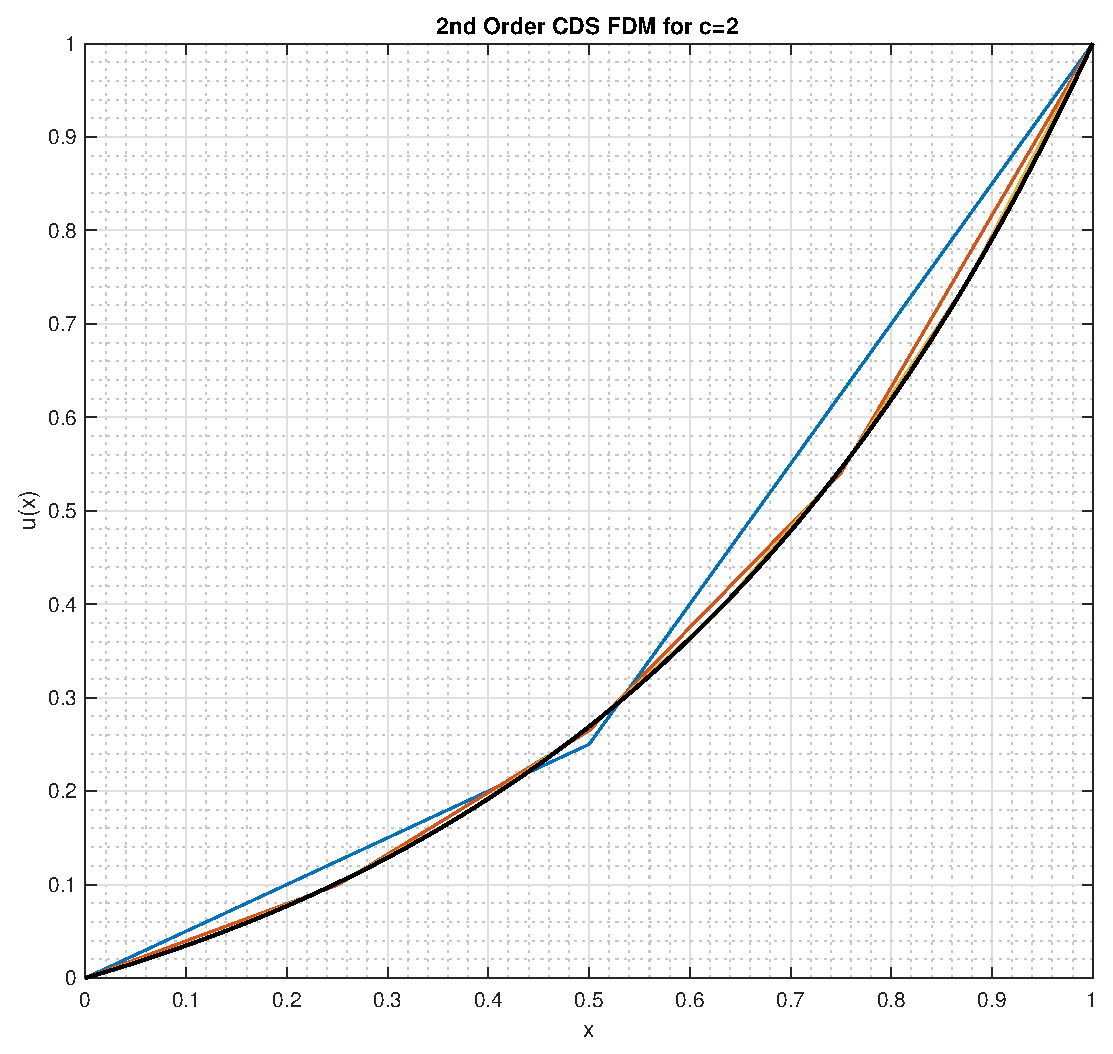
\includegraphics[width = 0.31\linewidth]{solution_2nd_order_cds_c_2}
		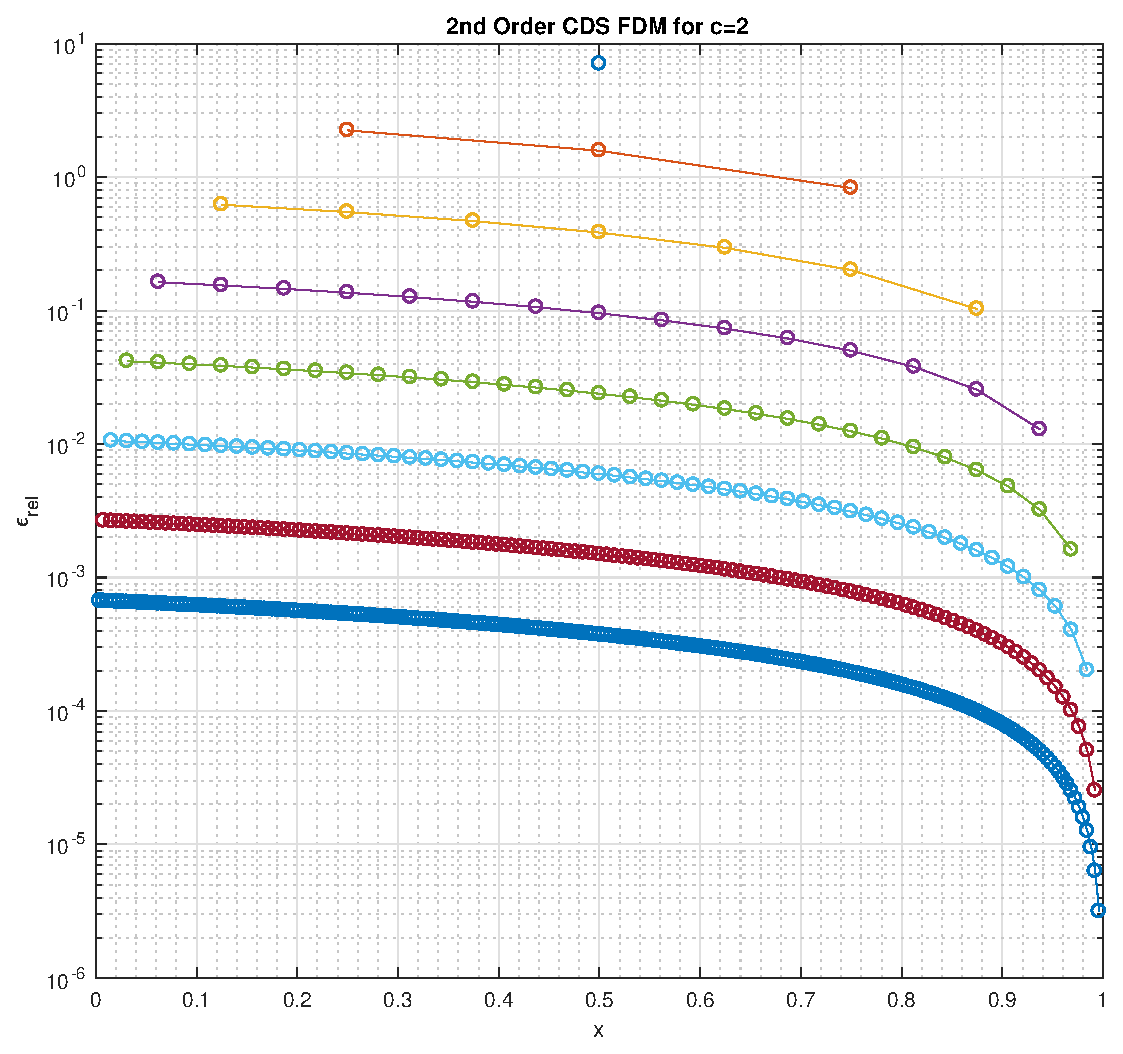
\includegraphics[width = 0.31\linewidth]{pointwise_error_2nd_order_cds_c_2}
		\caption{2nd-Order CDS FDM and Pointwise Error for Convection-Diffusion Equation with $c = 2$}
	\end{center}
\end{figure}

\begin{figure}[H]
	\begin{center}
		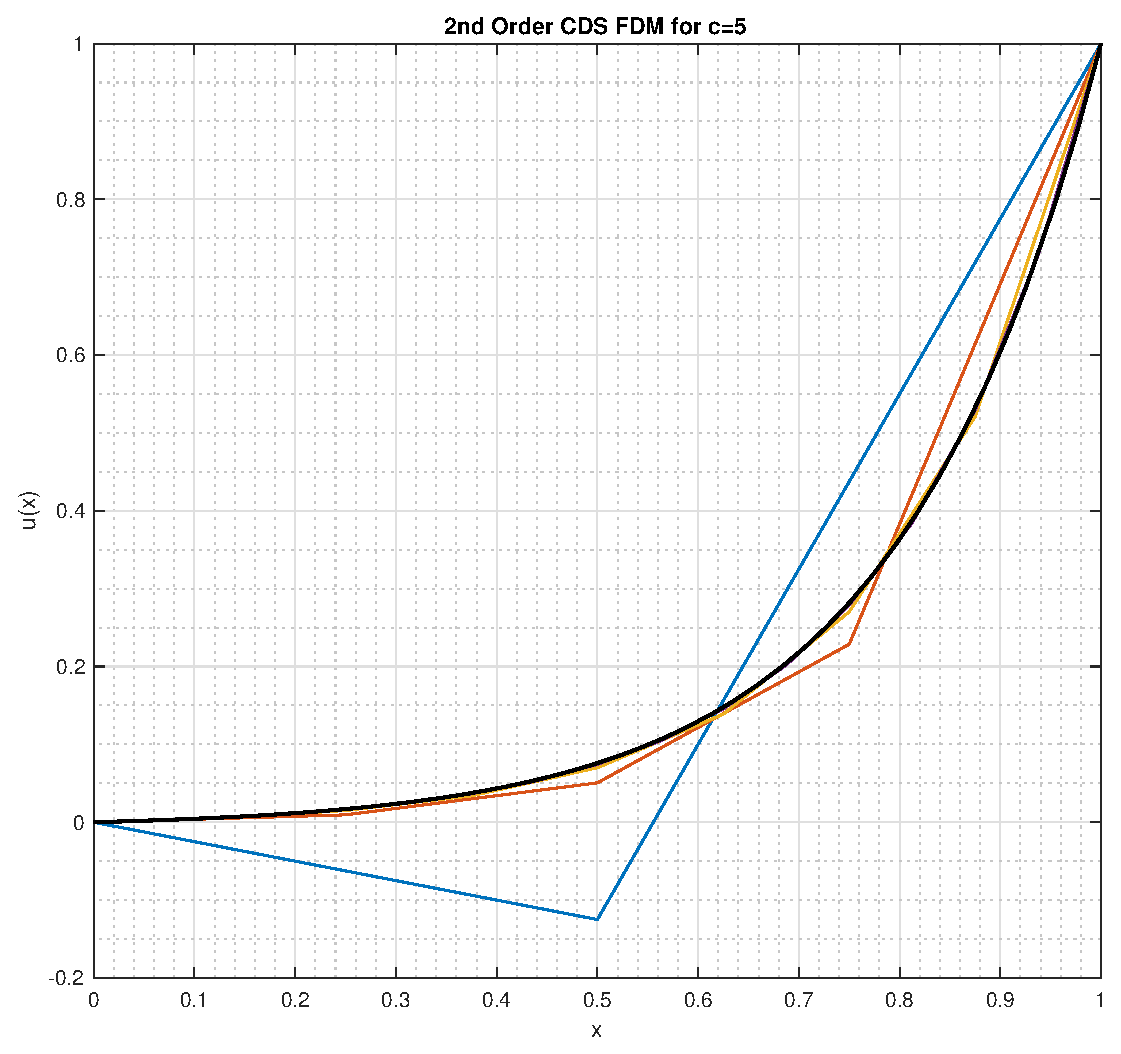
\includegraphics[width = 0.31\linewidth]{solution_2nd_order_cds_c_5}
		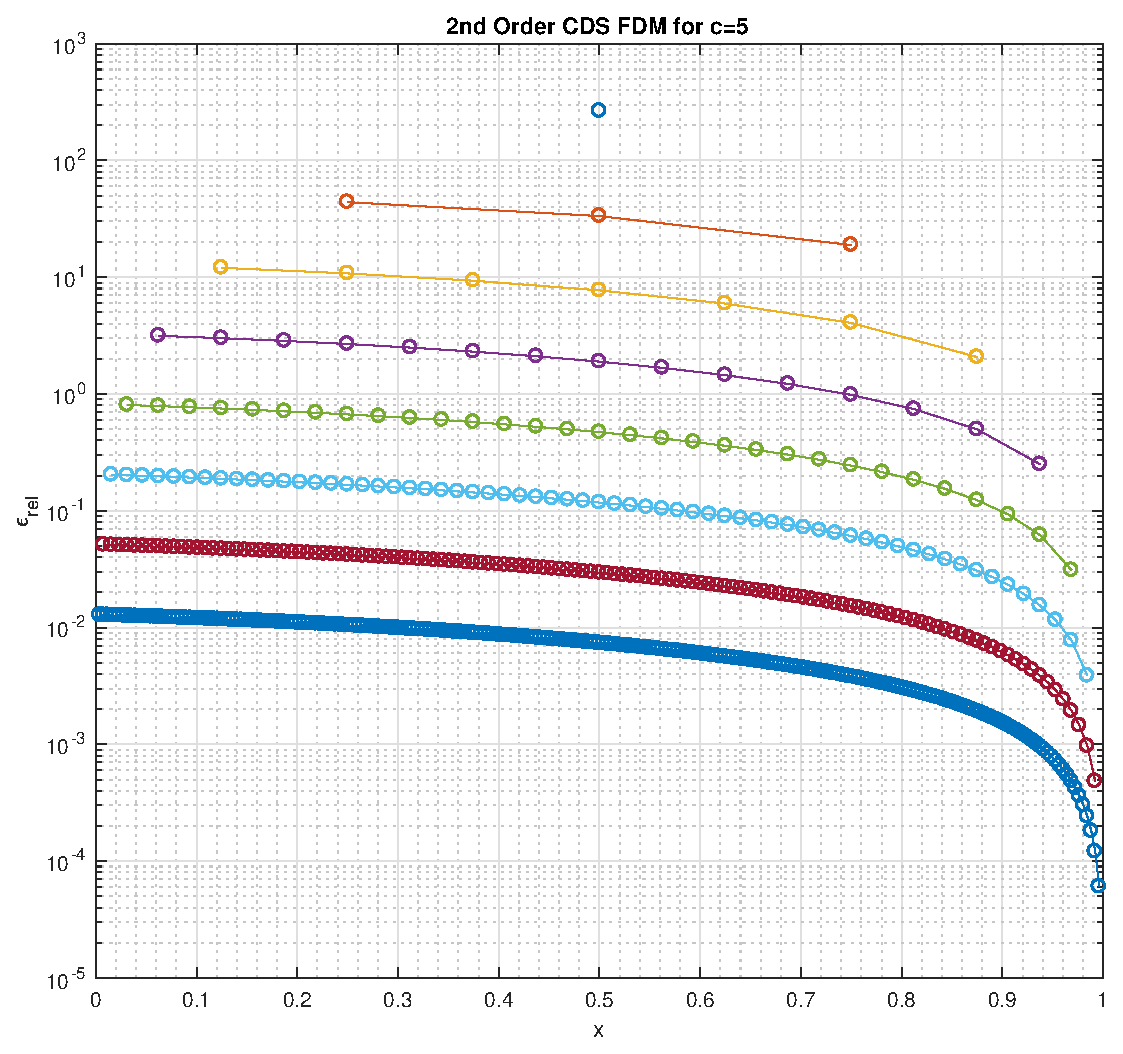
\includegraphics[width = 0.31\linewidth]{pointwise_error_2nd_order_cds_c_5}
		\caption{2nd-Order CDS FDM and Pointwise Error for Convection-Diffusion Equation with $c = 5$}
	\end{center}
\end{figure}

\newpage

\begin{figure}[H]
	\begin{center}
		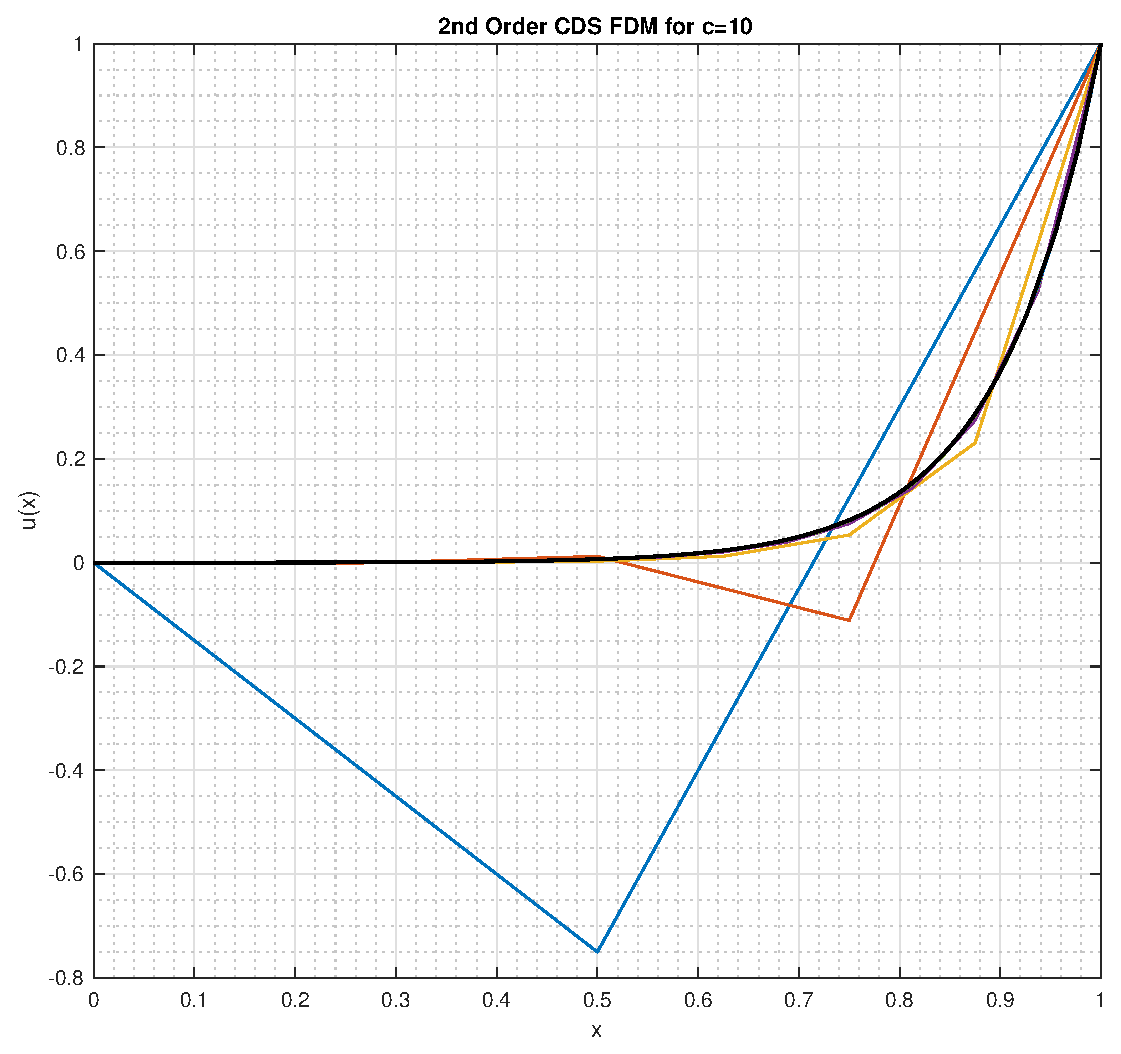
\includegraphics[width = 0.31\linewidth]{solution_2nd_order_cds_c_10}
		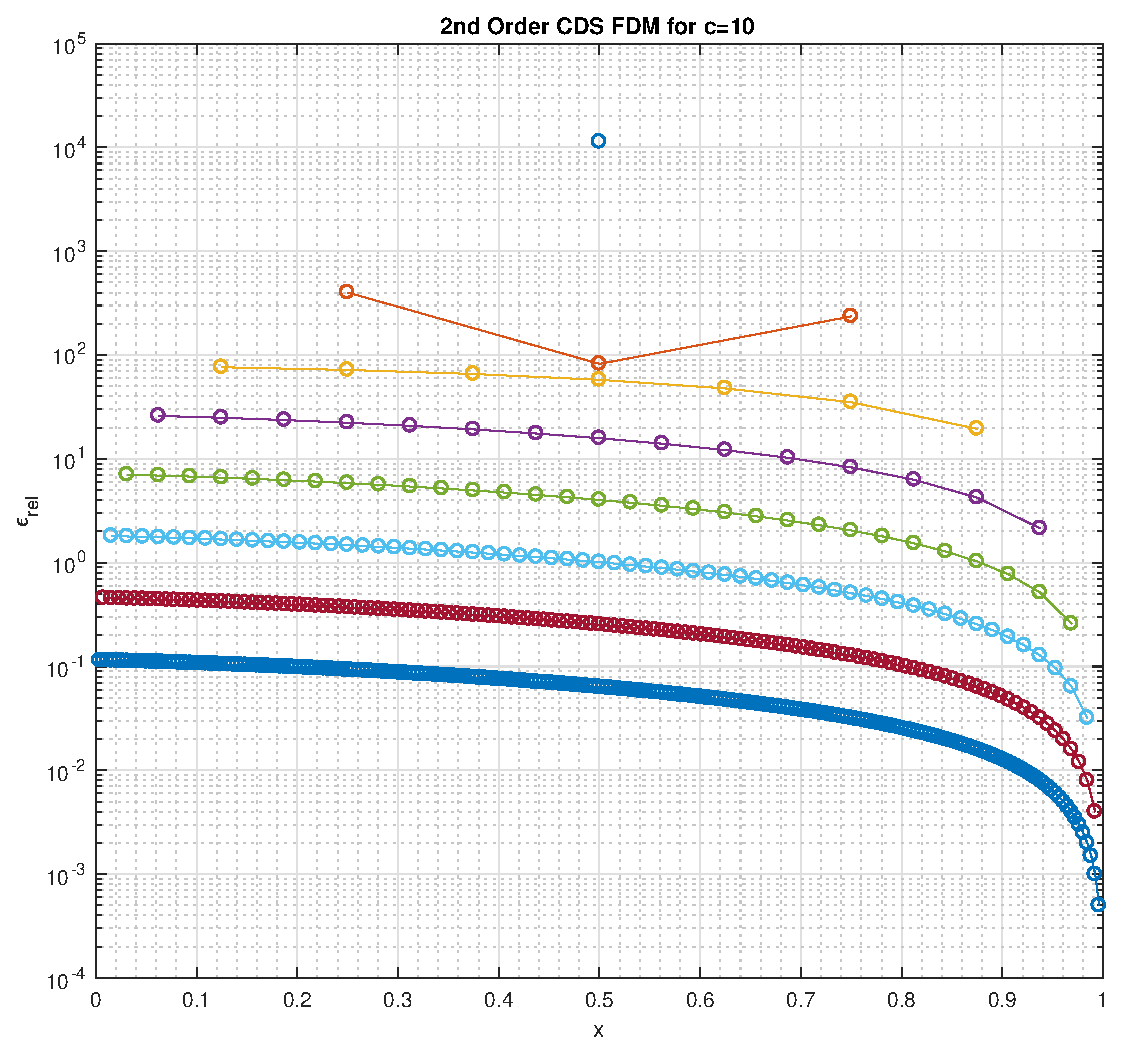
\includegraphics[width = 0.31\linewidth]{pointwise_error_2nd_order_cds_c_10}
		\caption{2nd-Order CDS FDM and Pointwise Error for Convection-Diffusion Equation with $c = 10$}
	\end{center}
\end{figure}

\begin{figure}[H]
	\begin{center}
		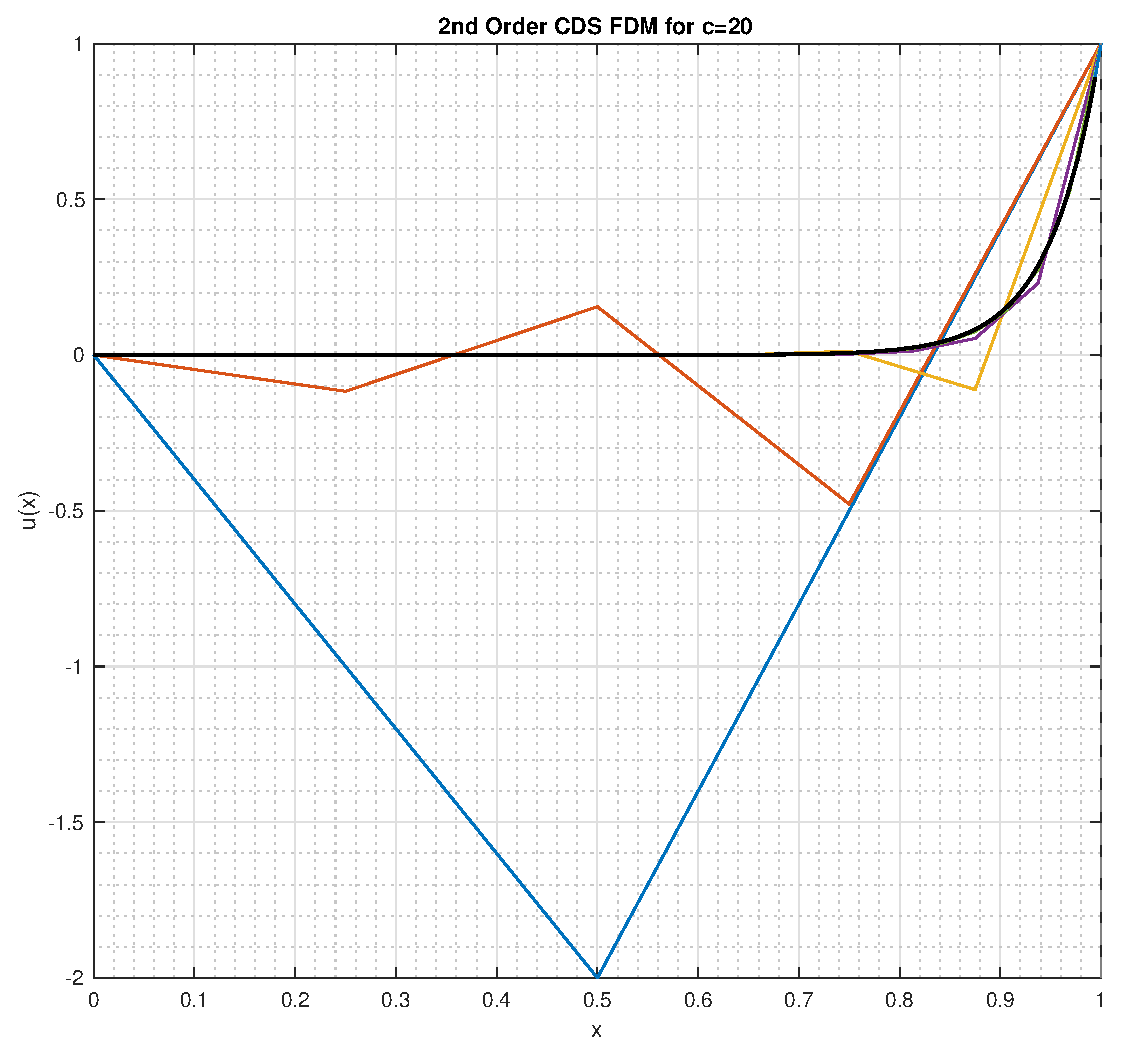
\includegraphics[width = 0.31\linewidth]{solution_2nd_order_cds_c_20}
		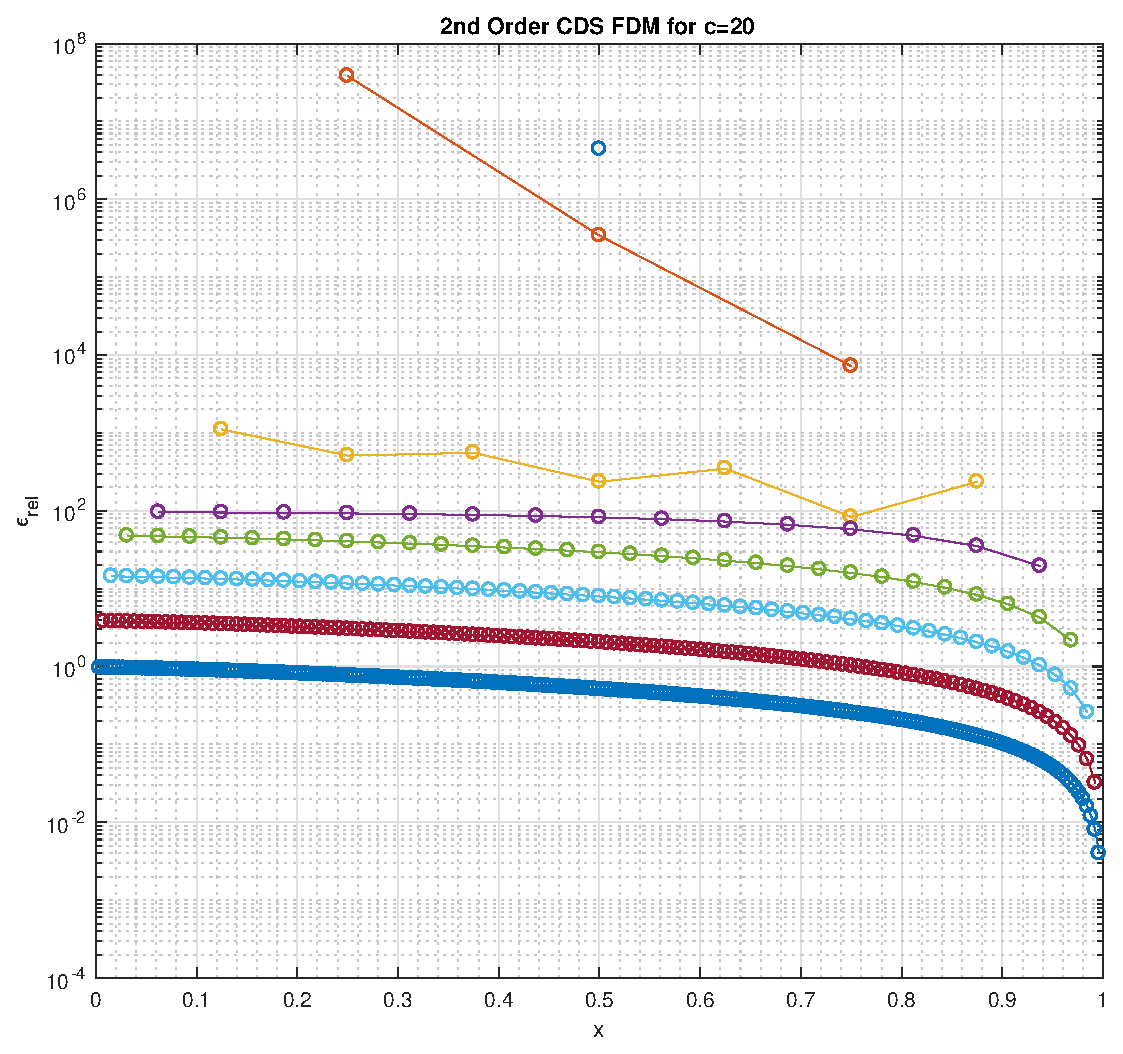
\includegraphics[width = 0.31\linewidth]{pointwise_error_2nd_order_cds_c_20}
		\caption{2nd-Order CDS FDM and Pointwise Error for Convection-Diffusion Equation with $c = 20$}
	\end{center}
\end{figure}

\begin{figure}[H]
	\begin{center}
		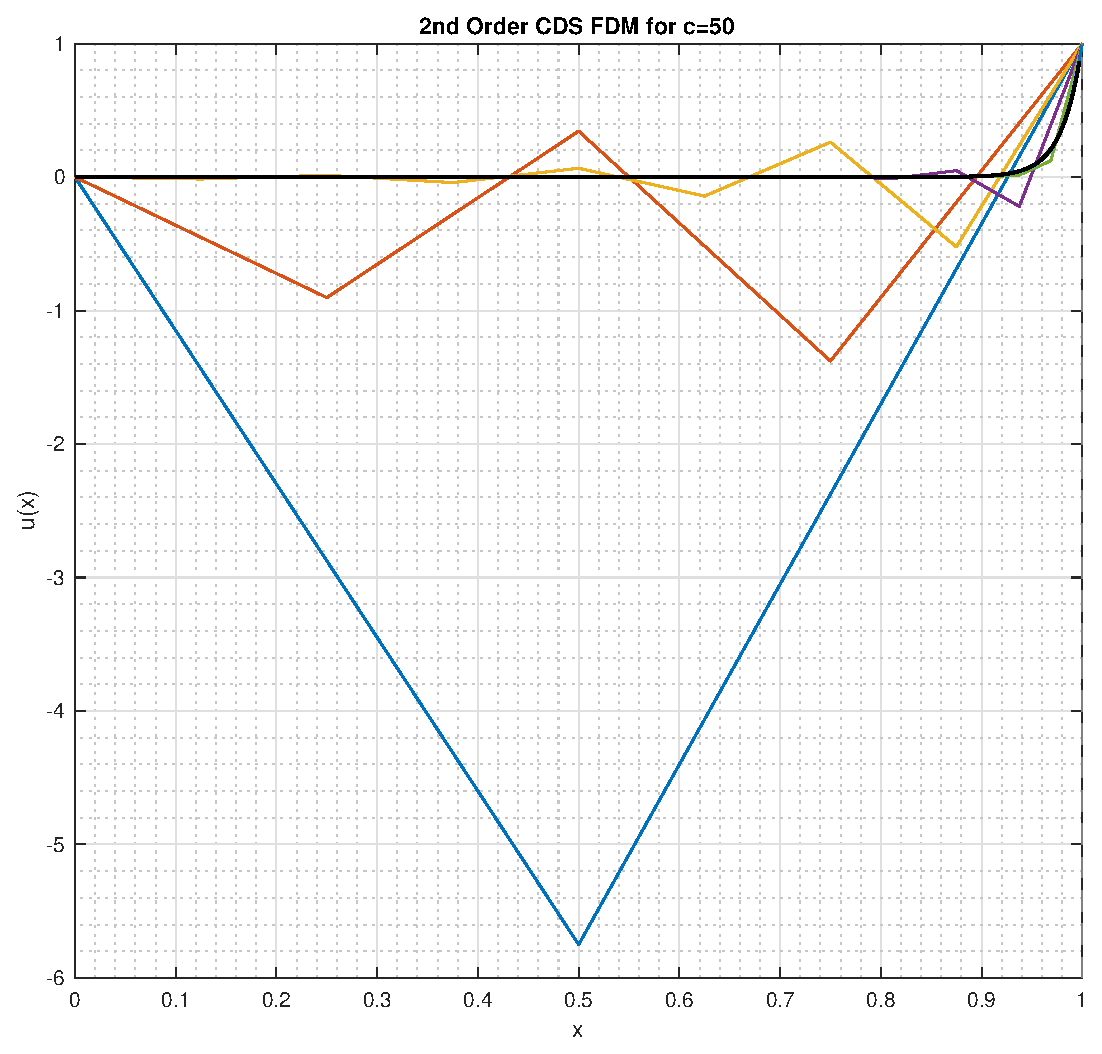
\includegraphics[width = 0.31\linewidth]{solution_2nd_order_cds_c_50}
		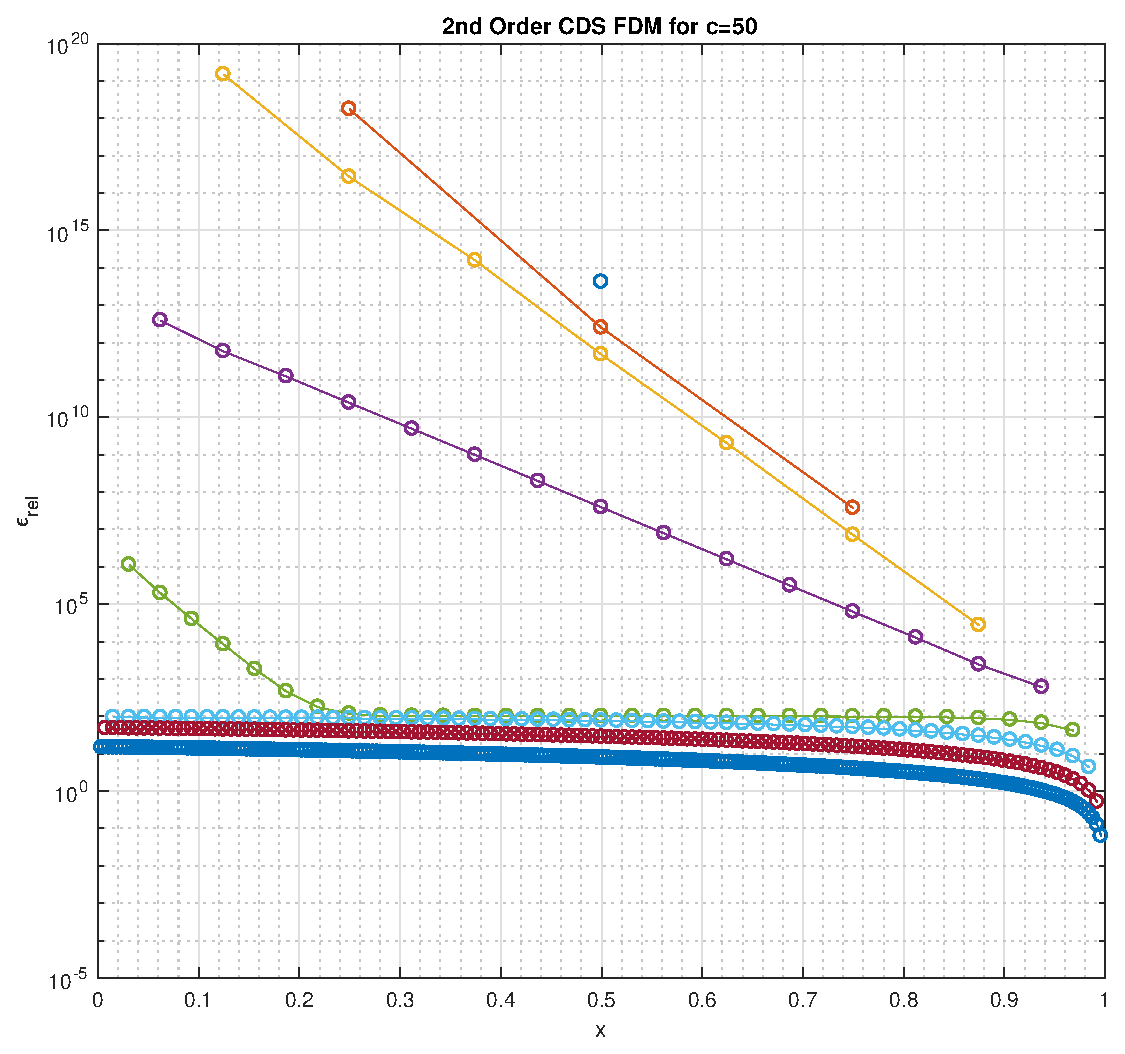
\includegraphics[width = 0.31\linewidth]{pointwise_error_2nd_order_cds_c_50}
		\caption{2nd-Order CDS FDM and Pointwise Error for Convection-Diffusion Equation with $c = 50$}
	\end{center}
\end{figure}

\begin{center}
	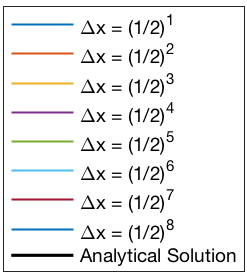
\includegraphics[height = 0.11\linewidth]{legend}
\end{center}

\newpage

\subsubsection{4th-Order Central Difference Scheme - Diffusion Equation}

\begin{figure}[H]
	\begin{center}
		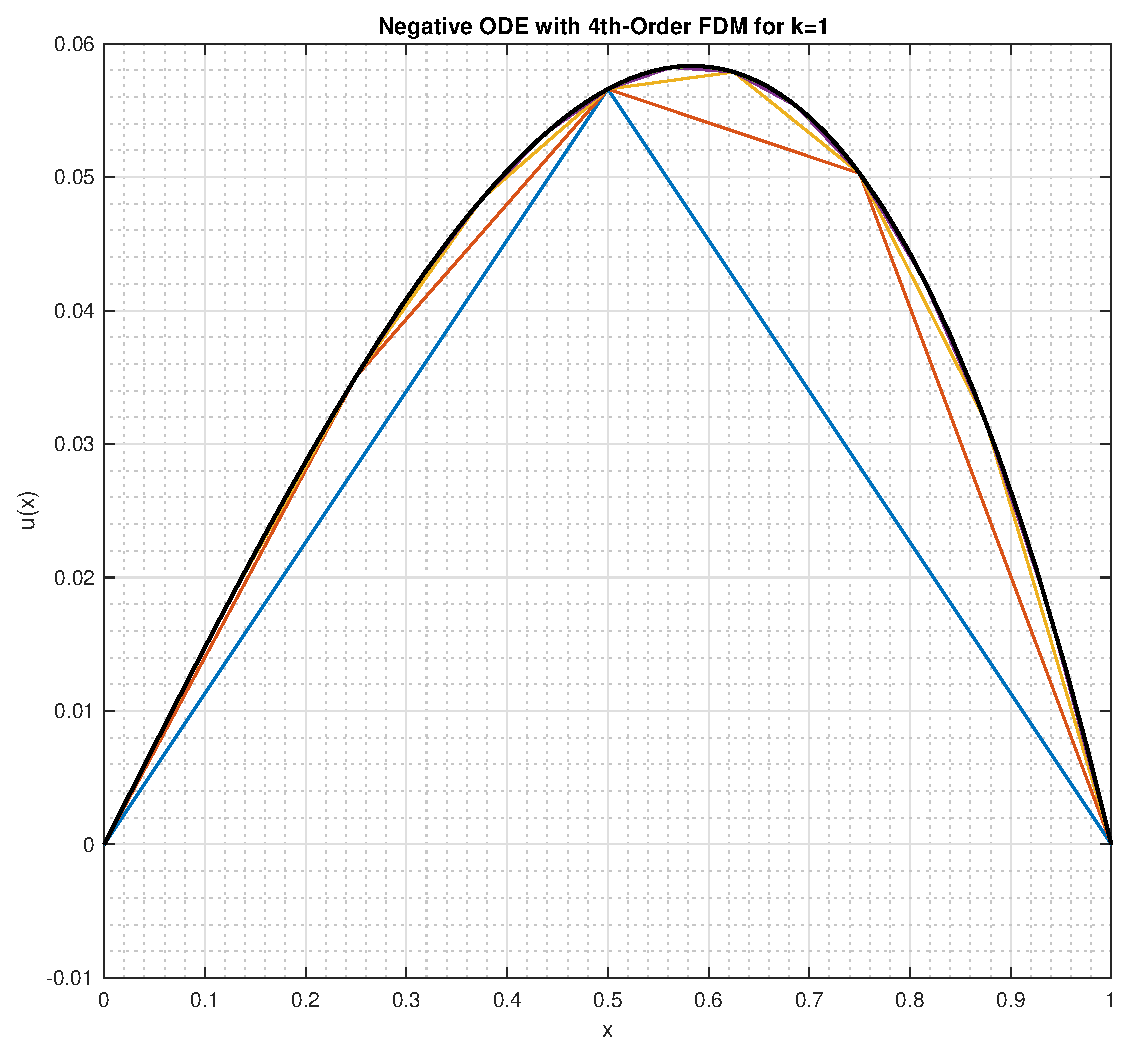
\includegraphics[width = 0.31\linewidth]{negative_ode_order_4_k_1}
		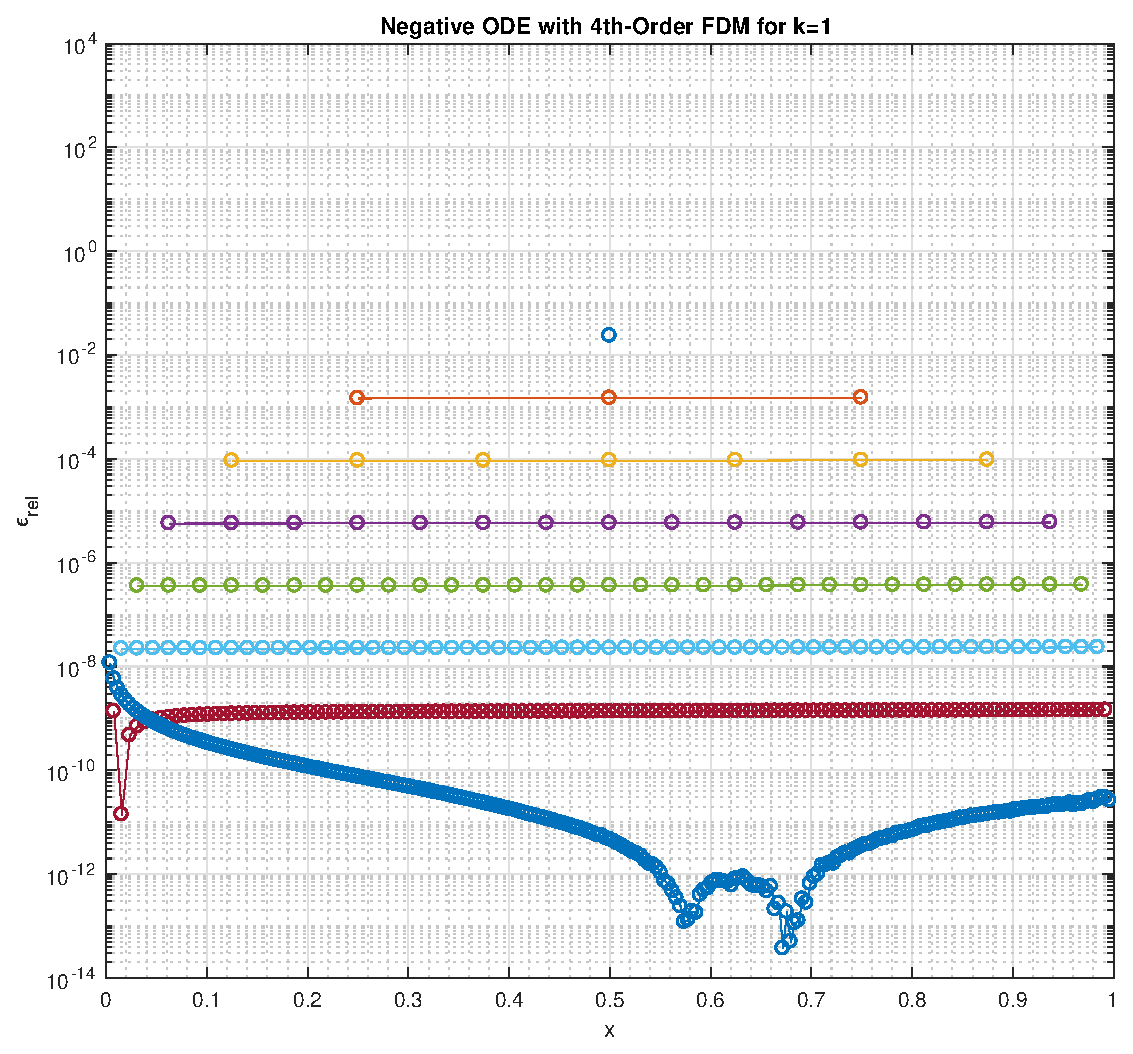
\includegraphics[width = 0.31\linewidth]{error_negative_ode_order_4_k_1}
		\caption{4th-Order CDS FDM and Pointwise Error for Diffusion Equation with $k = 1$}
	\end{center}
\end{figure}

\begin{figure}[H]
	\begin{center}
		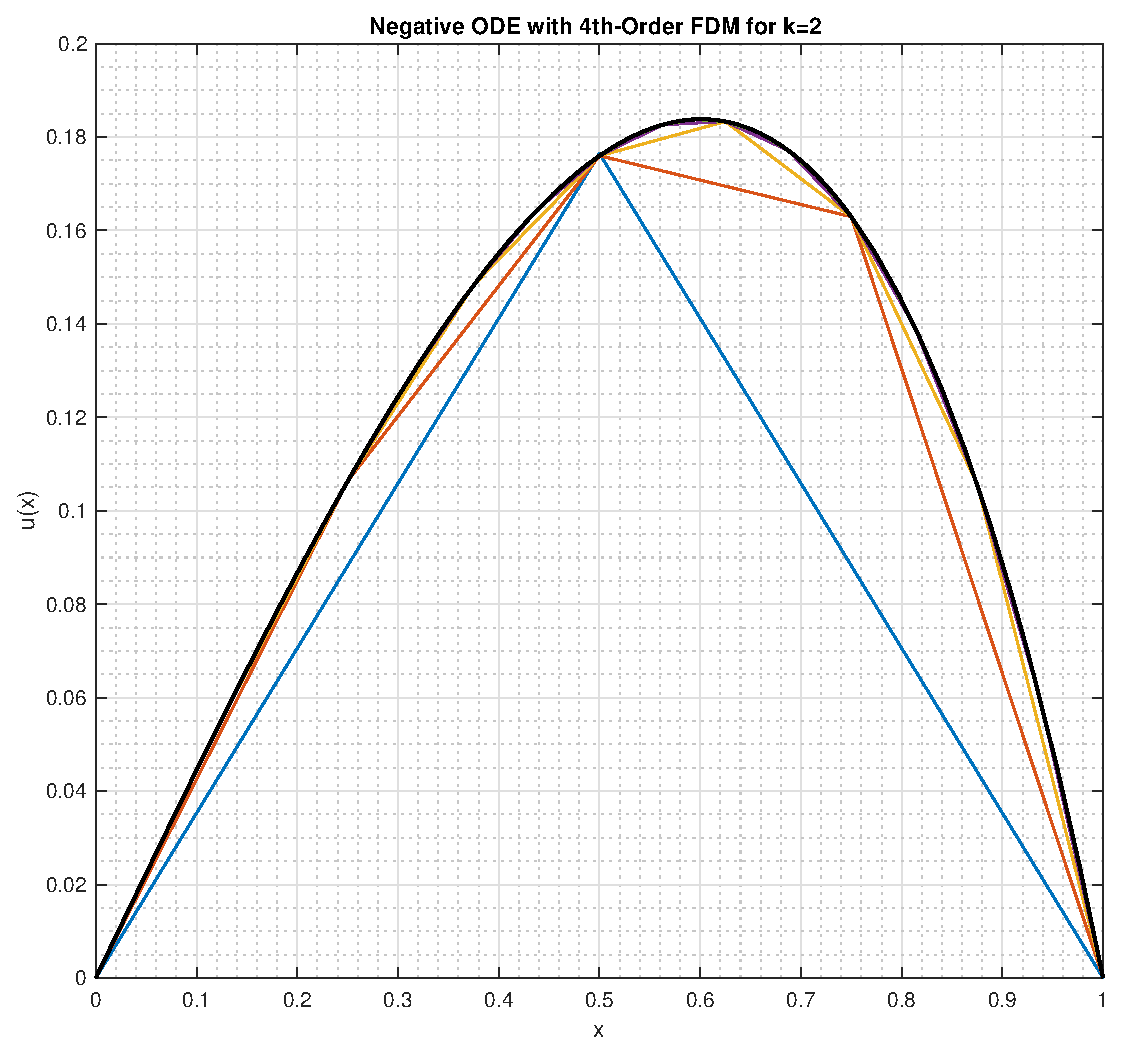
\includegraphics[width = 0.31\linewidth]{negative_ode_order_4_k_2}
		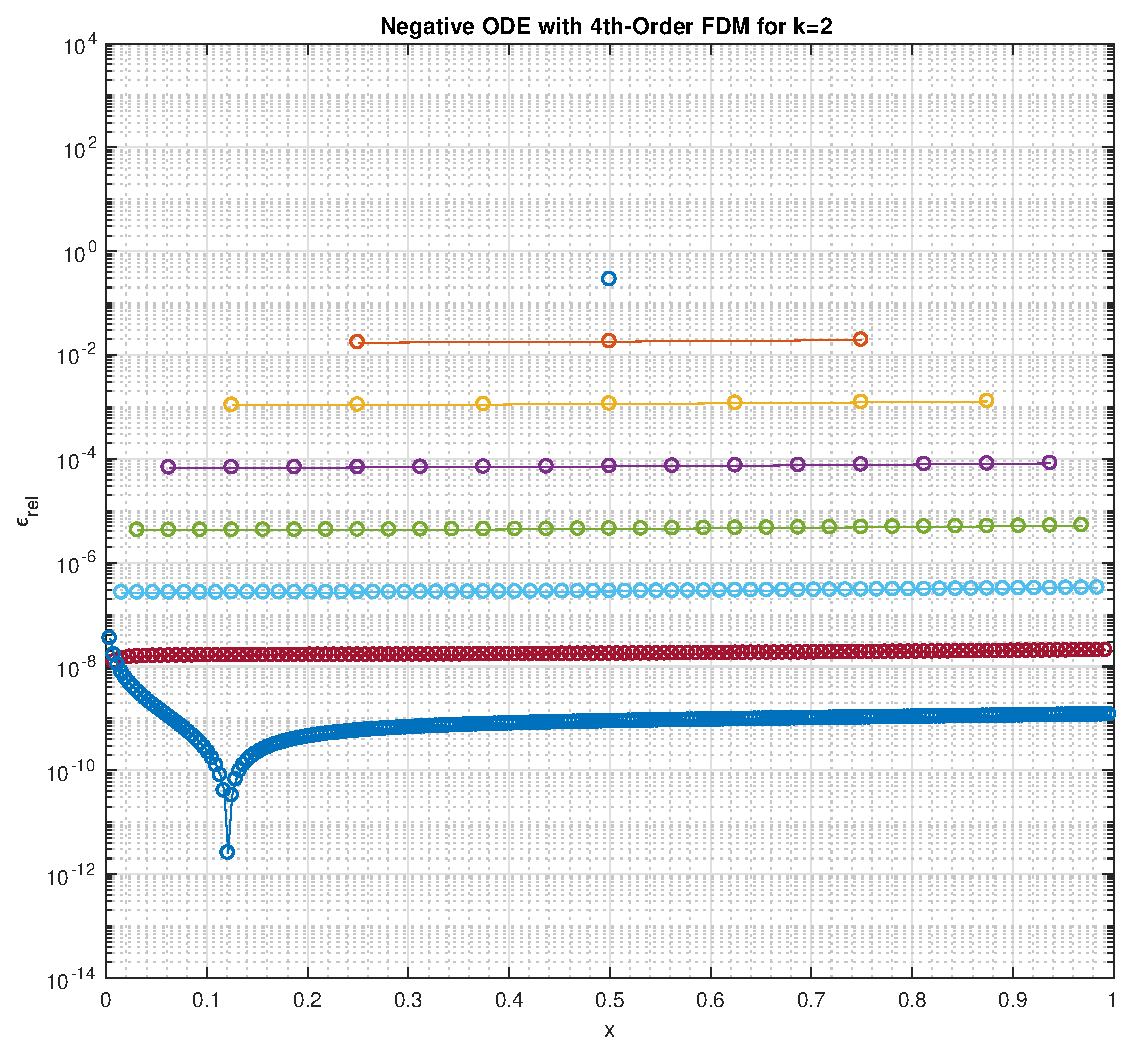
\includegraphics[width = 0.31\linewidth]{error_negative_ode_order_4_k_2}
		\caption{4th-Order CDS FDM and Pointwise Error for Diffusion Equation with $k = 2$}
	\end{center}
\end{figure}

\begin{figure}[H]
	\begin{center}
		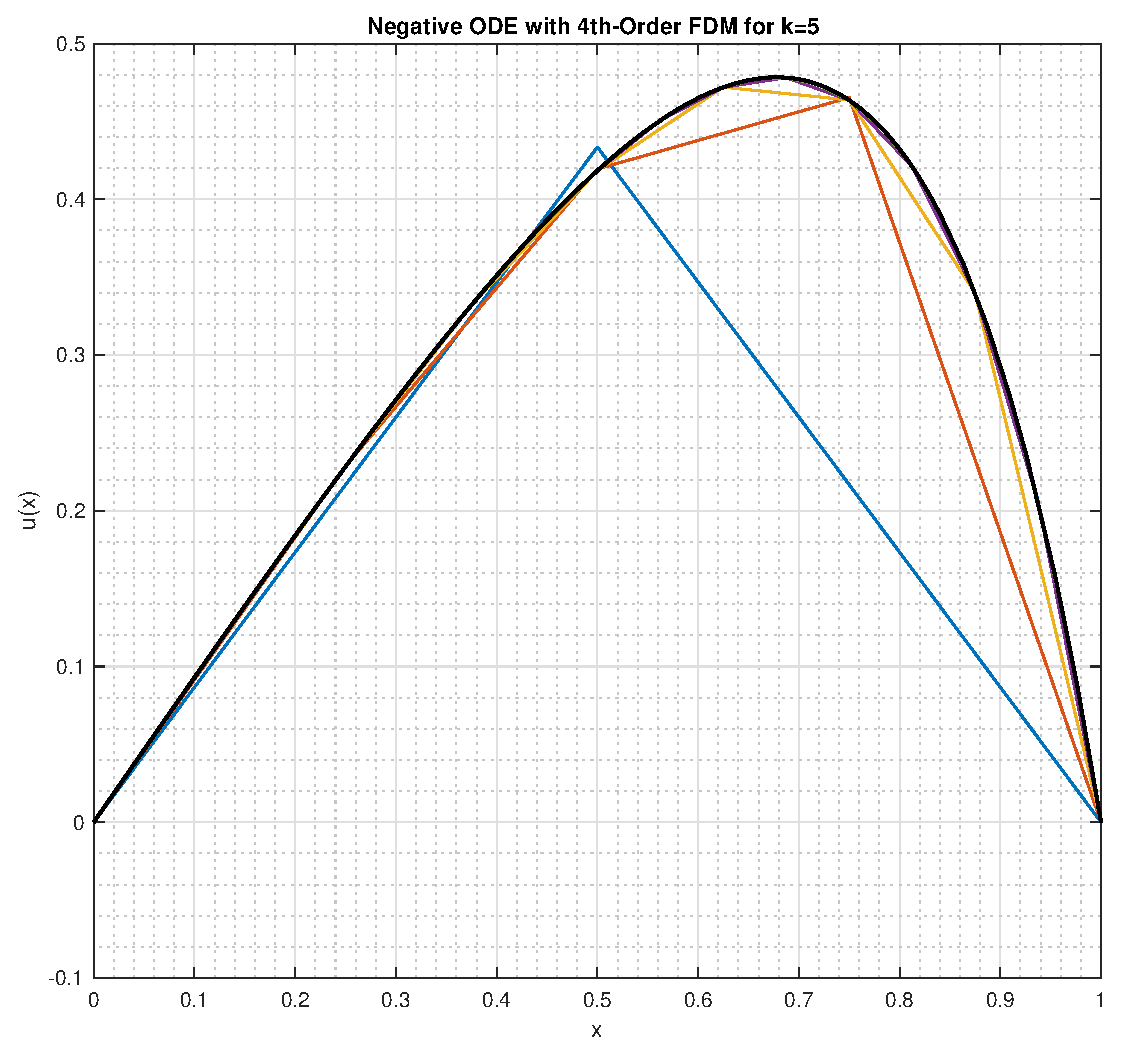
\includegraphics[width = 0.31\linewidth]{negative_ode_order_4_k_5}
		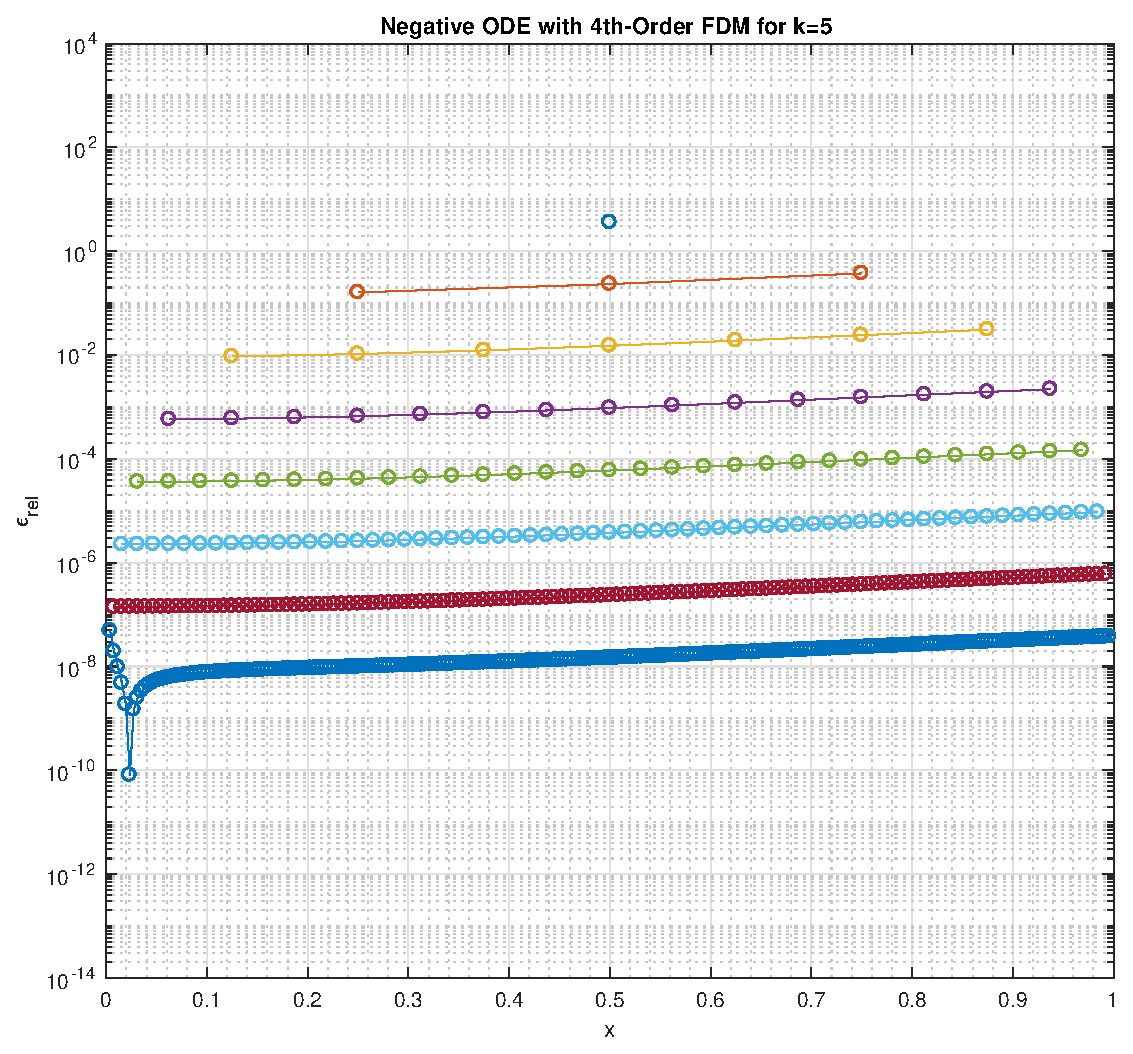
\includegraphics[width = 0.31\linewidth]{error_negative_ode_order_4_k_5}
		\caption{4th-Order CDS FDM and Pointwise Error for Diffusion Equation with $k = 5$}
	\end{center}
\end{figure}

\newpage

\begin{figure}[H]
	\begin{center}
		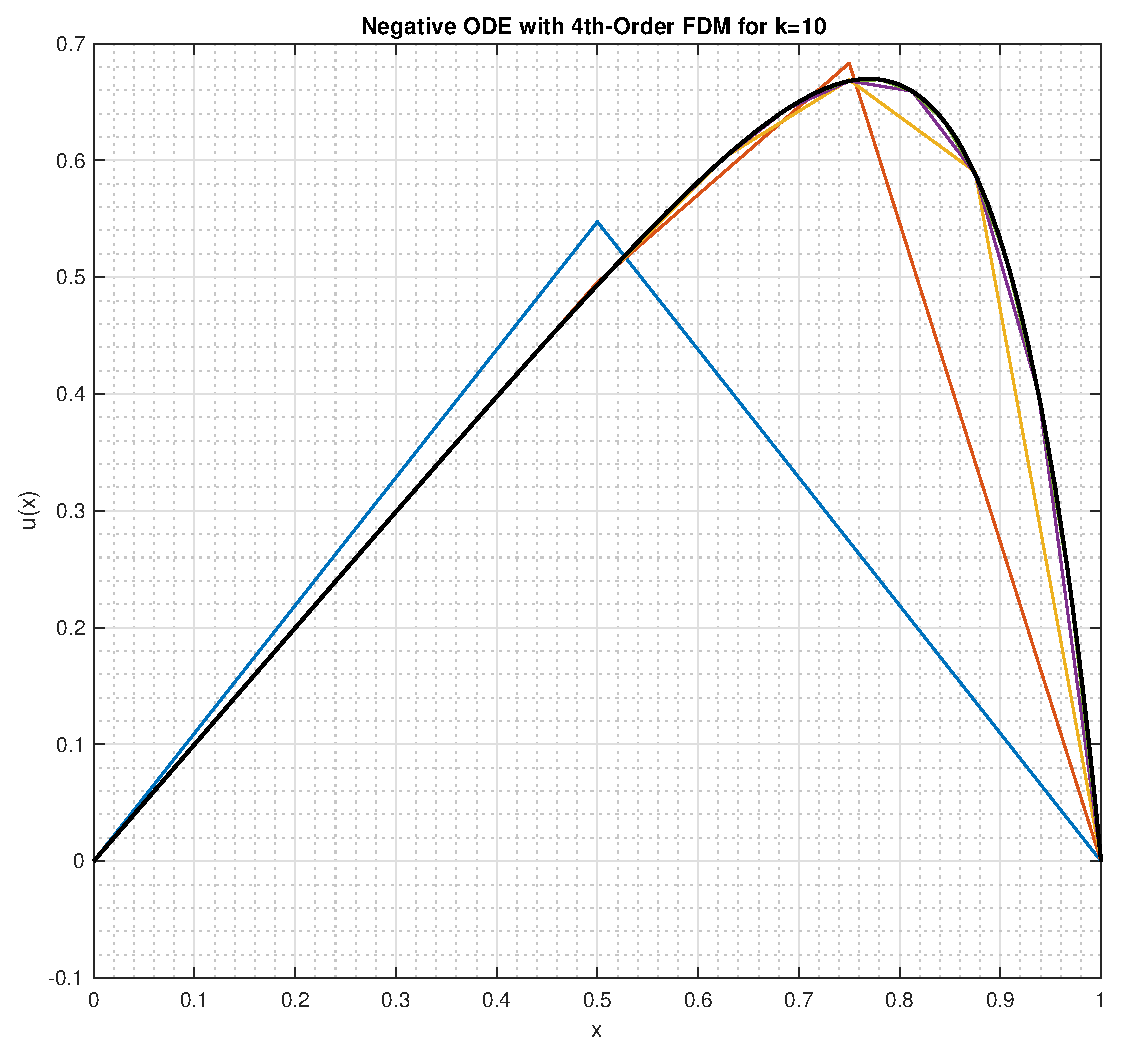
\includegraphics[width = 0.31\linewidth]{negative_ode_order_4_k_10}
		\includegraphics[width = 0.31\linewidth]{error_negative_ode_order_4_k_10}
		\caption{4th-Order CDS FDM and Pointwise Error for Diffusion Equation with $k = 10$}
	\end{center}
\end{figure}

\begin{figure}[H]
	\begin{center}
		\includegraphics[width = 0.31\linewidth]{negative_ode_order_4_k_20}
		\includegraphics[width = 0.31\linewidth]{error_negative_ode_order_4_k_20}
		\caption{4th-Order CDS FDM and Pointwise Error for Diffusion Equation with $k = 20$}
	\end{center}
\end{figure}

\begin{figure}[H]
	\begin{center}
		\includegraphics[width = 0.31\linewidth]{negative_ode_order_4_k_50}
		\includegraphics[width = 0.31\linewidth]{error_negative_ode_order_4_k_50}
		\caption{4th-Order CDS FDM and Pointwise Error for Diffusion Equation with $k = 50$}
	\end{center}
\end{figure}

\begin{center}
	\includegraphics[height = 0.19\linewidth]{legend}
\end{center}

\newpage

\subsubsection{4th-Order Central Difference Scheme - Harmonic Wave Equation}

\begin{figure}[H]
	\begin{center}
		\includegraphics[width = 0.31\linewidth]{positive_ode_order_4_k_1}
		\includegraphics[width = 0.31\linewidth]{error_positive_ode_order_4_k_1}
		\caption{4th-Order CDS FDM and Pointwise Error for Harmonic Wave Equation with $k = 1$}
	\end{center}
\end{figure}

\begin{figure}[H]
	\begin{center}
		\includegraphics[width = 0.31\linewidth]{positive_ode_order_4_k_2}
		\includegraphics[width = 0.31\linewidth]{error_positive_ode_order_4_k_2}
		\caption{4th-Order CDS FDM and Pointwise Error for Harmonic Wave Equation with $k = 2$}
	\end{center}
\end{figure}

\begin{figure}[H]
	\begin{center}
		\includegraphics[width = 0.31\linewidth]{positive_ode_order_4_k_5}
		\includegraphics[width = 0.31\linewidth]{error_positive_ode_order_4_k_5}
		\caption{4th-Order CDS FDM and Pointwise Error for Harmonic Wave Equation with $k = 5$}
	\end{center}
\end{figure}

\newpage

\begin{figure}[H]
	\begin{center}
		\includegraphics[width = 0.31\linewidth]{positive_ode_order_4_k_10}
		\includegraphics[width = 0.31\linewidth]{error_positive_ode_order_4_k_10}
		\caption{4th-Order CDS FDM and Pointwise Error for Harmonic Wave Equation with $k = 10$}
	\end{center}
\end{figure}

\begin{figure}[H]
	\begin{center}
		\includegraphics[width = 0.31\linewidth]{positive_ode_order_4_k_20}
		\includegraphics[width = 0.31\linewidth]{error_positive_ode_order_4_k_20}
		\caption{4th-Order CDS FDM and Pointwise Error for Harmonic Wave Equation with $k = 20$}
	\end{center}
\end{figure}

\begin{figure}[H]
	\begin{center}
		\includegraphics[width = 0.31\linewidth]{positive_ode_order_4_k_50}
		\includegraphics[width = 0.31\linewidth]{error_positive_ode_order_4_k_50}
		\caption{4th-Order CDS FDM and Pointwise Error for Harmonic Wave Equation with $k = 50$}
	\end{center}
\end{figure}

\begin{center}
	\includegraphics[height = 0.11\linewidth]{legend}
\end{center}

\newpage

\subsubsection{4th-Order Central Difference Scheme - Convection-Diffusion Equation}

\begin{figure}[H]
	\begin{center}
		\includegraphics[width = 0.31\linewidth]{solution_4th_order_cds_c_1}
		\includegraphics[width = 0.31\linewidth]{pointwise_error_4th_order_cds_c_1}
		\caption{4th-Order CDS FDM and Pointwise Error for Convection-Diffusion Equation with $c = 1$}
	\end{center}
\end{figure}

\begin{figure}[H]
	\begin{center}
		\includegraphics[width = 0.31\linewidth]{solution_4th_order_cds_c_2}
		\includegraphics[width = 0.31\linewidth]{pointwise_error_4th_order_cds_c_2}
		\caption{4th-Order CDS FDM and Pointwise Error for Convection-Diffusion Equation with $c = 2$}
	\end{center}
\end{figure}

\begin{figure}[H]
	\begin{center}
		\includegraphics[width = 0.31\linewidth]{solution_4th_order_cds_c_5}
		\includegraphics[width = 0.31\linewidth]{pointwise_error_4th_order_cds_c_5}
		\caption{4th-Order CDS FDM and Pointwise Error for Convection-Diffusion Equation with $c = 5$}
	\end{center}
\end{figure}

\newpage

\begin{figure}[H]
	\begin{center}
		\includegraphics[width = 0.31\linewidth]{solution_4th_order_cds_c_10}
		\includegraphics[width = 0.31\linewidth]{pointwise_error_4th_order_cds_c_10}
		\caption{4th-Order CDS FDM and Pointwise Error for Convection-Diffusion Equation with $c = 10$}
	\end{center}
\end{figure}

\begin{figure}[H]
	\begin{center}
		\includegraphics[width = 0.31\linewidth]{solution_4th_order_cds_c_20}
		\includegraphics[width = 0.31\linewidth]{pointwise_error_4th_order_cds_c_20}
		\caption{4th-Order CDS FDM and Pointwise Error for Convection-Diffusion Equation with $c = 20$}
	\end{center}
\end{figure}

\begin{figure}[H]
	\begin{center}
		\includegraphics[width = 0.31\linewidth]{solution_4th_order_cds_c_50}
		\includegraphics[width = 0.31\linewidth]{pointwise_error_4th_order_cds_c_50}
		\caption{4th-Order CDS FDM and Pointwise Error for Convection-Diffusion Equation with $c = 50$}
	\end{center}
\end{figure}

\begin{center}
	\includegraphics[height = 0.11\linewidth]{legend}
\end{center}

\newpage

\subsection{Finite Element Method -- Solution Results}

\subsubsection{1st-Order (p=1) Galerkin Method - Diffusion Equation}

\begin{figure}[H]
	\begin{center}
		\includegraphics[width = 0.31\linewidth]{solution_diffusion_p_1_k_1}
		\includegraphics[width = 0.31\linewidth]{pointwise_error_diffusion_p_1_k_1}
		\caption{1st-Order (p=1) Galerkin Method FEM and Pointwise Error for Diffusion Equation with $k = 1$}
	\end{center}
\end{figure}

\begin{figure}[H]
	\begin{center}
		\includegraphics[width = 0.31\linewidth]{solution_diffusion_p_1_k_2}
		\includegraphics[width = 0.31\linewidth]{pointwise_error_diffusion_p_1_k_2}
		\caption{1st-Order (p=1) Galerkin Method FEM and Pointwise Error for Diffusion Equation with $k = 2$}
	\end{center}
\end{figure}

\begin{figure}[H]
	\begin{center}
		\includegraphics[width = 0.31\linewidth]{solution_diffusion_p_1_k_5}
		\includegraphics[width = 0.31\linewidth]{pointwise_error_diffusion_p_1_k_5}
		\caption{1st-Order (p=1) Galerkin Method FEM and Pointwise Error for Diffusion Equation with $k = 5$}
	\end{center}
\end{figure}

\newpage

\begin{figure}[H]
	\begin{center}
		\includegraphics[width = 0.31\linewidth]{solution_diffusion_p_1_k_10}
		\includegraphics[width = 0.31\linewidth]{pointwise_error_diffusion_p_1_k_10}
		\caption{1st-Order (p=1) Galerkin Method FEM and Pointwise Error for Diffusion Equation with $k = 10$}
	\end{center}
\end{figure}

\begin{figure}[H]
	\begin{center}
		\includegraphics[width = 0.31\linewidth]{solution_diffusion_p_1_k_20}
		\includegraphics[width = 0.31\linewidth]{pointwise_error_diffusion_p_1_k_20}
		\caption{1st-Order (p=1) Galerkin Method FEM and Pointwise Error for Diffusion Equation with $k = 20$}
	\end{center}
\end{figure}

\begin{figure}[H]
	\begin{center}
		\includegraphics[width = 0.31\linewidth]{solution_diffusion_p_1_k_50}
		\includegraphics[width = 0.31\linewidth]{pointwise_error_diffusion_p_1_k_50}
		\caption{1st-Order (p=1) Galerkin Method FEM and Pointwise Error for Diffusion Equation with $k = 50$}
	\end{center}
\end{figure}

\begin{center}
	\includegraphics[height = 0.11\linewidth]{legend}
\end{center}

\newpage

\subsubsection{1st-Order (p=1) Galerkin Method - Harmonic Wave Equation}

\begin{figure}[H]
	\begin{center}
		\includegraphics[width = 0.31\linewidth]{solution_harmonic_p_1_k_1}
		\includegraphics[width = 0.31\linewidth]{pointwise_error_harmonic_p_1_k_1}
		\caption{1st-Order (p=1) Galerkin Method FEM and Pointwise Error for Harmonic Wave Equation with $k = 1$}
	\end{center}
\end{figure}

\begin{figure}[H]
	\begin{center}
		\includegraphics[width = 0.31\linewidth]{solution_harmonic_p_1_k_2}
		\includegraphics[width = 0.31\linewidth]{pointwise_error_harmonic_p_1_k_2}
		\caption{1st-Order (p=1) Galerkin Method FEM and Pointwise Error for Harmonic Wave Equation with $k = 2$}
	\end{center}
\end{figure}

\begin{figure}[H]
	\begin{center}
		\includegraphics[width = 0.31\linewidth]{solution_harmonic_p_1_k_5}
		\includegraphics[width = 0.31\linewidth]{pointwise_error_harmonic_p_1_k_5}
		\caption{1st-Order (p=1) Galerkin Method FEM and Pointwise Error for Harmonic Wave Equation with $k = 5$}
	\end{center}
\end{figure}

\newpage

\begin{figure}[H]
	\begin{center}
		\includegraphics[width = 0.31\linewidth]{solution_harmonic_p_1_k_10}
		\includegraphics[width = 0.31\linewidth]{pointwise_error_harmonic_p_1_k_10}
		\caption{1st-Order (p=1) Galerkin Method FEM and Pointwise Error for Harmonic Wave Equation with $k = 10$}
	\end{center}
\end{figure}

\begin{figure}[H]
	\begin{center}
		\includegraphics[width = 0.31\linewidth]{solution_harmonic_p_1_k_20}
		\includegraphics[width = 0.31\linewidth]{pointwise_error_harmonic_p_1_k_20}
		\caption{1st-Order (p=1) Galerkin Method FEM and Pointwise Error for Harmonic Wave Equation with $k = 20$}
	\end{center}
\end{figure}

\begin{figure}[H]
	\begin{center}
		\includegraphics[width = 0.31\linewidth]{solution_harmonic_p_1_k_50}
		\includegraphics[width = 0.31\linewidth]{pointwise_error_harmonic_p_1_k_50}
		\caption{1st-Order (p=1) Galerkin Method FEM and Pointwise Error for Harmonic Wave Equation with $k = 50$}
	\end{center}
\end{figure}

\begin{center}
	\includegraphics[height = 0.10\linewidth]{legend}
\end{center}

\newpage

\subsubsection{1st-Order (p=1) Galerkin Method - Convection-Diffusion Equation}

\begin{figure}[H]
	\begin{center}
		\includegraphics[width = 0.31\linewidth]{solution_convection_p_1_k_1}
		\includegraphics[width = 0.31\linewidth]{pointwise_error_convection_p_1_k_1}
		\caption{1st-Order (p=1) Galerkin Method FEM and Pointwise Error for Convection-Diffusion Equation with $c = 1$}
	\end{center}
\end{figure}

\begin{figure}[H]
	\begin{center}
		\includegraphics[width = 0.31\linewidth]{solution_convection_p_1_k_2}
		\includegraphics[width = 0.31\linewidth]{pointwise_error_convection_p_1_k_2}
		\caption{1st-Order (p=1) Galerkin Method FEM and Pointwise Error for Convection-Diffusion Equation with $c = 2$}
	\end{center}
\end{figure}

\begin{figure}[H]
	\begin{center}
		\includegraphics[width = 0.31\linewidth]{solution_convection_p_1_k_5}
		\includegraphics[width = 0.31\linewidth]{pointwise_error_convection_p_1_k_5}
		\caption{1st-Order (p=1) Galerkin Method FEM and Pointwise Error for Convection-Diffusion Equation with $c = 5$}
	\end{center}
\end{figure}

\newpage

\begin{figure}[H]
	\begin{center}
		\includegraphics[width = 0.31\linewidth]{solution_convection_p_1_k_10}
		\includegraphics[width = 0.31\linewidth]{pointwise_error_convection_p_1_k_10}
		\caption{1st-Order (p=1) Galerkin Method FEM and Pointwise Error for Convection-Diffusion Equation with $c = 10$}
	\end{center}
\end{figure}

\begin{figure}[H]
	\begin{center}
		\includegraphics[width = 0.31\linewidth]{solution_convection_p_1_k_20}
		\includegraphics[width = 0.31\linewidth]{pointwise_error_convection_p_1_k_20}
		\caption{1st-Order (p=1) Galerkin Method FEM and Pointwise Error for Convection-Diffusion Equation with $c = 20$}
	\end{center}
\end{figure}

\begin{figure}[H]
	\begin{center}
		\includegraphics[width = 0.31\linewidth]{solution_convection_p_1_k_50}
		\includegraphics[width = 0.31\linewidth]{pointwise_error_convection_p_1_k_50}
		\caption{1st-Order (p=1) Galerkin Method FEM and Pointwise Error for Convection-Diffusion Equation with $c = 50$}
	\end{center}
\end{figure}

\begin{center}
	\includegraphics[height = 0.11\linewidth]{legend}
\end{center}

\subsubsection{2nd-Order (p=2) Galerkin Method - Diffusion Equation}

\begin{figure}[H]
	\begin{center}
		%\includegraphics[width = 0.31\linewidth]{solution_diffusion_p_2_k_1}
		%\includegraphics[width = 0.31\linewidth]{pointwise_error_diffusion_p_2_k_1}
		\caption{2nd-Order (p=2) Galerkin Method FEM and Pointwise Error for Diffusion Equation with $k = 1$}
	\end{center}
\end{figure}

\begin{figure}[H]
	\begin{center}
		%\includegraphics[width = 0.31\linewidth]{solution_diffusion_p_2_k_2}
		%\includegraphics[width = 0.31\linewidth]{pointwise_error_diffusion_p_2_k_2}
		\caption{2nd-Order (p=2) Galerkin Method FEM and Pointwise Error for Diffusion Equation with $k = 2$}
	\end{center}
\end{figure}

\begin{figure}[H]
	\begin{center}
		%\includegraphics[width = 0.31\linewidth]{solution_diffusion_p_2_k_5}
		%\includegraphics[width = 0.31\linewidth]{pointwise_error_diffusion_p_2_k_5}
		\caption{2nd-Order (p=2) Galerkin Method FEM and Pointwise Error for Diffusion Equation with $k = 5$}
	\end{center}
\end{figure}

\newpage

\begin{figure}[H]
	\begin{center}
		%\includegraphics[width = 0.31\linewidth]{solution_diffusion_p_2_k_10}
		%\includegraphics[width = 0.31\linewidth]{pointwise_error_diffusion_p_2_k_10}
		\caption{2nd-Order (p=2) Galerkin Method FEM and Pointwise Error for Diffusion Equation with $k = 10$}
	\end{center}
\end{figure}

\begin{figure}[H]
	\begin{center}
		%\includegraphics[width = 0.31\linewidth]{solution_diffusion_p_2_k_20}
		%\includegraphics[width = 0.31\linewidth]{pointwise_error_diffusion_p_2_k_20}
		\caption{2nd-Order (p=2) Galerkin Method FEM and Pointwise Error for Diffusion Equation with $k = 20$}
	\end{center}
\end{figure}

\begin{figure}[H]
	\begin{center}
		%\includegraphics[width = 0.31\linewidth]{solution_diffusion_p_2_k_50}
		%\includegraphics[width = 0.31\linewidth]{pointwise_error_diffusion_p_2_k_50}
		\caption{2nd-Order (p=2) Galerkin Method FEM and Pointwise Error for Diffusion Equation with $k = 50$}
	\end{center}
\end{figure}

\begin{center}
	\includegraphics[height = 0.11\linewidth]{legend}
\end{center}

\newpage

\subsubsection{2nd-Order (p=2) Galerkin Method - Harmonic Wave Equation}

\begin{figure}[H]
	\begin{center}
		%\includegraphics[width = 0.31\linewidth]{solution_harmonic_p_2_k_1}
		%\includegraphics[width = 0.31\linewidth]{pointwise_error_harmonic_p_2_k_1}
		\caption{2nd-Order (p=2) Galerkin Method FEM and Pointwise Error for Harmonic Wave Equation with $k = 1$}
	\end{center}
\end{figure}

\begin{figure}[H]
	\begin{center}
		%\includegraphics[width = 0.31\linewidth]{solution_harmonic_p_2_k_2}
		%\includegraphics[width = 0.31\linewidth]{pointwise_error_harmonic_p_2_k_2}
		\caption{2nd-Order (p=2) Galerkin Method FEM and Pointwise Error for Harmonic Wave Equation with $k = 2$}
	\end{center}
\end{figure}

\begin{figure}[H]
	\begin{center}
		%\includegraphics[width = 0.31\linewidth]{solution_harmonic_p_2_k_5}
		%\includegraphics[width = 0.31\linewidth]{pointwise_error_harmonic_p_2_k_5}
		\caption{2nd-Order (p=2) Galerkin Method FEM and Pointwise Error for Harmonic Wave Equation with $k = 5$}
	\end{center}
\end{figure}

\newpage

\begin{figure}[H]
	\begin{center}
		%\includegraphics[width = 0.31\linewidth]{solution_harmonic_p_2_k_10}
		%\includegraphics[width = 0.31\linewidth]{pointwise_error_harmonic_p_2_k_10}
		\caption{2nd-Order (p=2) Galerkin Method FEM and Pointwise Error for Harmonic Wave Equation with $k = 10$}
	\end{center}
\end{figure}

\begin{figure}[H]
	\begin{center}
		%\includegraphics[width = 0.31\linewidth]{solution_harmonic_p_2_k_20}
		%\includegraphics[width = 0.31\linewidth]{pointwise_error_harmonic_p_2_k_20}
		\caption{2nd-Order (p=2) Galerkin Method FEM and Pointwise Error for Harmonic Wave Equation with $k = 20$}
	\end{center}
\end{figure}

\begin{figure}[H]
	\begin{center}
		%\includegraphics[width = 0.31\linewidth]{solution_harmonic_p_2_k_50}
		%\includegraphics[width = 0.31\linewidth]{pointwise_error_harmonic_p_2_k_50}
		\caption{2nd-Order (p=2) Galerkin Method FEM and Pointwise Error for Harmonic Wave Equation with $k = 50$}
	\end{center}
\end{figure}

\begin{center}
	\includegraphics[height = 0.10\linewidth]{legend}
\end{center}

\newpage

\subsubsection{2nd-Order (p=2) Galerkin Method - Convection-Diffusion Equation}

\begin{figure}[H]
	\begin{center}
		%\includegraphics[width = 0.31\linewidth]{solution_convection_p_2_k_1}
		%\includegraphics[width = 0.31\linewidth]{pointwise_error_convection_p_2_k_1}
		\caption{2nd-Order (p=2) Galerkin Method FEM and Pointwise Error for Convection-Diffusion Equation with $c = 1$}
	\end{center}
\end{figure}

\begin{figure}[H]
	\begin{center}
		%\includegraphics[width = 0.31\linewidth]{solution_convection_p_2_k_2}
		%\includegraphics[width = 0.31\linewidth]{pointwise_error_convection_p_2_k_2}
		\caption{2nd-Order (p=2) Galerkin Method FEM and Pointwise Error for Convection-Diffusion Equation with $c = 2$}
	\end{center}
\end{figure}

\begin{figure}[H]
	\begin{center}
		%\includegraphics[width = 0.31\linewidth]{solution_convection_p_2_k_5}
		%\includegraphics[width = 0.31\linewidth]{pointwise_error_convection_p_2_k_5}
		\caption{2nd-Order (p=2) Galerkin Method FEM and Pointwise Error for Convection-Diffusion Equation with $c = 5$}
	\end{center}
\end{figure}

\newpage

\begin{figure}[H]
	\begin{center}
		%\includegraphics[width = 0.31\linewidth]{solution_convection_p_2_k_10}
		%\includegraphics[width = 0.31\linewidth]{pointwise_error_convection_p_2_k_10}
		\caption{2nd-Order (p=2) Galerkin Method FEM and Pointwise Error for Convection-Diffusion Equation with $c = 10$}
	\end{center}
\end{figure}

\begin{figure}[H]
	\begin{center}
		%\includegraphics[width = 0.31\linewidth]{solution_convection_p_2_k_20}
		%\includegraphics[width = 0.31\linewidth]{pointwise_error_convection_p_2_k_20}
		\caption{2nd-Order (p=2) Galerkin Method FEM and Pointwise Error for Convection-Diffusion Equation with $c = 20$}
	\end{center}
\end{figure}

\begin{figure}[H]
	\begin{center}
		%\includegraphics[width = 0.31\linewidth]{solution_convection_p_2_k_50}
		%\includegraphics[width = 0.31\linewidth]{pointwise_error_convection_p_2_k_50}
		\caption{2nd-Order (p=2) Galerkin Method FEM and Pointwise Error for Convection-Diffusion Equation with $c = 50$}
	\end{center}
\end{figure}

\begin{center}
	\includegraphics[height = 0.11\linewidth]{legend}
\end{center}

\newpage

\subsection{Finite Difference Method -- Quantity of Interest Results}

\subsubsection{2nd-Order Central Difference Scheme - Diffusion Equation}

\begin{table}[H]
	\caption{Quantity of Interest for 2nd-Order CDS FDM for Diffusion Equation}	
	\begin{tabular}{|c|c|c|c|c|c|c|c|c|c|}
\hline
\textbf{$\Delta x$}&\textbf{$u'_{c=1}(1)$}&\textbf{$u'_{c=2}(1)$}&\textbf{$u'_{c=5}(1)$}&\textbf{$\bar{u}'_{c=1}(1)$}&\textbf{$\bar{u}'_{c=2}(1)$}&\textbf{$\bar{u}'_{c=5}(1)$}&\textbf{$\epsilon'_{rel,c=1}$}&\textbf{$\epsilon'_{rel,c=2}$}&\textbf{$\epsilon'_{rel,c=5}$}\\\hline
0.5000&-0.3611&-1.3333&-7.0076&-0.3130&-1.0746&-4.0005&15.3580&24.0738&75.1695\\\hline
0.2500&-0.3251&-1.1417&-4.8972&-0.3130&-1.0746&-4.0005&3.8691&6.2434&22.4154\\\hline
0.1250&-0.3161&-1.0916&-4.2390&-0.3130&-1.0746&-4.0005&0.9692&1.5765&5.9632\\\hline
0.0625&-0.3138&-1.0789&-4.0611&-0.3130&-1.0746&-4.0005&0.2424&0.3951&1.5171\\\hline
0.0312&-0.3132&-1.0757&-4.0157&-0.3130&-1.0746&-4.0005&0.0606&0.0988&0.3810\\\hline
0.0156&-0.3131&-1.0749&-4.0043&-0.3130&-1.0746&-4.0005&0.0152&0.0247&0.0954\\\hline
0.0078&-0.3130&-1.0747&-4.0014&-0.3130&-1.0746&-4.0005&0.0038&0.0062&0.0238\\\hline
0.0039&-0.3130&-1.0746&-4.0007&-0.3130&-1.0746&-4.0005&0.0009&0.0015&0.0060\\\hline
0.0020&-0.3130&-1.0746&-4.0005&-0.3130&-1.0746&-4.0005&0.0002&0.0004&0.0015\\\hline
0.0010&-0.3130&-1.0746&-4.0005&-0.3130&-1.0746&-4.0005&0.0001&0.0001&0.0004\\\hline
0.0005&-0.3130&-1.0746&-4.0005&-0.3130&-1.0746&-4.0005&0.0000&0.0000&0.0001\\\hline
0.0002&-0.3130&-1.0746&-4.0005&-0.3130&-1.0746&-4.0005&0.0000&0.0000&0.0000\\\hline
0.0001&-0.3130&-1.0746&-4.0005&-0.3130&-1.0746&-4.0005&0.0000&0.0000&0.0000\\\hline
0.0001&-0.3130&-1.0746&-4.0005&-0.3130&-1.0746&-4.0005&0.0000&0.0000&0.0000\\\hline
0.0000&-0.3130&-1.0746&-4.0005&-0.3130&-1.0746&-4.0005&0.0000&0.0000&0.0000\\\hline
0.0000&-0.3130&-1.0746&-4.0005&-0.3130&-1.0746&-4.0005&0.0000&0.0000&0.0000\\\hline
0.0000&-0.3130&-1.0746&-4.0005&-0.3130&-1.0746&-4.0005&0.0000&0.0000&0.0000\\\hline
0.0000&-0.3130&-1.0746&-4.0005&-0.3130&-1.0746&-4.0005&0.0000&0.0000&0.0000\\\hline
\end{tabular}

	\begin{tabular}{|c|c|c|c|c|c|c|c|c|c|}
\hline
\textbf{$\Delta x$}&\textbf{$u'_{c=10}(1)$}&\textbf{$u'_{c=20}(1)$}&\textbf{$u'_{c=50}(1)$}&\textbf{$\bar{u}'_{c=10}(1)$}&\textbf{$\bar{u}'_{c=20}(1)$}&\textbf{$\bar{u}'_{c=50}(1)$}&\textbf{$\epsilon'_{rel,c=10}$}&\textbf{$\epsilon'_{rel,c=20}$}&\textbf{$\epsilon'_{rel,c=50}$}\\\hline
0.5000&-25.9259&-100.9804&-625.9968&-9.0000&-19.0000&-49.0000&188.0658&431.4757&1177.5445\\\hline
0.2500&-15.0078&-52.8516&-315.4747&-9.0000&-19.0000&-49.0000&66.7535&178.1666&543.8260\\\hline
0.1250&-10.7925&-31.0156&-163.0551&-9.0000&-19.0000&-49.0000&19.9164&63.2401&232.7654\\\hline
0.0625&-9.4769&-22.5850&-91.7551&-9.0000&-19.0000&-49.0000&5.2990&18.8682&87.2554\\\hline
0.0312&-9.1213&-19.9538&-62.4498&-9.0000&-19.0000&-49.0000&1.3482&5.0201&27.4486\\\hline
0.0156&-9.0305&-19.2427&-52.6793&-9.0000&-19.0000&-49.0000&0.3386&1.2772&7.5088\\\hline
0.0078&-9.0076&-19.0609&-49.9447&-9.0000&-19.0000&-49.0000&0.0847&0.3207&1.9281\\\hline
0.0039&-9.0019&-19.0153&-49.2379&-9.0000&-19.0000&-49.0000&0.0212&0.0803&0.4854\\\hline
0.0020&-9.0005&-19.0038&-49.0596&-9.0000&-19.0000&-49.0000&0.0053&0.0201&0.1216\\\hline
0.0010&-9.0001&-19.0010&-49.0149&-9.0000&-19.0000&-49.0000&0.0013&0.0050&0.0304\\\hline
0.0005&-9.0000&-19.0002&-49.0037&-9.0000&-19.0000&-49.0000&0.0003&0.0013&0.0076\\\hline
0.0002&-9.0000&-19.0001&-49.0009&-9.0000&-19.0000&-49.0000&0.0001&0.0003&0.0019\\\hline
0.0001&-9.0000&-19.0000&-49.0002&-9.0000&-19.0000&-49.0000&0.0000&0.0001&0.0005\\\hline
0.0001&-9.0000&-19.0000&-49.0001&-9.0000&-19.0000&-49.0000&0.0000&0.0000&0.0001\\\hline
0.0000&-9.0000&-19.0000&-49.0000&-9.0000&-19.0000&-49.0000&0.0000&0.0000&0.0000\\\hline
0.0000&-9.0000&-19.0000&-49.0000&-9.0000&-19.0000&-49.0000&0.0000&0.0000&0.0000\\\hline
0.0000&-9.0000&-19.0000&-49.0000&-9.0000&-19.0000&-49.0000&0.0000&0.0000&0.0000\\\hline
0.0000&-9.0000&-19.0000&-49.0000&-9.0000&-19.0000&-49.0000&0.0000&0.0000&0.0000\\\hline
\end{tabular}

\end{table}

\newpage

\subsubsection{4th-Order Central Difference Scheme - Diffusion Equation}

\begin{table}[H]
	\caption{Quantity of Interest for 4th-Order CDS FDM for Diffusion Equation}	
	\begin{tabular}{|c|c|c|c|c|c|c|c|c|c|}
\hline
\textbf{$\Delta x$}&\textbf{$u'_{c=1}(1)$}&\textbf{$u'_{c=2}(1)$}&\textbf{$u'_{c=5}(1)$}&\textbf{$\bar{u}'_{c=1}(1)$}&\textbf{$\bar{u}'_{c=2}(1)$}&\textbf{$\bar{u}'_{c=5}(1)$}&\textbf{$\epsilon'_{rel,c=1}$}&\textbf{$\epsilon'_{rel,c=2}$}&\textbf{$\epsilon'_{rel,c=5}$}\\\hline
0.5000&-0.3137&-1.0882&-4.5701&-0.3130&-1.0746&-4.0005&0.2057&1.2661&14.2392\\\hline
0.2500&-0.3131&-1.0757&-4.0724&-0.3130&-1.0746&-4.0005&0.0141&0.1006&1.7995\\\hline
0.1250&-0.3130&-1.0747&-4.0066&-0.3130&-1.0746&-4.0005&0.0009&0.0070&0.1546\\\hline
0.0625&-0.3130&-1.0746&-4.0009&-0.3130&-1.0746&-4.0005&0.0001&0.0005&0.0111\\\hline
0.0312&-0.3130&-1.0746&-4.0005&-0.3130&-1.0746&-4.0005&0.0000&0.0000&0.0007\\\hline
0.0156&-0.3130&-1.0746&-4.0005&-0.3130&-1.0746&-4.0005&0.0000&0.0000&0.0000\\\hline
0.0078&-0.3130&-1.0746&-4.0005&-0.3130&-1.0746&-4.0005&0.0000&0.0000&0.0000\\\hline
0.0039&-0.3130&-1.0746&-4.0005&-0.3130&-1.0746&-4.0005&0.0000&0.0000&0.0000\\\hline
0.0020&-0.3130&-1.0746&-4.0005&-0.3130&-1.0746&-4.0005&0.0000&0.0000&0.0000\\\hline
0.0010&-0.3130&-1.0746&-4.0005&-0.3130&-1.0746&-4.0005&0.0000&0.0000&0.0000\\\hline
0.0005&-0.3130&-1.0746&-4.0005&-0.3130&-1.0746&-4.0005&0.0000&0.0000&0.0000\\\hline
0.0002&-0.3130&-1.0746&-4.0005&-0.3130&-1.0746&-4.0005&0.0000&0.0000&0.0000\\\hline
0.0001&-0.3130&-1.0746&-4.0005&-0.3130&-1.0746&-4.0005&0.0000&0.0000&0.0000\\\hline
0.0001&-0.3130&-1.0746&-4.0005&-0.3130&-1.0746&-4.0005&0.0000&0.0000&0.0000\\\hline
0.0000&-0.3130&-1.0746&-4.0005&-0.3130&-1.0746&-4.0005&0.0000&0.0000&0.0000\\\hline
0.0000&-0.3130&-1.0746&-4.0005&-0.3130&-1.0746&-4.0005&0.0000&0.0000&0.0000\\\hline
0.0000&-0.3130&-1.0746&-4.0005&-0.3130&-1.0746&-4.0005&0.0000&0.0000&0.0000\\\hline
0.0000&-0.3130&-1.0746&-4.0005&-0.3130&-1.0746&-4.0005&0.0001&0.0001&0.0000\\\hline
\end{tabular}

	\begin{tabular}{|c|c|c|c|c|c|c|c|c|c|}
\hline
\textbf{$\Delta x$}&\textbf{$u'_{c=10}(1)$}&\textbf{$u'_{c=20}(1)$}&\textbf{$u'_{c=50}(1)$}&\textbf{$\bar{u}'_{c=10}(1)$}&\textbf{$\bar{u}'_{c=20}(1)$}&\textbf{$\bar{u}'_{c=50}(1)$}&\textbf{$\epsilon'_{rel,c=10}$}&\textbf{$\epsilon'_{rel,c=20}$}&\textbf{$\epsilon'_{rel,c=50}$}\\\hline
0.5000&-14.3248&-51.9531&-314.4923&-9.0000&-19.0000&-49.0000&59.1646&173.4375&541.8211\\\hline
0.2500&-10.1396&-29.6497&-161.1896&-9.0000&-19.0000&-49.0000&12.6621&56.0511&228.9584\\\hline
0.1250&-9.1440&-21.2792&-88.6622&-9.0000&-19.0000&-49.0000&1.6000&11.9957&80.9433\\\hline
0.0625&-9.0124&-19.2880&-58.9060&-9.0000&-19.0000&-49.0000&0.1375&1.5158&20.2164\\\hline
0.0312&-9.0009&-19.0247&-50.4779&-9.0000&-19.0000&-49.0000&0.0098&0.1302&3.0161\\\hline
0.0156&-9.0001&-19.0018&-49.1402&-9.0000&-19.0000&-49.0000&0.0007&0.0093&0.2861\\\hline
0.0078&-9.0000&-19.0001&-49.0105&-9.0000&-19.0000&-49.0000&0.0000&0.0006&0.0214\\\hline
0.0039&-9.0000&-19.0000&-49.0007&-9.0000&-19.0000&-49.0000&0.0000&0.0000&0.0014\\\hline
0.0020&-9.0000&-19.0000&-49.0000&-9.0000&-19.0000&-49.0000&0.0000&0.0000&0.0001\\\hline
0.0010&-9.0000&-19.0000&-49.0000&-9.0000&-19.0000&-49.0000&0.0000&0.0000&0.0000\\\hline
0.0005&-9.0000&-19.0000&-49.0000&-9.0000&-19.0000&-49.0000&0.0000&0.0000&0.0000\\\hline
0.0002&-9.0000&-19.0000&-49.0000&-9.0000&-19.0000&-49.0000&0.0000&0.0000&0.0000\\\hline
0.0001&-9.0000&-19.0000&-49.0000&-9.0000&-19.0000&-49.0000&0.0000&0.0000&0.0000\\\hline
0.0001&-9.0000&-19.0000&-49.0000&-9.0000&-19.0000&-49.0000&0.0000&0.0000&0.0000\\\hline
0.0000&-9.0000&-19.0000&-49.0000&-9.0000&-19.0000&-49.0000&0.0000&0.0000&0.0000\\\hline
0.0000&-9.0000&-19.0000&-49.0000&-9.0000&-19.0000&-49.0000&0.0000&0.0000&0.0000\\\hline
0.0000&-9.0000&-19.0000&-49.0000&-9.0000&-19.0000&-49.0000&0.0000&0.0000&0.0000\\\hline
0.0000&-9.0000&-19.0000&-49.0000&-9.0000&-19.0000&-49.0000&0.0000&0.0000&0.0000\\\hline
\end{tabular}

\end{table}

\newpage

\subsubsection{2nd-Order Central Difference Scheme - Harmonic Wave Equation}

\begin{table}[H]
	\caption{Quantity of Interest for 2nd-Order CDS FDM for Harmonic Wave Equation}	
	\begin{tabular}{|c|c|c|c|c|c|c|c|c|c|}
\hline
\textbf{$\Delta x$}&\textbf{$u'_{c=1}(1)$}&\textbf{$u'_{c=2}(1)$}&\textbf{$u'_{c=5}(1)$}&\textbf{$\bar{u}'_{c=1}(1)$}&\textbf{$\bar{u}'_{c=2}(1)$}&\textbf{$\bar{u}'_{c=5}(1)$}&\textbf{$\epsilon'_{rel,c=1}$}&\textbf{$\epsilon'_{rel,c=2}$}&\textbf{$\epsilon'_{rel,c=5}$}\\\hline
0.5000&0.3929&2.0000&4.7794&0.3579&1.9153&2.4791&9.7650&4.4215&92.7909\\\hline
0.2500&0.3666&1.9370&4.2126&0.3579&1.9153&2.4791&2.4321&1.1309&69.9281\\\hline
0.1250&0.3601&1.9208&2.8575&0.3579&1.9153&2.4791&0.6075&0.2840&15.2634\\\hline
0.0625&0.3585&1.9167&2.5721&0.3579&1.9153&2.4791&0.1518&0.0711&3.7519\\\hline
0.0312&0.3580&1.9157&2.5022&0.3579&1.9153&2.4791&0.0380&0.0178&0.9346\\\hline
0.0156&0.3579&1.9154&2.4849&0.3579&1.9153&2.4791&0.0095&0.0044&0.2335\\\hline
0.0078&0.3579&1.9153&2.4805&0.3579&1.9153&2.4791&0.0024&0.0011&0.0584\\\hline
0.0039&0.3579&1.9153&2.4794&0.3579&1.9153&2.4791&0.0006&0.0003&0.0146\\\hline
0.0020&0.3579&1.9153&2.4792&0.3579&1.9153&2.4791&0.0001&0.0001&0.0036\\\hline
0.0010&0.3579&1.9153&2.4791&0.3579&1.9153&2.4791&0.0000&0.0000&0.0009\\\hline
0.0005&0.3579&1.9153&2.4791&0.3579&1.9153&2.4791&0.0000&0.0000&0.0002\\\hline
0.0002&0.3579&1.9153&2.4791&0.3579&1.9153&2.4791&0.0000&0.0000&0.0001\\\hline
0.0001&0.3579&1.9153&2.4791&0.3579&1.9153&2.4791&0.0000&0.0000&0.0000\\\hline
0.0001&0.3579&1.9153&2.4791&0.3579&1.9153&2.4791&0.0000&0.0000&0.0000\\\hline
0.0000&0.3579&1.9153&2.4791&0.3579&1.9153&2.4791&0.0000&0.0000&0.0000\\\hline
0.0000&0.3579&1.9153&2.4791&0.3579&1.9153&2.4791&0.0000&0.0000&0.0000\\\hline
0.0000&0.3579&1.9153&2.4791&0.3579&1.9153&2.4791&0.0000&0.0000&0.0000\\\hline
0.0000&0.3579&1.9153&2.4791&0.3579&1.9153&2.4791&0.0000&0.0000&0.0000\\\hline
\end{tabular}

	\begin{tabular}{|c|c|c|c|c|c|c|c|c|c|}
\hline
\textbf{$\Delta x$}&\textbf{$u'_{c=10}(1)$}&\textbf{$u'_{c=20}(1)$}&\textbf{$u'_{c=50}(1)$}&\textbf{$\bar{u}'_{c=10}(1)$}&\textbf{$\bar{u}'_{c=20}(1)$}&\textbf{$\bar{u}'_{c=50}(1)$}&\textbf{$\epsilon'_{rel,c=10}$}&\textbf{$\epsilon'_{rel,c=20}$}&\textbf{$\epsilon'_{rel,c=50}$}\\\hline
0.5000&23.9130&98.9796&623.9968&-14.4235&-7.9399&184.8907&265.7921&1346.6097&237.4949\\\hline
0.2500&8.5002&46.8258&309.4741&-14.4235&-7.9399&184.8907&158.9331&689.7523&67.3822\\\hline
0.1250&-0.5294&16.0000&149.0340&-14.4235&-7.9399&184.8907&96.3296&301.5138&19.3935\\\hline
0.0625&-9.2875&39.3146&61.0293&-14.4235&-7.9399&184.8907&35.6089&595.1520&66.9917\\\hline
0.0312&-12.9422&-0.5161&-27.0919&-14.4235&-7.9399&184.8907&10.2700&93.4994&114.6529\\\hline
0.0156&-14.0381&-5.9449&-22.2961&-14.4235&-7.9399&184.8907&2.6723&25.1268&112.0591\\\hline
0.0078&-14.3262&-7.4289&-843.6179&-14.4235&-7.9399&184.8907&0.6750&6.4362&556.2792\\\hline
0.0039&-14.3991&-7.8113&265.9260&-14.4235&-7.9399&184.8907&0.1692&1.6195&43.8287\\\hline
0.0020&-14.4174&-7.9077&200.2412&-14.4235&-7.9399&184.8907&0.0423&0.4055&8.3025\\\hline
0.0010&-14.4220&-7.9318&188.5106&-14.4235&-7.9399&184.8907&0.0106&0.1014&1.9579\\\hline
0.0005&-14.4231&-7.9379&185.7831&-14.4235&-7.9399&184.8907&0.0026&0.0254&0.4826\\\hline
0.0002&-14.4234&-7.9394&185.1130&-14.4235&-7.9399&184.8907&0.0007&0.0063&0.1202\\\hline
0.0001&-14.4235&-7.9398&184.9463&-14.4235&-7.9399&184.8907&0.0002&0.0016&0.0300\\\hline
0.0001&-14.4235&-7.9399&184.9046&-14.4235&-7.9399&184.8907&0.0000&0.0004&0.0075\\\hline
0.0000&-14.4235&-7.9399&184.8942&-14.4235&-7.9399&184.8907&0.0000&0.0001&0.0019\\\hline
0.0000&-14.4235&-7.9399&184.8916&-14.4235&-7.9399&184.8907&0.0000&0.0000&0.0005\\\hline
0.0000&-14.4235&-7.9399&184.8909&-14.4235&-7.9399&184.8907&0.0000&0.0000&0.0001\\\hline
0.0000&-14.4235&-7.9399&184.8907&-14.4235&-7.9399&184.8907&0.0000&0.0000&0.0000\\\hline
\end{tabular}

\end{table}

\newpage

\subsubsection{4th-Order Central Difference Scheme - Harmonic Wave Equation}

\begin{table}[H]
	\caption{Quantity of Interest for 4th-Order CDS FDM for Harmonic Wave Equation}	
	\begin{tabular}{|c|c|c|c|c|c|c|c|c|c|}
\hline
\textbf{$\Delta x$}&\textbf{$u'_{c=1}(1)$}&\textbf{$u'_{c=2}(1)$}&\textbf{$u'_{c=5}(1)$}&\textbf{$\bar{u}'_{c=1}(1)$}&\textbf{$\bar{u}'_{c=2}(1)$}&\textbf{$\bar{u}'_{c=5}(1)$}&\textbf{$\epsilon'_{rel,c=1}$}&\textbf{$\epsilon'_{rel,c=2}$}&\textbf{$\epsilon'_{rel,c=5}$}\\\hline
0.5000&0.3576&1.9286&-0.1218&0.3579&1.9153&2.4791&0.0976&0.6921&104.9113\\\hline
0.2500&0.3579&1.9163&2.6143&0.3579&1.9153&2.4791&0.0051&0.0533&5.4558\\\hline
0.1250&0.3579&1.9154&2.4886&0.3579&1.9153&2.4791&0.0003&0.0037&0.3832\\\hline
0.0625&0.3579&1.9153&2.4797&0.3579&1.9153&2.4791&0.0000&0.0002&0.0257\\\hline
0.0312&0.3579&1.9153&2.4791&0.3579&1.9153&2.4791&0.0000&0.0000&0.0017\\\hline
0.0156&0.3579&1.9153&2.4791&0.3579&1.9153&2.4791&0.0000&0.0000&0.0001\\\hline
0.0078&0.3579&1.9153&2.4791&0.3579&1.9153&2.4791&0.0000&0.0000&0.0000\\\hline
0.0039&0.3579&1.9153&2.4791&0.3579&1.9153&2.4791&0.0000&0.0000&0.0000\\\hline
0.0020&0.3579&1.9153&2.4791&0.3579&1.9153&2.4791&0.0000&0.0000&0.0000\\\hline
0.0010&0.3579&1.9153&2.4791&0.3579&1.9153&2.4791&0.0000&0.0000&0.0000\\\hline
0.0005&0.3579&1.9153&2.4791&0.3579&1.9153&2.4791&0.0000&0.0000&0.0000\\\hline
0.0002&0.3579&1.9153&2.4791&0.3579&1.9153&2.4791&0.0000&0.0000&0.0000\\\hline
0.0001&0.3579&1.9153&2.4791&0.3579&1.9153&2.4791&0.0000&0.0000&0.0000\\\hline
0.0001&0.3579&1.9153&2.4791&0.3579&1.9153&2.4791&0.0000&0.0000&0.0000\\\hline
0.0000&0.3579&1.9153&2.4791&0.3579&1.9153&2.4791&0.0000&0.0000&0.0000\\\hline
0.0000&0.3579&1.9153&2.4791&0.3579&1.9153&2.4791&0.0000&0.0000&0.0000\\\hline
0.0000&0.3579&1.9153&2.4791&0.3579&1.9153&2.4791&0.0000&0.0000&0.0000\\\hline
0.0000&0.3579&1.9153&2.4791&0.3579&1.9153&2.4791&0.0001&0.0002&0.0000\\\hline
\end{tabular}

	\begin{tabular}{|c|c|c|c|c|c|c|c|c|c|}
\hline
\textbf{$\Delta x$}&\textbf{$u'_{c=10}(1)$}&\textbf{$u'_{c=20}(1)$}&\textbf{$u'_{c=50}(1)$}&\textbf{$\bar{u}'_{c=10}(1)$}&\textbf{$\bar{u}'_{c=20}(1)$}&\textbf{$\bar{u}'_{c=50}(1)$}&\textbf{$\epsilon'_{rel,c=10}$}&\textbf{$\epsilon'_{rel,c=20}$}&\textbf{$\epsilon'_{rel,c=50}$}\\\hline
0.5000&10.2876&47.9508&310.4923&-14.4235&-7.9399&184.8907&171.3253&703.9220&67.9329\\\hline
0.2500&17.3278&19.5811&151.1878&-14.4235&-7.9399&184.8907&220.1358&346.6161&18.2286\\\hline
0.1250&-13.2223&42.9313&66.6054&-14.4235&-7.9399&184.8907&8.3281&640.7031&63.9758\\\hline
0.0625&-14.3432&-5.8395&11.6553&-14.4235&-7.9399&184.8907&0.5569&26.4536&93.6961\\\hline
0.0312&-14.4184&-7.8064&-110.4917&-14.4235&-7.9399&184.8907&0.0353&1.6818&159.7606\\\hline
0.0156&-14.4232&-7.9314&219.6799&-14.4235&-7.9399&184.8907&0.0022&0.1067&18.8161\\\hline
0.0078&-14.4235&-7.9394&186.7232&-14.4235&-7.9399&184.8907&0.0001&0.0067&0.9911\\\hline
0.0039&-14.4235&-7.9399&185.0038&-14.4235&-7.9399&184.8907&0.0000&0.0004&0.0612\\\hline
0.0020&-14.4235&-7.9399&184.8978&-14.4235&-7.9399&184.8907&0.0000&0.0000&0.0038\\\hline
0.0010&-14.4235&-7.9399&184.8912&-14.4235&-7.9399&184.8907&0.0000&0.0000&0.0002\\\hline
0.0005&-14.4235&-7.9399&184.8908&-14.4235&-7.9399&184.8907&0.0000&0.0000&0.0000\\\hline
0.0002&-14.4235&-7.9399&184.8907&-14.4235&-7.9399&184.8907&0.0000&0.0000&0.0000\\\hline
0.0001&-14.4235&-7.9399&184.8907&-14.4235&-7.9399&184.8907&0.0000&0.0000&0.0000\\\hline
0.0001&-14.4235&-7.9399&184.8907&-14.4235&-7.9399&184.8907&0.0000&0.0000&0.0000\\\hline
0.0000&-14.4235&-7.9399&184.8907&-14.4235&-7.9399&184.8907&0.0000&0.0000&0.0000\\\hline
0.0000&-14.4235&-7.9399&184.8907&-14.4235&-7.9399&184.8907&0.0000&0.0000&0.0000\\\hline
0.0000&-14.4235&-7.9399&184.8907&-14.4235&-7.9399&184.8907&0.0000&0.0000&0.0000\\\hline
0.0000&-14.4235&-7.9399&184.8908&-14.4235&-7.9399&184.8907&0.0000&0.0000&0.0000\\\hline
\end{tabular}

\end{table}

\newpage

\subsubsection{2nd-Order Central Difference Scheme - Convection-Diffusion Equation}

\begin{table}[H]
	\caption{Quantity of Interest for 2nd-Order CDS FDM for Convection-Diffusion Equation}	
	\begin{tabular}{|c|c|c|c|c|c|c|c|c|c|}
\hline
\textbf{$\Delta x$}&\textbf{$u'_{c=1}(1)$}&\textbf{$u'_{c=2}(1)$}&\textbf{$u'_{c=5}(1)$}&\textbf{$\bar{u}'_{c=1}(1)$}&\textbf{$\bar{u}'_{c=2}(1)$}&\textbf{$\bar{u}'_{c=5}(1)$}&\textbf{$\epsilon'_{rel,c=1}$}&\textbf{$\epsilon'_{rel,c=2}$}&\textbf{$\epsilon'_{rel,c=5}$}\\\hline
0.5000&1.6667&3.0000&-9.0000&1.5820&2.3130&5.0339&5.3534&29.6997&278.7872\\\hline
0.2500&1.6022&2.4510&8.2285&1.5820&2.3130&5.0339&1.2782&5.9638&63.4604\\\hline
0.1250&1.5870&2.3459&5.5727&1.5820&2.3130&5.0339&0.3160&1.4213&10.7032\\\hline
0.0625&1.5832&2.3212&5.1585&1.5820&2.3130&5.0339&0.0788&0.3512&2.4744\\\hline
0.0312&1.5823&2.3151&5.0645&1.5820&2.3130&5.0339&0.0197&0.0876&0.6072\\\hline
0.0156&1.5821&2.3135&5.0415&1.5820&2.3130&5.0339&0.0049&0.0219&0.1511\\\hline
0.0078&1.5820&2.3132&5.0358&1.5820&2.3130&5.0339&0.0012&0.0055&0.0377\\\hline
0.0039&1.5820&2.3131&5.0344&1.5820&2.3130&5.0339&0.0003&0.0014&0.0094\\\hline
0.0020&1.5820&2.3130&5.0340&1.5820&2.3130&5.0339&0.0001&0.0003&0.0024\\\hline
0.0010&1.5820&2.3130&5.0339&1.5820&2.3130&5.0339&0.0000&0.0001&0.0006\\\hline
0.0005&1.5820&2.3130&5.0339&1.5820&2.3130&5.0339&0.0000&0.0000&0.0001\\\hline
0.0002&1.5820&2.3130&5.0339&1.5820&2.3130&5.0339&0.0000&0.0000&0.0000\\\hline
0.0001&1.5820&2.3130&5.0339&1.5820&2.3130&5.0339&0.0000&0.0000&0.0000\\\hline
0.0001&1.5820&2.3130&5.0339&1.5820&2.3130&5.0339&0.0000&0.0000&0.0000\\\hline
0.0000&1.5820&2.3130&5.0339&1.5820&2.3130&5.0339&0.0000&0.0000&0.0000\\\hline
0.0000&1.5820&2.3130&5.0339&1.5820&2.3130&5.0339&0.0000&0.0000&0.0000\\\hline
0.0000&1.5820&2.3130&5.0339&1.5820&2.3130&5.0339&0.0000&0.0000&0.0000\\\hline
0.0000&1.5820&2.3130&5.0339&1.5820&2.3130&5.0339&0.0000&0.0000&0.0000\\\hline
0.0000&1.5820&2.3130&5.0339&1.5820&2.3130&5.0339&0.0000&0.0000&0.0000\\\hline
0.0000&1.5820&2.3130&5.0339&1.5820&2.3130&5.0339&0.0000&0.0000&0.0000\\\hline
0.0000&1.5820&2.3130&5.0339&1.5820&2.3130&5.0339&0.0000&0.0000&0.0000\\\hline
0.0000&1.5820&2.3130&5.0339&1.5820&2.3130&5.0339&0.0002&0.0001&0.0001\\\hline
\end{tabular}

	\begin{tabular}{|c|c|c|c|c|c|c|c|c|c|}
\hline
\textbf{$\Delta x$}&\textbf{$u'_{c=10}(1)$}&\textbf{$u'_{c=20}(1)$}&\textbf{$u'_{c=50}(1)$}&\textbf{$\bar{u}'_{c=10}(1)$}&\textbf{$\bar{u}'_{c=20}(1)$}&\textbf{$\bar{u}'_{c=50}(1)$}&\textbf{$\epsilon'_{rel,c=10}$}&\textbf{$\epsilon'_{rel,c=20}$}&\textbf{$\epsilon'_{rel,c=50}$}\\\hline
0.5000&-2.3333&-1.5000&-1.1739&10.0005&20.0000&50.0000&123.3323&107.5000&102.3478\\\hline
0.2500&-17.7805&-3.9425&-1.8118&10.0005&20.0000&50.0000&277.7968&119.7126&103.6237\\\hline
0.1250&16.4104&-35.5556&-5.7325&10.0005&20.0000&50.0000&64.0964&277.7778&111.4651\\\hline
0.0625&11.0826&32.8205&-34.6883&10.0005&20.0000&50.0000&10.8210&64.1026&169.3767\\\hline
0.0312&10.2507&22.1645&128.3208&10.0005&20.0000&50.0000&2.5021&10.8225&156.6416\\\hline
0.0156&10.0619&20.5005&59.0032&10.0005&20.0000&50.0000&0.6140&2.5025&18.0063\\\hline
0.0078&10.0157&20.1228&51.9830&10.0005&20.0000&50.0000&0.1528&0.6141&3.9660\\\hline
0.0039&10.0043&20.0306&50.4814&10.0005&20.0000&50.0000&0.0382&0.1528&0.9629\\\hline
0.0020&10.0014&20.0076&50.1195&10.0005&20.0000&50.0000&0.0095&0.0382&0.2390\\\hline
0.0010&10.0007&20.0019&50.0298&10.0005&20.0000&50.0000&0.0024&0.0095&0.0596\\\hline
0.0005&10.0005&20.0005&50.0075&10.0005&20.0000&50.0000&0.0006&0.0024&0.0149\\\hline
0.0002&10.0005&20.0001&50.0019&10.0005&20.0000&50.0000&0.0001&0.0006&0.0037\\\hline
0.0001&10.0005&20.0000&50.0005&10.0005&20.0000&50.0000&0.0000&0.0001&0.0009\\\hline
0.0001&10.0005&20.0000&50.0001&10.0005&20.0000&50.0000&0.0000&0.0000&0.0002\\\hline
0.0000&10.0005&20.0000&50.0000&10.0005&20.0000&50.0000&0.0000&0.0000&0.0001\\\hline
0.0000&10.0005&20.0000&50.0000&10.0005&20.0000&50.0000&0.0000&0.0000&0.0000\\\hline
0.0000&10.0005&20.0000&50.0000&10.0005&20.0000&50.0000&0.0000&0.0000&0.0000\\\hline
0.0000&10.0005&20.0000&50.0000&10.0005&20.0000&50.0000&0.0000&0.0000&0.0000\\\hline
0.0000&10.0005&20.0000&50.0000&10.0005&20.0000&50.0000&0.0000&0.0000&0.0000\\\hline
0.0000&10.0005&20.0000&50.0000&10.0005&20.0000&50.0000&0.0000&0.0000&0.0000\\\hline
0.0000&10.0005&20.0000&50.0000&10.0005&20.0000&50.0000&0.0000&0.0002&0.0000\\\hline
0.0000&10.0005&20.0002&50.0001&10.0005&20.0000&50.0000&0.0002&0.0008&0.0001\\\hline
\end{tabular}

\end{table}

\subsubsection{4th-Order Central Difference Scheme - Convection-Diffusion Equation}

\begin{table}[H]
	\caption{Quantity of Interest for 4th-Order CDS FDM for Convection-Diffusion Equation}
	\begin{tabular}{|c|c|c|c|c|c|c|c|c|c|}
\hline
\textbf{$\Delta x$}&\textbf{$u'_{c=1}(1)$}&\textbf{$u'_{c=2}(1)$}&\textbf{$u'_{c=5}(1)$}&\textbf{$\bar{u}'_{c=1}(1)$}&\textbf{$\bar{u}'_{c=2}(1)$}&\textbf{$\bar{u}'_{c=5}(1)$}&\textbf{$\epsilon'_{rel,c=1}$}&\textbf{$\epsilon'_{rel,c=2}$}&\textbf{$\epsilon'_{rel,c=5}$}\\\hline
0.5000&1.5829&2.3385&12.9559&1.5820&2.3130&5.0339&0.0594&1.0993&157.3713\\\hline
0.2500&1.5820&2.3144&5.1772&1.5820&2.3130&5.0339&0.0034&0.0570&2.8461\\\hline
0.1250&1.5820&2.3131&5.0410&1.5820&2.3130&5.0339&0.0002&0.0032&0.1400\\\hline
0.0625&1.5820&2.3130&5.0343&1.5820&2.3130&5.0339&0.0000&0.0002&0.0077\\\hline
0.0312&1.5820&2.3130&5.0339&1.5820&2.3130&5.0339&0.0000&0.0000&0.0004\\\hline
0.0156&1.5820&2.3130&5.0339&1.5820&2.3130&5.0339&0.0000&0.0000&0.0000\\\hline
0.0078&1.5820&2.3130&5.0339&1.5820&2.3130&5.0339&0.0000&0.0000&0.0000\\\hline
0.0039&1.5820&2.3130&5.0339&1.5820&2.3130&5.0339&0.0000&0.0000&0.0000\\\hline
0.0020&1.5820&2.3130&5.0339&1.5820&2.3130&5.0339&0.0000&0.0000&0.0000\\\hline
0.0010&1.5820&2.3130&5.0339&1.5820&2.3130&5.0339&0.0000&0.0000&0.0000\\\hline
0.0005&1.5820&2.3130&5.0339&1.5820&2.3130&5.0339&0.0000&0.0000&0.0000\\\hline
0.0002&1.5820&2.3130&5.0339&1.5820&2.3130&5.0339&0.0000&0.0000&0.0000\\\hline
0.0001&1.5820&2.3130&5.0339&1.5820&2.3130&5.0339&0.0000&0.0000&0.0000\\\hline
0.0001&1.5820&2.3130&5.0339&1.5820&2.3130&5.0339&0.0000&0.0000&0.0000\\\hline
0.0000&1.5820&2.3130&5.0339&1.5820&2.3130&5.0339&0.0000&0.0000&0.0000\\\hline
0.0000&1.5820&2.3130&5.0339&1.5820&2.3130&5.0339&0.0000&0.0000&0.0000\\\hline
0.0000&1.5820&2.3130&5.0339&1.5820&2.3130&5.0339&0.0000&0.0000&0.0000\\\hline
0.0000&1.5820&2.3130&5.0339&1.5820&2.3130&5.0339&0.0002&0.0001&0.0000\\\hline
0.0000&1.5820&2.3130&5.0339&1.5820&2.3130&5.0339&0.0006&0.0004&0.0001\\\hline
0.0000&1.5819&2.3130&5.0339&1.5820&2.3130&5.0339&0.0025&0.0016&0.0005\\\hline
0.0000&1.5818&2.3129&5.0338&1.5820&2.3130&5.0339&0.0099&0.0062&0.0018\\\hline
0.0000&1.5813&2.3125&5.0336&1.5820&2.3130&5.0339&0.0397&0.0248&0.0072\\\hline
\end{tabular}
	
	\begin{tabular}{|c|c|c|c|c|c|c|c|c|c|}
\hline
\textbf{$\Delta x$}&\textbf{$u'_{c=10}(1)$}&\textbf{$u'_{c=20}(1)$}&\textbf{$u'_{c=50}(1)$}&\textbf{$\bar{u}'_{c=10}(1)$}&\textbf{$\bar{u}'_{c=20}(1)$}&\textbf{$\bar{u}'_{c=50}(1)$}&\textbf{$\epsilon'_{rel,c=10}$}&\textbf{$\epsilon'_{rel,c=20}$}&\textbf{$\epsilon'_{rel,c=50}$}\\\hline
0.5000&-0.7125&-0.0530&-0.0022&10.0005&20.0000&50.0000&107.1242&100.2648&100.0044\\\hline
0.2500&25.6665&-1.4095&-0.0416&10.0005&20.0000&50.0000&156.6534&107.0476&100.0832\\\hline
0.1250&10.2838&51.3283&-1.1707&10.0005&20.0000&50.0000&2.8333&156.6416&102.3414\\\hline
0.0625&10.0144&20.5666&-71.7281&10.0005&20.0000&50.0000&0.1393&2.8331&243.4562\\\hline
0.0312&10.0012&20.0279&53.9799&10.0005&20.0000&50.0000&0.0077&0.1393&7.9598\\\hline
0.0156&10.0005&20.0015&50.1805&10.0005&20.0000&50.0000&0.0004&0.0077&0.3611\\\hline
0.0078&10.0005&20.0001&50.0097&10.0005&20.0000&50.0000&0.0000&0.0004&0.0193\\\hline
0.0039&10.0005&20.0000&50.0006&10.0005&20.0000&50.0000&0.0000&0.0000&0.0011\\\hline
0.0020&10.0005&20.0000&50.0000&10.0005&20.0000&50.0000&0.0000&0.0000&0.0001\\\hline
0.0010&10.0005&20.0000&50.0000&10.0005&20.0000&50.0000&0.0000&0.0000&0.0000\\\hline
0.0005&10.0005&20.0000&50.0000&10.0005&20.0000&50.0000&0.0000&0.0000&0.0000\\\hline
0.0002&10.0005&20.0000&50.0000&10.0005&20.0000&50.0000&0.0000&0.0000&0.0000\\\hline
0.0001&10.0005&20.0000&50.0000&10.0005&20.0000&50.0000&0.0000&0.0000&0.0000\\\hline
0.0001&10.0005&20.0000&50.0000&10.0005&20.0000&50.0000&0.0000&0.0000&0.0000\\\hline
0.0000&10.0005&20.0000&50.0000&10.0005&20.0000&50.0000&0.0000&0.0000&0.0000\\\hline
0.0000&10.0005&20.0000&50.0000&10.0005&20.0000&50.0000&0.0000&0.0000&0.0000\\\hline
0.0000&10.0005&20.0000&50.0000&10.0005&20.0000&50.0000&0.0000&0.0000&0.0000\\\hline
0.0000&10.0005&20.0000&50.0000&10.0005&20.0000&50.0000&0.0000&0.0000&0.0000\\\hline
0.0000&10.0005&20.0000&50.0000&10.0005&20.0000&50.0000&0.0000&0.0000&0.0000\\\hline
0.0000&10.0004&20.0000&50.0000&10.0005&20.0000&50.0000&0.0001&0.0001&0.0000\\\hline
0.0000&10.0004&20.0000&50.0000&10.0005&20.0000&50.0000&0.0005&0.0000&0.0000\\\hline
0.0000&10.0003&19.9999&49.9999&10.0005&20.0000&50.0000&0.0017&0.0005&0.0001\\\hline
\end{tabular}
	
\end{table}

\newpage

\subsection{Finite Element Method -- Quantity of Interest Results}

\subsubsection{1st-Order (p=1) Galerkin Method - Diffusion Equation}

\begin{table}[H]
	\caption{Quantity of Interest for  1st-Order (p=1) Galerkin Method FEM for Diffusion Equation}	
	\begin{tabular}{|c|c|c|c|c|c|c|c|c|c|}
\hline
\textbf{$\Delta x$}&\textbf{$u'_{k=1}(1)$}&\textbf{$u'_{k=2}(1)$}&\textbf{$u'_{k=5}(1)$}&\textbf{$\bar{u}'_{k=1}(1)$}&\textbf{$\bar{u}'_{k=2}(1)$}&\textbf{$\bar{u}'_{k=5}(1)$}&\textbf{$\epsilon'_{rel,k=1}$}&\textbf{$\epsilon'_{rel,k=2}$}&\textbf{$\epsilon'_{rel,k=5}$}\\\hline
0.5000&-0.3654&-1.3750&-7.2635&-0.3130&-1.0746&-4.0005&16.7231&27.9511&81.5672\\\hline
0.2500&-0.3271&-1.1622&-5.0872&-0.3130&-1.0746&-4.0005&4.4849&8.1456&27.1652\\\hline
0.1250&-0.3167&-1.0985&-4.3261&-0.3130&-1.0746&-4.0005&1.1655&2.2199&8.1414\\\hline
0.0625&-0.3140&-1.0809&-4.0909&-0.3130&-1.0746&-4.0005&0.2974&0.5812&2.2605\\\hline
0.0312&-0.3133&-1.0762&-4.0244&-0.3130&-1.0746&-4.0005&0.0751&0.1488&0.5983\\\hline
0.0156&-0.3131&-1.0750&-4.0066&-0.3130&-1.0746&-4.0005&0.0189&0.0377&0.1541\\\hline
0.0078&-0.3131&-1.0747&-4.0020&-0.3130&-1.0746&-4.0005&0.0047&0.0095&0.0391\\\hline
0.0039&-0.3130&-1.0747&-4.0008&-0.3130&-1.0746&-4.0005&0.0012&0.0024&0.0099\\\hline
0.0020&-0.3130&-1.0746&-4.0006&-0.3130&-1.0746&-4.0005&0.0003&0.0006&0.0025\\\hline
0.0010&-0.3130&-1.0746&-4.0005&-0.3130&-1.0746&-4.0005&0.0001&0.0001&0.0006\\\hline
0.0005&-0.3130&-1.0746&-4.0005&-0.3130&-1.0746&-4.0005&0.0000&0.0000&0.0002\\\hline
0.0002&-0.3130&-1.0746&-4.0005&-0.3130&-1.0746&-4.0005&0.0000&0.0000&0.0000\\\hline
0.0001&-0.3130&-1.0746&-4.0005&-0.3130&-1.0746&-4.0005&0.0000&0.0000&0.0000\\\hline
0.0001&-0.3130&-1.0746&-4.0005&-0.3130&-1.0746&-4.0005&0.0000&0.0000&0.0000\\\hline
0.0000&-0.3130&-1.0746&-4.0005&-0.3130&-1.0746&-4.0005&0.0000&0.0000&0.0000\\\hline
0.0000&-0.3130&-1.0746&-4.0005&-0.3130&-1.0746&-4.0005&0.0000&0.0000&0.0000\\\hline
0.0000&-0.3130&-1.0746&-4.0005&-0.3130&-1.0746&-4.0005&0.0000&0.0000&0.0000\\\hline
0.0000&-0.3130&-1.0746&-4.0005&-0.3130&-1.0746&-4.0005&0.0001&0.0001&0.0000\\\hline
\end{tabular}

	\begin{tabular}{|c|c|c|c|c|c|c|c|c|c|}
\hline
\textbf{$\Delta x$}&\textbf{$u'_{k=10}(1)$}&\textbf{$u'_{k=20}(1)$}&\textbf{$u'_{k=50}(1)$}&\textbf{$\bar{u}'_{k=10}(1)$}&\textbf{$\bar{u}'_{k=20}(1)$}&\textbf{$\bar{u}'_{k=50}(1)$}&\textbf{$\epsilon'_{rel,k=10}$}&\textbf{$\epsilon'_{rel,k=20}$}&\textbf{$\epsilon'_{rel,k=50}$}\\\hline
0.5000&-26.3393&-101.4563&-626.4928&-9.0000&-19.0000&-49.0000&192.6587&433.9806&1178.5568\\\hline
0.2500&-15.5270&-53.6993&-316.5025&-9.0000&-19.0000&-49.0000&72.5225&182.6279&545.9236\\\hline
0.1250&-11.1738&-32.0541&-164.8880&-9.0000&-19.0000&-49.0000&24.1531&68.7056&236.5061\\\hline
0.0625&-9.6515&-23.3476&-94.3114&-9.0000&-19.0000&-49.0000&7.2385&22.8818&92.4723\\\hline
0.0312&-9.1809&-20.3029&-64.6828&-9.0000&-19.0000&-49.0000&2.0098&6.8575&32.0056\\\hline
0.0156&-9.0479&-19.3618&-53.8484&-9.0000&-19.0000&-49.0000&0.5319&1.9040&9.8948\\\hline
0.0078&-9.0123&-19.0957&-50.3751&-9.0000&-19.0000&-49.0000&0.1370&0.5039&2.8063\\\hline
0.0039&-9.0031&-19.0247&-49.3686&-9.0000&-19.0000&-49.0000&0.0348&0.1298&0.7522\\\hline
0.0020&-9.0008&-19.0063&-49.0956&-9.0000&-19.0000&-49.0000&0.0088&0.0329&0.1951\\\hline
0.0010&-9.0002&-19.0016&-49.0244&-9.0000&-19.0000&-49.0000&0.0022&0.0083&0.0497\\\hline
0.0005&-9.0000&-19.0004&-49.0061&-9.0000&-19.0000&-49.0000&0.0006&0.0021&0.0125\\\hline
0.0002&-9.0000&-19.0001&-49.0015&-9.0000&-19.0000&-49.0000&0.0001&0.0005&0.0032\\\hline
0.0001&-9.0000&-19.0000&-49.0004&-9.0000&-19.0000&-49.0000&0.0000&0.0001&0.0008\\\hline
0.0001&-9.0000&-19.0000&-49.0001&-9.0000&-19.0000&-49.0000&0.0000&0.0000&0.0002\\\hline
0.0000&-9.0000&-19.0000&-49.0000&-9.0000&-19.0000&-49.0000&0.0000&0.0000&0.0000\\\hline
0.0000&-9.0000&-19.0000&-49.0000&-9.0000&-19.0000&-49.0000&0.0000&0.0000&0.0000\\\hline
0.0000&-9.0000&-19.0000&-49.0000&-9.0000&-19.0000&-49.0000&0.0000&0.0000&0.0000\\\hline
0.0000&-9.0000&-19.0000&-49.0000&-9.0000&-19.0000&-49.0000&0.0000&0.0000&0.0000\\\hline
\end{tabular}

\end{table}

\newpage

\subsubsection{2nd-Order (p=2) Galerkin Method - Diffusion Equation}

\begin{table}[H]
	\caption{Quantity of Interest for  2nd-Order (p=2) Galerkin Method FEM for Diffusion Equation}	
	%\input{qoi_1_table_diffusion_p_2.tex}
	%\input{qoi_2_table_diffusion_p_2.tex}
\end{table}

\newpage

\subsubsection{1st-Order (p=1) Galerkin Method - Harmonic Wave Equation}

\begin{table}[H]
	\caption{Quantity of Interest for  1st-Order (p=1) Galerkin Method FEM for Harmonic Wave Equation}	
	\begin{tabular}{|c|c|c|c|c|c|c|c|c|c|}
\hline
\textbf{$\Delta x$}&\textbf{$u'_{k=1}(1)$}&\textbf{$u'_{k=2}(1)$}&\textbf{$u'_{k=5}(1)$}&\textbf{$\bar{u}'_{k=1}(1)$}&\textbf{$\bar{u}'_{k=2}(1)$}&\textbf{$\bar{u}'_{k=5}(1)$}&\textbf{$\epsilon'_{rel,k=1}$}&\textbf{$\epsilon'_{rel,k=2}$}&\textbf{$\epsilon'_{rel,k=5}$}\\\hline
0.5000&0.3864&1.7500&3.3654&0.3579&1.9153&2.4791&7.9507&8.6312&35.7522\\\hline
0.2500&0.3639&1.8434&1.6860&0.3579&1.9153&2.4791&1.6636&3.7568&31.9915\\\hline
0.1250&0.3592&1.8938&2.0780&0.3579&1.9153&2.4791&0.3721&1.1247&16.1781\\\hline
0.0625&0.3582&1.9095&2.3553&0.3579&1.9153&2.4791&0.0874&0.3017&4.9907\\\hline
0.0312&0.3580&1.9138&2.4458&0.3579&1.9153&2.4791&0.0212&0.0778&1.3437\\\hline
0.0156&0.3579&1.9149&2.4705&0.3579&1.9153&2.4791&0.0052&0.0197&0.3460\\\hline
0.0078&0.3579&1.9152&2.4769&0.3579&1.9153&2.4791&0.0013&0.0050&0.0876\\\hline
0.0039&0.3579&1.9153&2.4785&0.3579&1.9153&2.4791&0.0003&0.0012&0.0220\\\hline
0.0020&0.3579&1.9153&2.4789&0.3579&1.9153&2.4791&0.0001&0.0003&0.0055\\\hline
0.0010&0.3579&1.9153&2.4790&0.3579&1.9153&2.4791&0.0000&0.0001&0.0014\\\hline
0.0005&0.3579&1.9153&2.4791&0.3579&1.9153&2.4791&0.0000&0.0000&0.0003\\\hline
0.0002&0.3579&1.9153&2.4791&0.3579&1.9153&2.4791&0.0000&0.0000&0.0001\\\hline
0.0001&0.3579&1.9153&2.4791&0.3579&1.9153&2.4791&0.0000&0.0000&0.0000\\\hline
0.0001&0.3579&1.9153&2.4791&0.3579&1.9153&2.4791&0.0000&0.0000&0.0000\\\hline
0.0000&0.3579&1.9153&2.4791&0.3579&1.9153&2.4791&0.0000&0.0000&0.0000\\\hline
0.0000&0.3579&1.9153&2.4791&0.3579&1.9153&2.4791&0.0000&0.0000&0.0000\\\hline
0.0000&0.3579&1.9153&2.4791&0.3579&1.9153&2.4791&0.0000&0.0000&0.0001\\\hline
0.0000&0.3579&1.9153&2.4791&0.3579&1.9153&2.4791&0.0001&0.0002&0.0003\\\hline
\end{tabular}

	\begin{tabular}{|c|c|c|c|c|c|c|c|c|c|}
\hline
\textbf{$\Delta x$}&\textbf{$u'_{k=10}(1)$}&\textbf{$u'_{k=20}(1)$}&\textbf{$u'_{k=50}(1)$}&\textbf{$\bar{u}'_{k=10}(1)$}&\textbf{$\bar{u}'_{k=20}(1)$}&\textbf{$\bar{u}'_{k=50}(1)$}&\textbf{$\epsilon'_{rel,k=10}$}&\textbf{$\epsilon'_{rel,k=20}$}&\textbf{$\epsilon'_{rel,k=50}$}\\\hline
0.5000&23.2955&98.4536&623.4928&-14.4235&-7.9399&184.8907&261.5103&1339.9852&237.2223\\\hline
0.2500&10.0444&45.3583&308.3550&-14.4235&-7.9399&184.8907&169.6388&671.2705&66.7769\\\hline
0.1250&-337.1886&12.1114&146.4432&-14.4235&-7.9399&184.8907&2237.7707&252.5390&20.7947\\\hline
0.0625&-19.5262&-335.7360&41.4567&-14.4235&-7.9399&184.8907&35.3778&4128.4651&77.5777\\\hline
0.0312&-15.5113&-15.2189&28.2046&-14.4235&-7.9399&184.8907&7.5418&91.6759&84.7453\\\hline
0.0156&-14.6887&-9.6788&7.9312&-14.4235&-7.9399&184.8907&1.8384&21.9004&95.7103\\\hline
0.0078&-14.4896&-8.3772&75.5131&-14.4235&-7.9399&184.8907&0.4583&5.5073&59.1580\\\hline
0.0039&-14.4401&-8.0498&139.2302&-14.4235&-7.9399&184.8907&0.1147&1.3847&24.6960\\\hline
0.0020&-14.4276&-7.9675&171.1203&-14.4235&-7.9399&184.8907&0.0287&0.3473&7.4479\\\hline
0.0010&-14.4245&-7.9468&181.2596&-14.4235&-7.9399&184.8907&0.0072&0.0870&1.9639\\\hline
0.0005&-14.4238&-7.9416&183.9703&-14.4235&-7.9399&184.8907&0.0018&0.0218&0.4978\\\hline
0.0002&-14.4236&-7.9403&184.6598&-14.4235&-7.9399&184.8907&0.0004&0.0054&0.1249\\\hline
0.0001&-14.4235&-7.9400&184.8329&-14.4235&-7.9399&184.8907&0.0001&0.0014&0.0313\\\hline
0.0001&-14.4235&-7.9399&184.8763&-14.4235&-7.9399&184.8907&0.0000&0.0003&0.0078\\\hline
0.0000&-14.4235&-7.9399&184.8871&-14.4235&-7.9399&184.8907&0.0000&0.0001&0.0020\\\hline
0.0000&-14.4235&-7.9399&184.8898&-14.4235&-7.9399&184.8907&0.0000&0.0000&0.0005\\\hline
0.0000&-14.4235&-7.9399&184.8905&-14.4235&-7.9399&184.8907&0.0000&0.0000&0.0001\\\hline
0.0000&-14.4235&-7.9399&184.8908&-14.4235&-7.9399&184.8907&0.0002&0.0001&0.0000\\\hline
\end{tabular}

\end{table}

\newpage

\subsubsection{2nd-Order (p=2) Galerkin Method - Harmonic Wave Equation}

\begin{table}[H]
	\caption{Quantity of Interest for  2nd-Order (p=2) Galerkin Method FEM for Harmonic Wave Equation}	
	%\input{qoi_1_table_harmonic_p_2.tex}
	%\input{qoi_2_table_harmonic_p_2.tex}
\end{table}

\newpage

\subsubsection{1st-Order (p=1) Galerkin Method - Convection-Diffusion Equation}

\begin{table}[H]
	\caption{Quantity of Interest for  1st-Order (p=1) Galerkin Method FEM for Convection-Diffusion Equation}	
	\begin{tabular}{|c|c|c|c|c|c|c|c|c|c|}
\hline
\textbf{$\Delta x$}&\textbf{$u'_{c=1}(1)$}&\textbf{$u'_{c=2}(1)$}&\textbf{$u'_{c=5}(1)$}&\textbf{$\bar{u}'_{c=1}(1)$}&\textbf{$\bar{u}'_{c=2}(1)$}&\textbf{$\bar{u}'_{c=5}(1)$}&\textbf{$\epsilon'_{rel,c=1}$}&\textbf{$\epsilon'_{rel,c=2}$}&\textbf{$\epsilon'_{rel,c=5}$}\\\hline
0.5000&1.6667&3.0000&-9.0000&1.5820&2.3130&5.0339&5.3534&29.6997&278.7872\\\hline
0.2500&1.6022&2.4510&8.2285&1.5820&2.3130&5.0339&1.2782&5.9638&63.4604\\\hline
0.1250&1.5870&2.3459&5.5727&1.5820&2.3130&5.0339&0.3160&1.4213&10.7032\\\hline
0.0625&1.5832&2.3212&5.1585&1.5820&2.3130&5.0339&0.0788&0.3512&2.4744\\\hline
0.0312&1.5823&2.3151&5.0645&1.5820&2.3130&5.0339&0.0197&0.0876&0.6072\\\hline
0.0156&1.5821&2.3135&5.0415&1.5820&2.3130&5.0339&0.0049&0.0219&0.1511\\\hline
0.0078&1.5820&2.3132&5.0358&1.5820&2.3130&5.0339&0.0012&0.0055&0.0377\\\hline
0.0039&1.5820&2.3131&5.0344&1.5820&2.3130&5.0339&0.0003&0.0014&0.0094\\\hline
0.0020&1.5820&2.3130&5.0340&1.5820&2.3130&5.0339&0.0001&0.0003&0.0024\\\hline
0.0010&1.5820&2.3130&5.0339&1.5820&2.3130&5.0339&0.0000&0.0001&0.0006\\\hline
0.0005&1.5820&2.3130&5.0339&1.5820&2.3130&5.0339&0.0000&0.0000&0.0001\\\hline
0.0002&1.5820&2.3130&5.0339&1.5820&2.3130&5.0339&0.0000&0.0000&0.0000\\\hline
0.0001&1.5820&2.3130&5.0339&1.5820&2.3130&5.0339&0.0000&0.0000&0.0000\\\hline
0.0001&1.5820&2.3130&5.0339&1.5820&2.3130&5.0339&0.0000&0.0000&0.0000\\\hline
0.0000&1.5820&2.3130&5.0339&1.5820&2.3130&5.0339&0.0000&0.0000&0.0000\\\hline
0.0000&1.5820&2.3130&5.0339&1.5820&2.3130&5.0339&0.0000&0.0000&0.0000\\\hline
0.0000&1.5820&2.3130&5.0339&1.5820&2.3130&5.0339&0.0000&0.0000&0.0000\\\hline
0.0000&1.5820&2.3130&5.0339&1.5820&2.3130&5.0339&0.0000&0.0000&0.0000\\\hline
\end{tabular}

	\begin{tabular}{|c|c|c|c|c|c|c|c|c|c|}
\hline
\textbf{$\Delta x$}&\textbf{$u'_{c=10}(1)$}&\textbf{$u'_{c=20}(1)$}&\textbf{$u'_{c=50}(1)$}&\textbf{$\bar{u}'_{c=10}(1)$}&\textbf{$\bar{u}'_{c=20}(1)$}&\textbf{$\bar{u}'_{c=50}(1)$}&\textbf{$\epsilon'_{rel,c=10}$}&\textbf{$\epsilon'_{rel,c=20}$}&\textbf{$\epsilon'_{rel,c=50}$}\\\hline
0.5000&-2.3333&-1.5000&-1.1739&10.0005&20.0000&50.0000&123.3323&107.5000&102.3478\\\hline
0.2500&-17.7805&-3.9425&-1.8118&10.0005&20.0000&50.0000&277.7968&119.7126&103.6237\\\hline
0.1250&16.4104&-35.5556&-5.7325&10.0005&20.0000&50.0000&64.0964&277.7778&111.4651\\\hline
0.0625&11.0826&32.8205&-34.6883&10.0005&20.0000&50.0000&10.8210&64.1026&169.3767\\\hline
0.0312&10.2507&22.1645&128.3208&10.0005&20.0000&50.0000&2.5021&10.8225&156.6416\\\hline
0.0156&10.0619&20.5005&59.0032&10.0005&20.0000&50.0000&0.6140&2.5025&18.0063\\\hline
0.0078&10.0157&20.1228&51.9830&10.0005&20.0000&50.0000&0.1528&0.6141&3.9660\\\hline
0.0039&10.0043&20.0306&50.4814&10.0005&20.0000&50.0000&0.0382&0.1528&0.9629\\\hline
0.0020&10.0014&20.0076&50.1195&10.0005&20.0000&50.0000&0.0095&0.0382&0.2390\\\hline
0.0010&10.0007&20.0019&50.0298&10.0005&20.0000&50.0000&0.0024&0.0095&0.0596\\\hline
0.0005&10.0005&20.0005&50.0075&10.0005&20.0000&50.0000&0.0006&0.0024&0.0149\\\hline
0.0002&10.0005&20.0001&50.0019&10.0005&20.0000&50.0000&0.0001&0.0006&0.0037\\\hline
0.0001&10.0005&20.0000&50.0005&10.0005&20.0000&50.0000&0.0000&0.0001&0.0009\\\hline
0.0001&10.0005&20.0000&50.0001&10.0005&20.0000&50.0000&0.0000&0.0000&0.0002\\\hline
0.0000&10.0005&20.0000&50.0000&10.0005&20.0000&50.0000&0.0000&0.0000&0.0001\\\hline
0.0000&10.0005&20.0000&50.0000&10.0005&20.0000&50.0000&0.0000&0.0000&0.0000\\\hline
0.0000&10.0005&20.0000&50.0000&10.0005&20.0000&50.0000&0.0000&0.0000&0.0000\\\hline
0.0000&10.0005&20.0000&50.0000&10.0005&20.0000&50.0000&0.0000&0.0000&0.0000\\\hline
\end{tabular}

\end{table}

\newpage

\subsubsection{2nd-Order (p=2) Galerkin Method - Convection-Diffusion Equation}

\begin{table}[H]
	\caption{Quantity of Interest for  2nd-Order (p=2) Galerkin Method FEM for Convection-Diffusion Equation}	
	%\input{qoi_1_table_convection_p_2.tex}
	%\input{qoi_2_table_convection_p_2.tex}
\end{table}

\newpage

\section{Convergence Analysis}

\subsection{Rate of Convergence Derivation}

Let the error for a particular mesh size $\Delta x$ be $E\left(\Delta x\right)$:
\begin{equation}
E\left(\Delta x\right) = C\left(\Delta x\right)^\beta
\end{equation}
Then for a smaller mesh size $\frac{\Delta x}{2}$ we have:
\begin{equation}
E\left(\frac{\Delta x}{2}\right) = C\left(\frac{\Delta x}{2}\right)^\beta
\end{equation}
Dividing the error at each mesh size and taking the logarithm:
\begin{equation}
\frac{E\left(\Delta x\right)}{E\left(\frac{\Delta x}{2}\right)} = \frac{C\left(\Delta x\right)^\beta}{C\left(\frac{\Delta x}{2}\right)^\beta} = 2^\beta
\end{equation}
\begin{equation}
\log\left[\frac{E\left(\Delta x\right)}{E\left(\frac{\Delta x}{2}\right)}\right] = \log(2^\beta)
\end{equation}
\begin{equation}
\log\left[\frac{E\left(\Delta x\right)}{E\left(\frac{\Delta x}{2}\right)}\right] = \beta \log(2)
\end{equation}
Rearranging for $\beta$ and simplifying:
\begin{equation}
\beta = \frac{1}{\log(2)} \left[\log\left(E\left(\Delta x\right)\right) - \log\left(E\left(\frac{\Delta x}{2}\right)\right)\right] 
\end{equation}
Denoting $E^*_{\Delta x} = \log\left(E\left(\Delta x\right)\right)$:
\begin{equation}
\mathbf{\beta = \frac{E^*_{\Delta x} - E^*_{\frac{\Delta x}{2}}}{\log (2)}}
\end{equation}

\newpage

\subsection{Rate of Convergence for the Diffusion Equation -- Results}

\subsubsection{2nd-Order Central Difference Scheme Finite Difference Method}

\begin{figure}[H]
	\begin{center}
		\includegraphics[width = 0.5\linewidth]{negative_ode_order_2_fd_order_2}
		\caption{2nd-Order CDS FDM for the Diffusion Equation}	
	\end{center}
\end{figure}

\begin{table}[H]
	\begin{tabular}{|c|c|c|c|c|c|}
\hline
\textbf{$\Delta x$}&\textbf{$\beta(k=1)$}&\textbf{$\beta(k=2)$}&\textbf{$\beta(k=5)$}&\textbf{$\beta(k=10)$}&\textbf{$\beta(k=20)$}\\\hline
0.5000&1.9889&1.9470&1.7457&1.4943&1.2761\\\hline
0.2500&1.9972&1.9856&1.9103&1.7449&1.4943\\\hline
0.1250&1.9993&1.9963&1.9748&1.9102&1.7449\\\hline
0.0625&1.9998&1.9991&1.9935&1.9747&1.9102\\\hline
0.0312&2.0000&1.9998&1.9984&1.9935&1.9747\\\hline
0.0156&2.0000&1.9999&1.9996&1.9984&1.9935\\\hline
0.0078&2.0000&2.0000&1.9999&1.9996&1.9984\\\hline
0.0039&2.0000&2.0000&2.0000&1.9999&1.9996\\\hline
0.0020&2.0000&2.0000&2.0000&2.0000&1.9999\\\hline
0.0010&2.0000&2.0000&2.0000&2.0000&2.0000\\\hline
0.0005&2.0000&2.0000&2.0000&2.0000&2.0000\\\hline
0.0002&1.9998&2.0000&2.0005&2.0000&2.0000\\\hline
0.0001&2.0050&2.0021&2.0089&2.0002&2.0004\\\hline
0.0001&2.0069&1.9918&2.1377&2.0059&2.0058\\\hline
0.0000&1.6814&2.3036&2.7592&2.1640&2.1067\\\hline
0.0000&2.0635&2.1656&-3.5045&1.8302&3.5754\\\hline
0.0000&-1.0192&-3.0149&-2.0596&-2.9679&-2.1197\\\hline
\end{tabular}

	\caption{2nd-Order CDS FDM for the Diffusion Equation -- Rate of Convergence Values}	
\end{table}

\newpage

\subsubsection{4th-Order Central Difference Scheme Finite Difference Method}

\begin{figure}[H]
	\begin{center}
		\includegraphics[width = 0.5\linewidth]{negative_ode_order_4_fd_order_4}
		\caption{4th-Order CDS FDM for the Diffusion Equation}	
	\end{center}
\end{figure}

\begin{table}[H]
	\begin{tabular}{|c|c|c|c|c|c|}
\hline
\textbf{$\Delta x$}&\textbf{$\beta(k=1)$}&\textbf{$\beta(k=2)$}&\textbf{$\beta(k=5)$}&\textbf{$\beta(k=10)$}&\textbf{$\beta(k=20)$}\\\hline
0.5000&3.8716&3.6535&2.9842&2.2242&1.6296\\\hline
0.2500&3.9420&3.8513&3.5408&2.9844&2.2242\\\hline
0.1250&3.9726&3.9328&3.8045&3.5408&2.9844\\\hline
0.0625&3.9867&3.9683&3.9132&3.8045&3.5408\\\hline
0.0312&3.9935&3.9846&3.9595&3.9132&3.8045\\\hline
0.0156&3.9998&3.9927&3.9805&3.9595&3.9132\\\hline
0.0078&4.1029&4.0149&3.9904&3.9805&3.9595\\\hline
0.0039&0.9883&4.7505&3.9985&3.9904&3.9805\\\hline
0.0020&-1.7914&-2.3986&3.7985&3.9952&3.9905\\\hline
0.0010&-1.4284&-1.5994&1.5477&3.9782&4.0083\\\hline
0.0005&-2.9683&-1.4594&-0.4553&4.2002&5.3157\\\hline
0.0002&-2.0946&-2.9623&-3.9648&-0.3806&-2.4106\\\hline
0.0001&-2.0061&-2.1071&2.4296&-5.4173&-2.2287\\\hline
0.0001&-2.0024&-2.0068&-6.4048&1.7062&-1.8689\\\hline
0.0000&-2.0007&-1.9995&-2.0766&-7.3010&-2.1411\\\hline
0.0000&-1.9983&-1.9971&-2.0075&-2.3425&-2.0900\\\hline
0.0000&-2.0005&-2.0023&-2.0052&-1.9815&-0.9647\\\hline
\end{tabular}

	\caption{4th-Order CDS FDM for the Diffusion Equation -- Rate of Convergence Values}	
\end{table}

\newpage

\subsubsection{1st-Order (p=1) Galerkin Method Finite Element Method}

\begin{figure}[H]
	\begin{center}
		\includegraphics[width = 0.5\linewidth]{convergence_diffusion_p_1}
		\caption{ 1st-Order (p=1) Galerkin Method FEM for the Diffusion Equation}	
	\end{center}
\end{figure}

\begin{table}[H]
	\begin{tabular}{|c|c|c|c|c|c|c|}
\hline
\textbf{$\Delta x$}&\textbf{$\beta(k=1)$}&\textbf{$\beta(k=2)$}&\textbf{$\beta(k=5)$}&\textbf{$\beta(k=10)$}&\textbf{$\beta(k=20)$}&\textbf{$\beta(k=50)$}\\\hline
0.5000&1.8987&1.7788&1.5862&1.4095&1.2487&1.1103\\\hline
0.2500&1.9441&1.8755&1.7384&1.5862&1.4104&1.2068\\\hline
0.1250&1.9706&1.9334&1.8486&1.7385&1.5862&1.3548\\\hline
0.0625&1.9849&1.9655&1.9177&1.8486&1.7385&1.5307\\\hline
0.0312&1.9924&1.9824&1.9570&1.9177&1.8486&1.6936\\\hline
0.0156&1.9962&1.9911&1.9780&1.9570&1.9177&1.8180\\\hline
0.0078&1.9981&1.9955&1.9889&1.9780&1.9570&1.8994\\\hline
0.0039&1.9990&1.9978&1.9944&1.9889&1.9780&1.9468\\\hline
0.0020&1.9995&1.9989&1.9972&1.9944&1.9889&1.9726\\\hline
0.0010&1.9994&1.9993&1.9986&1.9972&1.9944&1.9861\\\hline
0.0005&1.9935&1.9974&1.9991&1.9986&1.9972&1.9930\\\hline
0.0002&1.9009&1.9623&1.9965&1.9991&1.9986&1.9965\\\hline
0.0001&0.9568&1.5020&1.9511&1.9948&1.9992&1.9982\\\hline
0.0001&-1.2034&-0.5004&1.3822&1.9252&1.9977&1.9991\\\hline
0.0000&-1.9372&-1.8261&-0.6943&1.3256&1.9487&1.9982\\\hline
0.0000&-1.9999&-2.0043&-1.7673&-1.0580&1.6239&1.9854\\\hline
0.0000&-2.1171&-1.9680&-1.8780&-1.2753&-0.8459&1.8866\\\hline
\end{tabular}

	\caption{ 1st-Order (p=1) Galerkin Method FEM for the Diffusion Equation -- Rate of Convergence Values}	
\end{table}

\newpage

\subsubsection{2nd-Order (p=2) Galerkin Method Finite Element Method}

%\begin{figure}[H]
%	\begin{center}
%		\includegraphics[width = 0.5\linewidth]{convergence_diffusion_p_2}
%		\caption{ 2nd-Order (p=2) Galerkin Method FEM for the Diffusion Equation}	
%	\end{center}
%\end{figure}
%
%\begin{table}[H]
%	\input{roc_diffusion_p_2.tex}
%	\caption{ 2nd-Order (p=2) Galerkin Method FEM for the Diffusion Equation -- Rate of Convergence Values}	
%\end{table}

\newpage

\subsection{Rate of Convergence for the Harmonic Wave Equation -- Results}

\subsubsection{2nd-Order Central Difference Scheme Finite Difference Method}

\begin{figure}[H]
	\begin{center}
		\includegraphics[width = 0.5\linewidth]{positive_ode_order_2_fd_order_2}
		\caption{2nd-Order CDS FDM for the Harmonic Wave Equation}	
	\end{center}
\end{figure}

\begin{table}[H]
	\begin{tabular}{|c|c|c|c|c|c|}
\hline
\textbf{$\Delta x$}&\textbf{$\beta(k=1)$}&\textbf{$\beta(k=2)$}&\textbf{$\beta(k=5)$}&\textbf{$\beta(k=10)$}&\textbf{$\beta(k=20)$}\\\hline
0.5000&2.0054&1.9671&0.4081&0.7419&0.9652\\\hline
0.2500&2.0013&1.9934&2.1958&0.7224&1.1939\\\hline
0.1250&2.0003&1.9984&2.0244&1.4357&-0.9810\\\hline
0.0625&2.0001&1.9996&2.0052&1.7938&2.6702\\\hline
0.0312&2.0000&1.9999&2.0012&1.9423&1.8957\\\hline
0.0156&2.0000&2.0000&2.0003&1.9851&1.9649\\\hline
0.0078&2.0000&2.0000&2.0001&1.9963&1.9907\\\hline
0.0039&2.0000&2.0000&2.0000&1.9991&1.9976\\\hline
0.0020&2.0000&2.0000&2.0000&1.9998&1.9994\\\hline
0.0010&2.0000&2.0000&2.0000&1.9999&1.9999\\\hline
0.0005&2.0001&2.0001&2.0001&2.0000&2.0000\\\hline
0.0002&2.0001&2.0048&2.0019&2.0001&2.0000\\\hline
0.0001&2.0078&1.9828&2.0304&2.0017&2.0001\\\hline
0.0001&1.9164&1.9109&2.6199&2.0278&2.0017\\\hline
0.0000&1.5266&5.9278&-0.9987&2.5302&2.0282\\\hline
0.0000&0.7639&-6.2533&-2.2282&-0.5680&2.5725\\\hline
0.0000&-2.5225&1.6689&-2.0098&-2.3722&-0.7079\\\hline
\end{tabular}

	\caption{2nd-Order CDS FDM for the Harmonic Wave Equation -- Rate of Convergence Values}	
\end{table}

\newpage

\subsubsection{4th-Order Central Difference Scheme Finite Difference Method}

\begin{figure}[H]
	\begin{center}
		\includegraphics[width = 0.5\linewidth]{positive_ode_order_4_fd_order_4}
		\caption{4th-Order CDS FDM for the Harmonic Wave Equation}	
	\end{center}
\end{figure}

\begin{table}[H]
	\begin{tabular}{|c|c|c|c|c|c|}
\hline
\textbf{$\Delta x$}&\textbf{$\beta(k=1)$}&\textbf{$\beta(k=2)$}&\textbf{$\beta(k=5)$}&\textbf{$\beta(k=10)$}&\textbf{$\beta(k=20)$}\\\hline
0.5000&4.2697&3.7001&4.2652&-0.3617&1.0221\\\hline
0.2500&4.1474&3.8644&3.8316&4.7243&-0.8863\\\hline
0.1250&4.0781&3.9346&3.8964&3.9026&4.5981\\\hline
0.0625&4.0403&3.9678&3.9468&3.9791&3.9754\\\hline
0.0312&4.0204&3.9840&3.9732&3.9887&3.9786\\\hline
0.0156&3.9991&3.9929&3.9865&3.9936&3.9863\\\hline
0.0078&3.3645&4.0749&3.9931&3.9966&3.9923\\\hline
0.0039&-0.1136&2.4190&3.9951&3.9980&3.9959\\\hline
0.0020&-2.1577&-1.9509&4.1698&3.9950&3.9978\\\hline
0.0010&-2.2335&-2.2401&-0.5720&4.7185&3.9969\\\hline
0.0005&-1.4971&-2.2205&-3.0356&-2.1267&4.5637\\\hline
0.0002&-2.2025&-1.5230&0.4008&-2.9793&-1.8116\\\hline
0.0001&-1.9936&-2.1858&-4.6688&0.3097&-2.8856\\\hline
0.0001&-2.0067&-2.0021&0.0828&-4.5914&0.3558\\\hline
0.0000&-1.9920&-1.9930&-1.6301&0.1885&-4.6359\\\hline
0.0000&-2.0051&-2.0010&-1.9642&-1.7750&0.2354\\\hline
0.0000&-1.9994&-2.0026&-2.0299&-1.8824&-1.7738\\\hline
\end{tabular}

	\caption{2nd-Order CDS FDM for the Harmonic Wave Equation -- Rate of Convergence Values}	
\end{table}

\newpage

\subsubsection{1st-Order (p=1) Galerkin Method Finite Element Method}

\begin{figure}[H]
	\begin{center}
		\includegraphics[width = 0.5\linewidth]{convergence_harmonic_p_1}
		\caption{ 1st-Order (p=1) Galerkin Method FEM for the Harmonic Wave Equation}	
	\end{center}
\end{figure}

\begin{table}[H]
	\begin{tabular}{|c|c|c|c|c|c|c|}
\hline
\textbf{$\Delta x$}&\textbf{$\beta(k=1)$}&\textbf{$\beta(k=2)$}&\textbf{$\beta(k=5)$}&\textbf{$\beta(k=10)$}&\textbf{$\beta(k=20)$}&\textbf{$\beta(k=50)$}\\\hline
0.5000&2.2568&1.2001&0.1603&0.6244&0.9973&1.8288\\\hline
0.2500&2.1604&1.7400&0.9836&-3.7215&1.4104&1.6831\\\hline
0.1250&2.0896&1.8981&1.6967&5.9831&-4.0310&-1.8994\\\hline
0.0625&2.0474&1.9555&1.8931&2.2299&5.4929&-0.1275\\\hline
0.0312&2.0244&1.9793&1.9572&2.0364&2.0656&-0.1755\\\hline
0.0156&2.0124&1.9900&1.9812&2.0040&1.9915&0.6941\\\hline
0.0078&2.0062&1.9951&1.9912&1.9988&1.9918&1.2603\\\hline
0.0039&2.0031&1.9976&1.9958&1.9986&1.9953&1.7294\\\hline
0.0020&2.0014&1.9988&1.9979&1.9991&1.9975&1.9231\\\hline
0.0010&1.9989&2.0002&1.9990&1.9995&1.9987&1.9800\\\hline
0.0005&1.9701&2.0130&2.0005&1.9999&1.9994&1.9949\\\hline
0.0002&1.5857&2.2235&2.0164&2.0016&1.9998&1.9987\\\hline
0.0001&-0.3203&1.2131&2.3435&2.0315&2.0013&1.9997\\\hline
0.0001&-1.7873&-2.7047&0.3143&2.8149&2.0257&2.0007\\\hline
0.0000&-1.9821&-2.0352&-2.4024&-1.4364&2.6411&2.0090\\\hline
0.0000&-1.9793&-1.9996&-2.0249&-2.1288&-0.9494&2.2074\\\hline
0.0000&-1.8440&-1.9702&-1.9960&-2.0128&-2.1645&1.4451\\\hline
\end{tabular}

	\caption{ 1st-Order (p=1) Galerkin Method FEM for the Harmonic Wave Equation -- Rate of Convergence Values}	
\end{table}

\newpage

\subsubsection{2nd-Order (p=2) Galerkin Method Finite Element Method}

%\begin{figure}[H]
%	\begin{center}
%		\includegraphics[width = 0.5\linewidth]{convergence_harmonic_p_2}
%		\caption{ 2nd-Order (p=2) Galerkin Method FEM for the Harmonic Wave Equation}	
%	\end{center}
%\end{figure}
%
%\begin{table}[H]
%	\input{roc_harmonic_p_2.tex}
%	\caption{ 2nd-Order (p=2) Galerkin Method FEM for the Harmonic Wave Equation -- Rate of Convergence Values}	
%\end{table}

\newpage

\subsection{Rate of Convergence for the Convection-Diffusion Equation -- Results}

\subsubsection{2nd-Order Central Difference Scheme Finite Difference Method}

Note: The quantity of interest for the 2nd-order CDS FDM is extracted using the 2nd-order first-derivative extraction - yielding the quantity of interest with an error of $\mathcal{O}(\Delta x^2)$.

\begin{figure}[H]
	\begin{center}
		\includegraphics[width = 0.45\linewidth]{convergence_2nd_order_cds}
		\caption{2nd-Order CDS FDM for the Convection-Diffusion Equation}	
	\end{center}
\end{figure}

\begin{table}[H]
	\begin{tabular}{|c|c|c|c|c|c|c|}
\hline
\textbf{$\Delta x$}&\textbf{$\beta(c=1)$}&\textbf{$\beta(c=2)$}&\textbf{$\beta(c=5)$}&\textbf{$\beta(c=10)$}&\textbf{$\beta(c=20)$}&\textbf{$\beta(c=50)$}\\\hline
0.5000&2.0663&2.3161&2.1352&-1.1715&-0.1552&-0.0179\\\hline
0.2500&2.0161&2.0691&2.5678&2.1157&-1.2144&-0.1052\\\hline
0.1250&2.0040&2.0168&2.1129&2.5664&2.1155&-0.6036\\\hline
0.0625&2.0010&2.0042&2.0269&2.1126&2.5663&0.1128\\\hline
0.0312&2.0002&2.0010&2.0066&2.0268&2.1126&3.1209\\\hline
0.0156&2.0001&2.0003&2.0017&2.0066&2.0268&2.1828\\\hline
0.0078&2.0000&2.0001&2.0004&2.0017&2.0066&2.0423\\\hline
0.0039&2.0000&2.0000&2.0001&2.0004&2.0017&2.0104\\\hline
0.0020&2.0000&2.0000&2.0000&2.0001&2.0004&2.0026\\\hline
0.0010&1.9999&2.0000&2.0000&2.0000&2.0001&2.0006\\\hline
0.0005&2.0004&1.9999&2.0000&2.0000&2.0000&2.0002\\\hline
0.0002&1.9929&2.0000&2.0001&2.0000&2.0000&2.0000\\\hline
0.0001&2.1500&1.9898&2.0005&2.0000&2.0000&2.0000\\\hline
0.0001&2.9660&2.1314&2.0049&1.9994&1.9996&1.9999\\\hline
0.0000&1.7543&1.4102&2.0078&2.0924&1.9906&1.9967\\\hline
0.0000&-6.6673&-0.8937&1.5642&2.1065&1.3098&1.9564\\\hline
0.0000&0.4112&-2.4168&-0.4198&1.9889&-1.5473&1.5401\\\hline
0.0000&-1.0256&5.1013&-0.1715&-5.5431&-2.4479&-0.1831\\\hline
0.0000&-3.0136&-2.9764&-3.7817&-0.2395&-1.4021&-2.3934\\\hline
0.0000&-3.0056&-2.8983&-4.9316&-3.9962&-2.1755&-2.1561\\\hline
0.0000&-3.2026&-6.8772&-1.5264&-3.1065&-2.1369&-1.6780\\\hline
\end{tabular}

	\caption{2nd-Order CDS FDM for the Convection-Diffusion Equation -- Rate of Convergence Values}	
\end{table}

\newpage

\subsubsection{4th-Order Central Difference Scheme Finite Difference Method}

Note: The quantity of interest for the 4th-order CDS FDM is extracted using the 4th-order first-derivative extraction - yielding the quantity of interest with an error of $\mathcal{O}(\Delta x^4)$.

\begin{figure}[H]
	\begin{center}
		\includegraphics[width = 0.5\linewidth]{convergence_4th_order_cds}
		\caption{4th-Order CDS FDM for the Convection-Diffusion Equation}	
	\end{center}
\end{figure}

\begin{table}[H]
	\begin{tabular}{|c|c|c|c|c|c|c|}
\hline
\textbf{$\Delta x$}&\textbf{$\beta(c=1)$}&\textbf{$\beta(c=2)$}&\textbf{$\beta(c=5)$}&\textbf{$\beta(c=10)$}&\textbf{$\beta(c=20)$}&\textbf{$\beta(c=50)$}\\\hline
0.5000&4.1405&4.2684&5.7890&-0.5483&-0.0944&-0.0011\\\hline
0.2500&4.0749&4.1459&4.3454&5.7890&-0.5492&-0.0322\\\hline
0.1250&4.0389&4.0782&4.1839&4.3464&5.7889&-1.2503\\\hline
0.0625&4.0198&4.0407&4.1005&4.1847&4.3464&4.9348\\\hline
0.0312&4.0103&4.0208&4.0529&4.1010&4.1848&4.4625\\\hline
0.0156&4.0233&4.0112&4.0272&4.0532&4.1010&4.2233\\\hline
0.0078&6.7476&4.0609&4.0142&4.0274&4.0532&4.1232\\\hline
0.0039&-4.5113&3.7287&4.0311&4.0143&4.0274&4.0657\\\hline
0.0020&-1.9775&-2.9750&7.5728&4.0329&4.0143&4.0340\\\hline
0.0010&-1.9979&-1.9307&-5.7027&6.5530&4.0323&4.0175\\\hline
0.0005&-1.9992&-1.9571&-2.0388&-4.7944&7.1048&4.0140\\\hline
0.0002&-1.9781&-2.0422&-1.9624&-2.0272&-5.2245&4.0011\\\hline
0.0001&-2.0174&-1.9810&-2.0355&-1.9977&-2.0860&4.1025\\\hline
0.0001&-2.0013&-2.0205&-1.9915&-1.9714&-2.0585&3.2178\\\hline
0.0000&-1.9917&-1.9825&-2.0030&-2.0012&-1.7842&-1.8639\\\hline
0.0000&-2.0022&-1.9949&-1.9876&-1.8558&-2.5308&-0.8759\\\hline
0.0000&-2.0021&-2.0102&-2.0060&-2.0094&-2.5697&-0.7555\\\hline
0.0000&-1.9991&-1.9939&-1.9989&-2.0981&-1.3343&-14.7059\\\hline
0.0000&-1.9985&-1.9998&-2.0049&-2.0182&-2.4899&-1.9214\\\hline
0.0000&-1.9986&-1.9998&-1.9684&-2.0010&1.2231&13.4265\\\hline
0.0000&-1.9973&-1.9968&-1.9979&-1.8221&-4.4135&-17.3388\\\hline
\end{tabular}

	\caption{4th-Order CDS FDM for the Convection-Diffusion Equation -- Rate of Convergence Values}	
\end{table}

\newpage

\subsubsection{1st-Order (p=1) Galerkin Method Finite Element Method}

\begin{figure}[H]
	\begin{center}
		\includegraphics[width = 0.5\linewidth]{convergence_convection_p_1}
		\caption{1st-Order (p=1) Galerkin Method FEM for the Convection-Diffusion Equation}	
	\end{center}
\end{figure}

\begin{table}[H]
	\begin{tabular}{|c|c|c|c|c|c|c|}
\hline
\textbf{$\Delta x$}&\textbf{$\beta(c=1)$}&\textbf{$\beta(c=2)$}&\textbf{$\beta(c=5)$}&\textbf{$\beta(c=10)$}&\textbf{$\beta(c=20)$}&\textbf{$\beta(c=50)$}\\\hline
0.5000&2.0663&2.3161&2.1352&-1.1715&-0.1552&-0.0179\\\hline
0.2500&2.0161&2.0691&2.5678&2.1157&-1.2144&-0.1052\\\hline
0.1250&2.0040&2.0168&2.1129&2.5664&2.1155&-0.6036\\\hline
0.0625&2.0010&2.0042&2.0269&2.1126&2.5663&0.1128\\\hline
0.0312&2.0002&2.0010&2.0066&2.0268&2.1126&3.1209\\\hline
0.0156&2.0001&2.0003&2.0017&2.0066&2.0268&2.1828\\\hline
0.0078&2.0000&2.0001&2.0004&2.0017&2.0066&2.0423\\\hline
0.0039&2.0000&2.0000&2.0001&2.0004&2.0017&2.0104\\\hline
0.0020&2.0000&2.0000&2.0000&2.0001&2.0004&2.0026\\\hline
0.0010&1.9999&2.0000&2.0000&2.0000&2.0001&2.0006\\\hline
0.0005&2.0004&1.9999&2.0000&2.0000&2.0000&2.0002\\\hline
0.0002&1.9929&2.0000&2.0001&2.0000&2.0000&2.0000\\\hline
0.0001&2.1500&1.9898&2.0005&2.0000&2.0000&2.0000\\\hline
0.0001&2.9660&2.1314&2.0049&1.9994&1.9996&1.9999\\\hline
0.0000&1.7543&1.4102&2.0078&2.0924&1.9906&1.9967\\\hline
0.0000&-6.6673&-0.8937&1.5642&2.1065&1.3098&1.9564\\\hline
0.0000&0.4112&-2.4168&-0.4198&1.9889&-1.5473&1.5401\\\hline
\end{tabular}

	\caption{1st-Order (p=1) Galerkin Method FEM for the Convection-Diffusion Equation -- Rate of Convergence Values}	
\end{table}

\newpage

\subsubsection{2nd-Order (p=2) Galerkin Method Finite Element Method}

%\begin{figure}[H]
%	\begin{center}
%		\includegraphics[width = 0.5\linewidth]{convergence_convection_p_2}
%		\caption{ 2nd-Order (p=2) Galerkin Method FEM for the Convection-Diffusion Equation}	
%	\end{center}
%\end{figure}
%
%\begin{table}[H]
%	\input{roc_convection_p_2.tex}
%	\caption{ 2nd-Order (p=2) Galerkin Method FEM for the Convection-Diffusion Equation -- Rate of Convergence Values}	
%\end{table}

\newpage




\section{Discussion}

A critical view of the first-order Galerkin method FEM solution results and quantity of interest convergence shows that the rate of convergence $\beta$ is approximately 2. For the diffusion equation, the first-order Galerkin method FEM has significant error at small mesh size, but decreases quickly until the error tolerance is reached. For the harmonic wave equation, the first-order Galerkin method FEM has significant error at small mesh sizes and in some cases, the error increase due to eigenvalue resonances, but then decreases quickly until the error tolerance is reached. Finally for the convection-diffusion equation, there are large initial errors at small mesh sizes. Once mesh sizes are sufficiently small, error begins to decrease and then plateaus at the error tolerance.

A simultaneous comparison of all of the methods for various values of $k$ and $c$ proves that:

\begin{itemize}
	\item the second-order central difference scheme finite difference method is quadratically convergent
	\item the fourth-order central difference scheme finite difference method is quartically convergent
	\item the first-order Galerkin method finite element method is quadratically convergent
\end{itemize}

Further analysis would likely yield that the second-order Galerkin method is quartically convergent.

\newpage

\appendix

\section{$u(x)$ v. $u_{exact}(x)$ Tables}

\textit{Error tables are available for all mesh spacings through the MATLAB code or by request} (ross.alexander19@tamu.edu). The tables are not printed here due to printing constraints.

\newpage

\section{MATLAB Code}

\begin{lstlisting}
clc; close all; clear all;

%odeString = 'diffusion_p_1';
%odeString = 'harmonic_p_1';
odeString = 'convection_p_1';

%odeType = 'Diffusion';
%odeType = 'Harmonic';
odeType = 'Convection';

meshOrder   = 1:18;
meshDx      = 0.5.^meshOrder;

rowID = 0;

plotGen = true;
plotSave = true;
tableSaveUx = false;
tableSaveRoc = false;
tableSaveError = false;

%% FEM for p = 1

for k = [1 2 5 10 20 50]

rowID = rowID + 1;
colID = 0;

if plotGen

fig1 = figure(1);
xlabel('x');    ylabel('u(x)');
grid on;        grid minor;
box on;         hold on;
set(gcf, 'Position', [1 1 624 550])

if strcmpi(odeType, 'diffusion')
titleString = strcat('p=1 Galerkin FEM for the Diffusion Equation for k=', num2str(k));
elseif strcmpi(odeType, 'harmonic')
titleString = strcat('p=1 Galerkin FEM for the Harmonic Equation for k=', num2str(k));
elseif strcmpi(odeType, 'convection')
titleString = strcat('p=1 Galerkin FEM for the Convection-Diffusion Equation for c=', num2str(k));
end

title(titleString)

fig2 = figure(2);
xlabel('x');    ylabel('\epsilon_{rel}');
grid on;        grid minor;
box on;         hold on;
set(gcf, 'Position', [1 1 624 550])

title(titleString)

end

for dx = meshDx

nx = 1 / dx + 1;
x = linspace(0, 1, nx);
f = zeros(nx, 1);
colID = colID + 1;

for i = 2:nx-1
if strcmpi('diffusion', odeType)
f(i) = k^2*dx^2/6*(x(i-1)+4*x(i)+x(i+1));
elseif strcmpi('harmonic', odeType)
f(i) = k^2*dx^2/6*(x(i-1)+4*x(i)+x(i+1));
elseif strcmpi('convection', odeType)
f(i) = 0;
end
end

if strcmpi('diffusion', odeType)
alpha = -1 + k^2*dx^2/6;
beta  = 2 + 4*k^2*dx^2/6;
gamma = -1 + k^2*dx^2/6;
elseif strcmpi('harmonic', odeType)
alpha = 1 + k^2*dx^2/6;
beta  = -2 + 4*k^2*dx^2/6;
gamma = 1 + k^2*dx^2/6;
elseif strcmpi('convection', odeType)
alpha = -1 - k*dx/2;
beta  = 2;
gamma = -1 + k*dx/2;
end

A = gallery('tridiag', nx, alpha, beta, gamma);

A(1, 1) = 1;    A(1, 2) = 0;
A(nx, nx) = 1;  A(nx, nx-1) = 0;

if strcmpi('diffusion', odeType)
f(1) = 0;       f(nx) = 0;
elseif strcmpi('harmonic', odeType)
f(1) = 0;       f(nx) = 0;
elseif strcmpi('convection', odeType)
f(1) = 0;       f(nx) = 1;
end

u = A\f;

if plotGen && dx >= meshDx(8)

figure(1)
plot(x, u, 'linewidth', 1)

end

if strcmpi(odeType, 'diffusion')
dudx.fem(rowID, colID) = - u(end-1) / dx - dx * k^2 / 2;
dudx.exact(rowID, colID) = 1 - k * cosh(k) / sinh(k);
ux.exact = x - sinh(k*x) ./ sinh(k);
elseif strcmpi(odeType, 'harmonic')
dudx.fem(rowID, colID) = - u(end-1) / dx + dx * k^2 / 2;
ux.exact = x - sin(k*x) ./ sin(k);
dudx.exact(rowID, colID) = 1 - k * cos(k) / sin(k);
elseif strcmpi(odeType, 'convection')
dudx.fem(rowID, colID) = (1 -k*dx/2)^-1 * (1 - u(end-1)) / dx;
ux.exact = (exp(k*x) - 1) / (exp(k) - 1);
dudx.exact(rowID, colID) = k*exp(k) / (exp(k) - 1);
end

if plotGen && dx >= meshDx(8)

figure(2)
plot(x(2:end-1), abs(ux.exact(2:end-1)'-u(2:end-1)) ./ ...
abs(ux.exact(2:end-1)')*100, 'o-')

end

if tableSaveUx && dx >= meshDx(5)

colLabels = {'$x$', '$u(x)$', '$\bar{u}(x)$', '$\epsilon_{rel}$'};

matrix2latex([x' u ux.exact' (abs(ux.exact'-u)./abs(ux.exact')*100)], ...
strcat('pointwise_error_table_dx_', num2str(nx), '_', odeString, '.tex'), ...
'columnLabels', colLabels, 'alignment', 'c', 'format', '%1.2e')

end

end

if plotGen

figure(1)

if strcmpi(odeType, 'diffusion')
fplot(@(x) x-sinh(k*x)/sinh(k), [0 1], '-k', 'linewidth', 1.5)
elseif strcmpi(odeType, 'harmonic')
fplot(@(x) x-sin(k*x)/sin(k), [0 1], '-k', 'linewidth', 1.5)
elseif strcmpi(odeType, 'convection')
fplot(@(x) (exp(k*x)-1)/(exp(k) - 1), [0 1], '-k', 'linewidth', 1.5)
end

%             legend('\Deltax = (1/2)^1', '\Deltax = (1/2)^2', '\Deltax = (1/2)^3', ...
%                 '\Deltax = (1/2)^4', '\Deltax = (1/2)^5', '\Deltax = (1/2)^6', ...
%                 '\Deltax = (1/2)^7', '\Deltax = (1/2)^8', 'Analytical Solution', ...
%                 'location', 'eastoutside')

drawnow

figure(2)

%             legend('\Deltax = (1/2)^1', '\Deltax = (1/2)^2', '\Deltax = (1/2)^3', ...
%                 '\Deltax = (1/2)^4', '\Deltax = (1/2)^5', '\Deltax = (1/2)^6', ...
%                 '\Deltax = (1/2)^7', '\Deltax = (1/2)^8', 'location', 'eastoutside')
set(gca, 'YScale', 'log')

drawnow

if plotSave

figure(1)
figureString = strcat('solution_', lower(odeString), '_k_', num2str(k));
saveas(gcf, figureString, 'epsc')

figure(2)
figureString = strcat('pointwise_error_', lower(odeString), '_k_', num2str(k));
saveas(gcf, figureString, 'epsc')

close gcf;  close gcf

end

end

end

%% Convergence Analysis

relError = abs(dudx.exact-dudx.fem) ./ abs(dudx.exact) * 100;

if plotGen

figure
xlabel('-log_{10}(\Deltax)');   ylabel('log_{10}(\epsilon_{rel})');
grid on;                        grid minor;
box on;                         hold on;
ylim([10^-12 10^4])

for kID = 1:6
loglog(-meshDx, relError(kID, :), '-o', 'linewidth', 1.25);
end

if strcmpi(odeType, 'diffusion')
titleString = strcat(odeType, ' Equation Convergence for p=1');
elseif strcmpi(odeType, 'harmonic')
titleString = strcat(odeType, ' Equation Convergence for p=1');
elseif strcmpi(odeType, 'convection')
titleString = strcat(odeType, ' Equation Convergence for p=1');
end

title(titleString)

if ~strcmpi(odeType, 'convection')
legend('k=1', 'k=2', 'k=5', 'k=10', 'k=20', 'k=50')
else
legend('c=1', 'c=2', 'c=5', 'c=10', 'c=20', 'c=50')
end

set(gca, 'XScale', 'log');  set(gca, 'YScale', 'log');
drawnow

if plotSave

figureString = strcat('convergence_', odeString);
saveas(gcf, figureString, 'epsc')
close gcf

end

end

%% Rate of Convergence Analysis

logRelError = log10(relError);

for kID = 1:6

for rocID = 1:length(logRelError) - 1
roc(kID, rocID) = (logRelError(kID, rocID+1) - logRelError(kID, rocID)) / -log10(2);
end

end

if ~strcmpi(odeType, 'convection')
colLabels = {'$\Delta x$', '$\beta(k=1)$', '$\beta(k=2)$', '$\beta(k=5)$', ...
'$\beta(k=10)$', '$\beta(k=20)$', '$\beta(k=50)$'};
else
colLabels = {'$\Delta x$', '$\beta(c=1)$', '$\beta(c=2)$', '$\beta(c=5)$', ...
'$\beta(c=10)$', '$\beta(c=20)$', '$\beta(c=50)$'};
end

if tableSaveRoc

matrix2latex([meshDx(1:17)' roc'], strcat('roc_', odeString, '.tex'), ...
'columnLabels', colLabels, 'alignment', 'c', 'format', '%5.4f')

end

if ~strcmpi(odeType, 'convection')
colLabels1 = {'$\Delta x$', '$u''_{k=1}(1)$', '$u''_{k=2}(1)$', '$u''_{k=5}(1)$', ...
'$\bar{u}''_{k=1}(1)$', '$\bar{u}''_{k=2}(1)$', '$\bar{u}''_{k=5}(1)$', ...
'$\epsilon''_{rel,k=1}$', '$\epsilon''_{rel,k=2}$', '$\epsilon''_{rel,k=5}$'};
colLabels2 = {'$\Delta x$', '$u''_{k=10}(1)$', '$u''_{k=20}(1)$', '$u''_{k=50}(1)$', ...
'$\bar{u}''_{k=10}(1)$', '$\bar{u}''_{k=20}(1)$', '$\bar{u}''_{k=50}(1)$', ...
'$\epsilon''_{rel,k=10}$', '$\epsilon''_{rel,k=20}$', '$\epsilon''_{rel,k=50}$'};
else
colLabels1 = {'$\Delta x$', '$u''_{c=1}(1)$', '$u''_{c=2}(1)$', '$u''_{c=5}(1)$', ...
'$\bar{u}''_{c=1}(1)$', '$\bar{u}''_{c=2}(1)$', '$\bar{u}''_{c=5}(1)$', ...
'$\epsilon''_{rel,c=1}$', '$\epsilon''_{rel,c=2}$', '$\epsilon''_{rel,c=5}$'};
colLabels2 = {'$\Delta x$', '$u''_{c=10}(1)$', '$u''_{c=20}(1)$', '$u''_{c=50}(1)$', ...
'$\bar{u}''_{c=10}(1)$', '$\bar{u}''_{c=20}(1)$', '$\bar{u}''_{c=50}(1)$', ...
'$\epsilon''_{rel,c=10}$', '$\epsilon''_{rel,c=20}$', '$\epsilon''_{rel,c=50}$'};
end

if tableSaveError

matrix2latex([meshDx(1:end)' dudx.fem(1:3,:)', dudx.exact(1:3, :)', relError(1:3, :)'], ...
strcat('qoi_1_table_', lower(odeString), '.tex'), 'columnLabels', colLabels1, ...
'alignment', 'c', 'format', '%5.4f')
matrix2latex([meshDx(1:end)' dudx.fem(4:6,:)', dudx.exact(4:6, :)', relError(4:6, :)'], ...
strcat('qoi_2_table_', lower(odeString), '.tex'), 'columnLabels', colLabels2, ...
'alignment', 'c', 'format', '%5.4f')

end
\end{lstlisting}

\end{document}